%% sample template file for a BSc Thesis
%% The default is the norsk version with two sided setup:
\documentclass[
%norsk,     %% comment for english version
oneside    %% uncomment for onesided layout
%nosummary  %% uncomment if no summary page should be generated
]{USN-BSc}

\usepackage{booktabs}

\usepackage{comment}

\usepackage{tikz}
\usepackage{float}
\usetikzlibrary{shapes.geometric, arrows, positioning}
\usepackage{subcaption}


% --- Bibliography setup ---
%%% default is the "ieee" style
\usepackage[style=ieee, sorting=none]{biblatex}
%%% If you want to use "author-year" style
%%% where `\cite{Foo2011}` generates "Foo et al. (2011)"
%%% and   `\parencite{Foo2011}` generates "(Foo et al. 2011)"
%%% then comment the line above and use
%\usepackage[style=authoryear]{biblatex}
%%% or
%%% if you want to use "alphabetic" style then use
%%% where `cite[Foo2011]` generates "[Foo11]"
%%% then comment the line above and uhttp://www.usn.no/se
%\usepackage[style=alphabetic]{biblatex}
%%% instead.
%% load the bib file:
\addbibresource{thesis.bib}

\usepackage{hyperref}
\usepackage{lipsum} % just for providing fill text used in this template
\usepackage{colortbl}
\usepackage{tabularx}
\usepackage{xcolor}
%code setup
% color def
\definecolor{codegreen}{rgb}{0,0.6,0}
\definecolor{codegray}{rgb}{0.5,0.5,0.5}
\definecolor{codeteal}{rgb}{0,0.8,0.8}
\definecolor{codeyellow}{rgb}{0.7,0.7,0.2}
\definecolor{backcolour}{rgb}{0.95,0.95,0.92}


% listings
\usepackage{listings}


% 0. Basic Color Theme

\lstdefinestyle{mystyle}{
    backgroundcolor=\color{backcolour},   
    commentstyle=\color{codegreen},
    keywordstyle=\color{codeyellow},
    numberstyle=\tiny\color{codegray},
    stringstyle=\color{codeteal},
    basicstyle=\ttfamily\footnotesize,
    breakatwhitespace=false,         
    breaklines=true,                 
    captionpos=b,                    
    keepspaces=true,                 
    numbers=left,                    
    numbersep=5pt,                  
    showspaces=false,                
    showstringspaces=false,
    showtabs=false,                  
    tabsize=2
}

% General Setting of listings

\lstset{style=mystyle}
% 1. General Python Keywords List
\lstdefinelanguage{PythonPlus}[]{Python}{
  morekeywords=[1]{,as,assert,nonlocal,with,yield,self,True,False,None,} % Python builtin
  morekeywords=[2]{,__init__,__add__,__mul__,__div__,__sub__,__call__,__getitem__,__setitem__,__eq__,__ne__,__nonzero__,__rmul__,__radd__,__repr__,__str__,__get__,__truediv__,__pow__,__name__,__future__,__all__,}, % magic methods
  morekeywords=[3]{,object,type,isinstance,copy,deepcopy,zip,enumerate,reversed,list,set,len,dict,tuple,range,xrange,append,execfile,real,imag,reduce,str,repr,}, % common functions
  morekeywords=[4]{,Exception,NameError,IndexError,SyntaxError,TypeError,ValueError,OverflowError,ZeroDivisionError,}, % errors
  morekeywords=[5]{,ode,fsolve,sqrt,exp,sin,cos,arctan,arctan2,arccos,pi, array,norm,solve,dot,arange,isscalar,max,sum,flatten,shape,reshape,find,any,all,abs,plot,linspace,legend,quad,polyval,polyfit,hstack,concatenate,vstack,column_stack,empty,zeros,ones,rand,vander,grid,pcolor,eig,eigs,eigvals,svd,qr,tan,det,logspace,roll,min,mean,cumsum,cumprod,diff,vectorize,lstsq,cla,eye,xlabel,ylabel,squeeze,}, % numpy / math
}
% 2. New Language based on Python
\lstdefinelanguage{PyBrIM}[]{PythonPlus}{
  emph={d,E,a,Fc28,Fy,Fu,D,des,supplier,Material,Rectangle,PyElmt},
}
% 3. Extended theme
\lstdefinestyle{colorEX}{
  basicstyle=\ttfamily,
  backgroundcolor=\color{white},
  commentstyle=\color{darkgreen}\slshape,
  keywordstyle=\color{blue}\bfseries\itshape,
  keywordstyle=[2]\color{blue}\bfseries,
  keywordstyle=[3]\color{grass},
  keywordstyle=[4]\color{red},
  keywordstyle=[5]\color{orange},
  stringstyle=\color{darkred},
  emphstyle=\color{pink}\underbar,
}
% --- general setup ---
%% Please fill in the following parameters:
\newcommand{\mytitle}{%
%% title:
Image Processing on the Edge}
\newcommand{\mysubtitle}{%
%% subject code:
TS3000 Bacheloroppgave IRI
}

\newcommand{\myauthor}{%
%% group code:
Group 6 - Aerial Edge
}

\newcommand{\supervisor}{%
%% supervisor:
JAN DYRE BJERKNES}

\begin{document}

% --- title page setup ---
\USNtitlepage%
%% Please provide the following information:
%% #1 semster:
{1}
%% #2 optional figure (set to {} if not wanted)
{\vfill
   
\includegraphics[width=\textwidth]{fig/aedgelogo.png}}
%% #3 date
{}  % leave this empty to deactivate display
%% #4 group members
{%
SINDRE NES,\\
EVEN JØRGENSEN,\\
ABDUL MAJEED ALIZAI,\\
ÅDNE KVÅLE,\\
MARTIN BØRTE LIESTØL,\\
JON JAHREN
}
%% #5 Project partner:
{Kongsberg Defence \& Aerospace}
%% #6 Norwegian Summary:
{%
Midlertidig tekst
}
%% #7 English Summary:
{%
The Local Hawk drone project, using Single Board Computers (SBCs), is struggling with tasks like motor control and object detection due to the limitations of the SBCs. To address these issues, this project examined four different hardware and software setups for better object detection in lightweight drones. We evaluated each setup based on how accurately they could detect objects, how quickly they could process images, their power usage, weight, and how complex they were to set up and use. The study highlighted the need to carefully choose the right setup to get the best performance in object detection. This research provides valuable insights into image processing for lightweight drones, which could benefit the Local Hawk project and similar efforts.
}

\chapter{Acknowledgements}
We'd like to say a big thank you to our supervisors, Jan Dyre Bjerknes and Henning Gundersen. Their advice and support really helped us get through this project.

Additionally, we would like to thank our university and our department for providing us with the resources and environment to learn and carry out this project. The opportunities and support we've received here have been invaluable.

%% The chapter name for preface is set depending on language
\chapter{Abstract}
\label{sec:preface}
%\addcontentsline{toc}{chapter}{\USNpreface}

%\lipsum[1]>


The Local Hawk drone project, currently using Single Board Computers (SBCs), faces difficulties in simultaneous task execution such as motor control and object detection due to the limitations of the SBCs. The necessity to improve frame rates and efficiency led to an exploration of various hardware and software configurations.

The primary aim of the research was to evaluate and compare four different configurations to optimize object detection capabilities in lightweight Unmanned Aerial Vehicles (UAVs). The key areas of focus were processing power, accuracy, and energy efficiency.

The study conducted an exhaustive benchmarking of four hardware and software configurations, evaluating them on various parameters such as detection accuracy (precision, recall, and F1-score), frame rate, power consumption, weight efficiency, and complexity of setup and operation.

The analysis demonstrated the importance of carefully selecting hardware and software configurations to achieve optimal object detection performance within the constraints of lightweight UAVs. It was found that configurations varied greatly in their precision, recall, and F1-scores, with different trade-offs between frame rate and power consumption. Additionally, weight efficiency and complexity of setup and operation played crucial roles in determining the overall suitability of each configuration.

This research significantly contributes to the understanding of edge image processing for lightweight UAVs, serving as a foundation for future investigations in this area. The results hold practical relevance for the Local Hawk project and similar endeavors aiming to enhance the capabilities of lightweight UAVs in applications ranging from surveillance to search-and-rescue operations.

Keywords: Single Board Computers (SBC), Local Hawk, Unmanned Aerial Vehicles (UAV), object detection, frames-per-second (FPS), edge image processing, hardware configuration, software configuration, lightweight UAV technologies.

Kongsberg, \today

% We no longer need signatures here...
% \bigskip
% % Fill in your names in the table:
% \begin{center}
%     \begin{tabular}{ll}
%       \makebox[50mm]{\hrulefill}  \hspace{40mm}   & \makebox[50mm]{\hrulefill} \\
%       <deltaker>                                  & <deltaker> \\[20mm]
%       \makebox[50mm]{\hrulefill}  \hspace{40mm}   & \makebox[50mm]{\hrulefill} \\
%       <deltaker>                & <deltaker>
%     \end{tabular}
% \end{center}
% \vfill

%% table of contents
\tableofcontents
\addcontentsline{toc}{chapter}{\contentsname}

\listoffigures % out-comment if unwanted
\addcontentsline{toc}{section}{\listfigurename}

%\listoftables  % out-comment if unwanted

%\addcontentsline{toc}{section}{\listtablename}

%\chapter*{Forkortelser}
%\label{sec:nomenclature}

%\begin{longtable}{ll}
%  \textbf{Symbol} & \textbf{Explanation}\endhead\\
 
%\end{longtable}

\chapter{Introduction}
\label{ch:intro}

\title{Introduction}

%\section{List of abbrevations}
%KDA = Kongsberg Defence \& Aerospace \\
%SBC = Single Board Computer



\section{Introduction}

We are a team of six computer engineering students from the University of South-Eastern Norway, Campus Kongsberg. Our bachelor assignment was given to us by Kongsberg Defence \& Aerospace (KDA), a Norwegian technology company headquartered in Kongsberg. KDA specializes in manufacturing equipment for defense, space exploration, and aviation.\cite{KongsbergGruppen}\\

Our client conducts a student-centered initiative known as 'Local Hawk', which is operational during the summer. The main focus of this initiative is to investigate a variety of methods for fostering the development of autonomous drones. The client has expressed an interest in our project with the aim of garnering insightful data that could be applied to future deliberations concerning the architectural design of these unmanned aerial vehicles, with special emphasis on Frames-Per-Second (FPS), as this is the most crucial and important aspect.\\


The drone systems traditionally used in the Local Hawk project has limited computing power and restrictions on weight. KDA expressed an interest in doing a research project for our assignment, where we would examine any potential performance gains by moving the processing closer to the sensor hardware, meaning we will be using dedicated hardware for image processing.\\

\section{Problem Domain}

The drones being used in the Local Hawk project today use what we call Single Board
Computers (SBC). These devices are usually created in a small form factor, and due to their limited size, they are also limited in processing capabilities. This means that it has challenges performing several tasks simultaneously, e.g., controlling the drone motors and executing object detection at the same time. \\

In earlier iterations of Local Hawk they attempted to run object detection while flying the drone at the same time on a single SBC. This resulted in very low framerate which in turn meant that it could not be used for any meaningful purpose. The reason for this is that processing camera images can be computationally expensive. For instance, if we need to process a 24-bit color image with a 600x600 resolution pixel-by-pixel, we would have to handle 360,000 pixels, each with 3 color channels, resulting in an input data size of 1,080,000 bytes per image. This poses a challenge for the limited hardware available for a lightweight drone. \\

%Real-time object detection is a common task for autonomous vehicles. An object detection algorithm can both classify predefined objects in an image and output the location of classified objects within the image. Real-time object detection requires the system to run the image input through complex algorithms multiple times per second.
%The hardware required to perform real-time object detection is widely available today in the form of consumer-grade CPUs and GPUs. However, a problem arises if the autonomous vehicle has any restrictions on weight, physical space, and power consumption, which is the case with small Unmanned Aerial Vehicles (UAVs). \\


%Cameras are a common choice for sensors in autonomous vehicles due to their versatility, low cost, and potential. However, one downside is that processing camera images can be computationally expensive. For instance, if we need to process a 24-bit color image with a 600x600 resolution pixel-by-pixel, we would have to handle 360,000 pixels, each with 3 color channels, resulting in an input data size of 1,080,000 bytes per image. Real-time object detection is a common task for autonomous vehicles. An object detection algorithm can both classify predefined objects in an image and output the location of classified objects within the image. Real-time object detection requires the system to run the image input through complex algorithms multiple times per second.

%The hardware required to perform real-time object detection is widely available today in the form of consumer-grade CPUs and GPUs. However, a problem arises if the autonomous vehicle has any restrictions on weight, physical space, and power consumption, which is the case with small Unmanned Aerial Vehicles (UAVs). \\

%In previous years, the participants of KDA’s Local Hawk summer project have attempted to run object detection on a lightweight UAV. Their attempts had a detection framerate of around 1 frame per second and this showed that an unaccelerated approach is not conductive for any meaningful functionality. Their results were achieved by using a single Raspberry Pi 4 for all the UAV’s computations.

The primary objective of this study is to meticulously evaluate various software and hardware architectures for a compact UAV equipped with object detection capabilities. We will place a particular emphasis on identifying the potential frames-per-second (FPS) improvements attainable on our systems, as this is our main focus. Each architecture will be critically analyzed and compared based on parameters such as performance, cost, complexity, and weight.\\

While the aspiration of implementing these architectures in an actual UAV or drone system is considered a secondary or stretch goal, the core of our research will provide valuable insights and recommendations. These recommendations will cater to the technology selection process when designing lightweight UAVs for diverse applications requiring object detection capabilities. By doing so, our findings are expected to significantly contribute to the design of efficient and effective UAV systems.\\

In the context of the Local Hawk project, image processing is particularly essential when considering the use case of "Autonomous Landing". UAVs operate in diverse environments with various terrains and conditions, making precise and safe landings a challenge. Through image processing, the drone can significantly enhance its autonomous landing capabilities. One such improvement is the incorporation of visual markers to indicate the designated landing spot. By identifying these markers, the drone can ascertain the designated landing spot, ensuring a more precise and controlled landing.

\section{Research Perspective}

In our initial discussions with the client, it was clearly communicated that they desired a research report containing actionable information for decision-making, provided our findings indicate the potential for a successful endeavor.\\

This presented challenges for us, as we lacked prior experience with research-focused projects. Consequently, we needed to adapt our approach in order to comprehend how best to organize and execute our work, ensuring optimal delivery of results.\\

During the initial stages of the project, we deliberately refrained from immediately engaging with specific technologies or embarking on the development of a product in a domain where our knowledge was limited. Instead, we adopted a hermeneutic process, which is not commonly employed in engineering or systems engineering. However, this methodology proves valuable when dealing exclusively with knowledge and information, rather than specific implementations.\cite{Dialektikk} \\

The diagram of the hermeneutic spiral presented below illustrates the practical application of this concept. As our understanding of the problem domain deepens, we gained the ability to formulate more refined inquiries regarding the information that is relevant to us and the client. This enhanced understanding guided us in approaching the problem domain with the aim of achieving the desired results.\\

\begin{figure}[h]
    \centering
    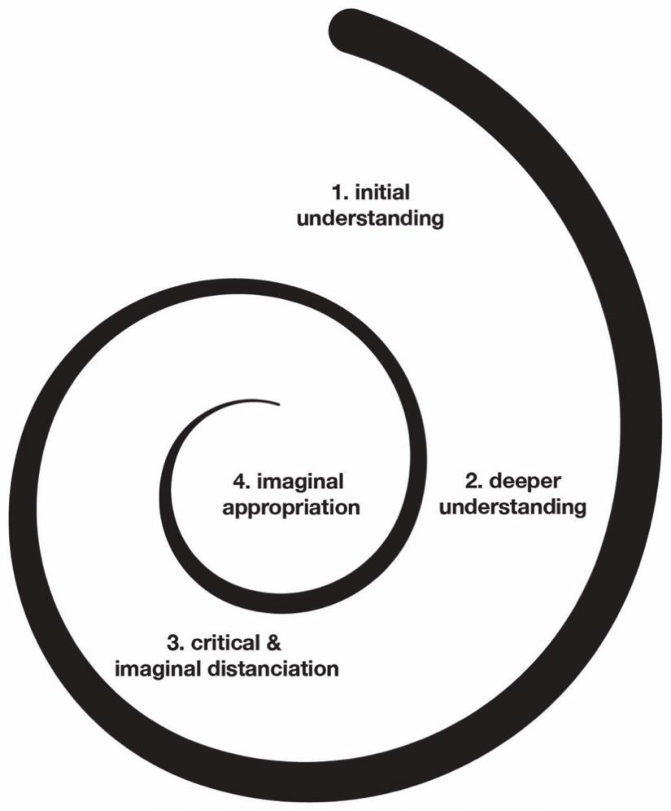
\includegraphics[scale=0.5]{fig/HS.png}
    \caption{Hermenutic Spiral \cite{hermeneutics}}
\end{figure}

%\section{Research Areas}

%The different configurations we presented as options to the client gives us ample opportunity to answer several questions raised by the limitations of the current design. We will investigate closer how the current design works, and then contrast that with our designs. This will allow us to compare speed in regards to frame per second on image processing, the advantages and disadvantages of a distributed approach contrasted with the central approach that exists today and possible limitations and disadvantages on a distributed approach, as it is likely we will not be able to say with absolute certainty that one approach fits all in every scenario.\\

%\section{intro 2.0?}

%Cameras are commonly used as sensors for autonomous vehicles due to their versatility, low cost and untapped potential. A downside is that doing something meaningful with camera images can be very computationally expensive. Let’s say we want to process a 24-bit color image with a 600x600 resolution pixel-by-pixel. That’s 360 000 pixels with 3 color channels each, giving us an input data size of 1 080 000 bytes per image. A common task for an autonomous vehicle is real-time object detection, which requires the system to run the image input through complex algorithms multiple times per second.

%The hardware required to perform real-time object detection is widely available today in the form of consumer-grade CPUs and GPUs. However, a problem arises if the autonomous vehicle has any restrictions on weight, physical space and power consumption, which is the case with small Unmanned Aerial Vehicles (UAV).

%In previous years, the participants of KDA’s Local Hawk summer project have attempted to run object detection on a lightweight UAV. Their attempts have not led anywhere as the detection framerate at around 1 frame per second was too low for any meaningful functionality. Their results were achieved by using a single Raspberry Pi 4 for all the UAV’s computations.

%This study aims to explore multiple software and hardware architectures for a small UAV with object detection capabilities. The configurations will be compared in terms of performance, cost, complexity and weight. Our results will provide recommendations on which technology to use when building lightweight UAVs for various use cases which require object detection.\\



%\subsection{Customer}

%The customer for this project was Kongsberg Gruppen, a local technology company with a global presence in the fields of defense, aerospace, maritime, and digital industries. \\

%The results of this project will be used in KDAs summer internship project “Local Hawk”, where they develop autonomous UAV (Unmanned Aerial Vehicles) over the summer. \\

%Throughout the duration of the project, Kongsberg Gruppen provided valuable insights, feedback, and guidance, which helped shape the project's direction and ensured its success. Regular meetings and communication with the customer allowed the team to stay aligned with their expectations and make any necessary adjustments to the project's scope and objectives. \\






\newpage



\chapter{Process}
\label{ch:process}
\title{Process}

In this section, we will outline and explain how we transitioned from our initial phase and organized our project in order to facilitate work on practical implementation. We will explain which tools we utilized and the methodology we used to achieve our results.  \\

While the hermeneutic methodology facilitated invaluable insights during the exploratory stage of our project, its emphasis on interpretation and understanding proved less applicable when transitioning from knowledge acquisition to knowledge application. The hermeneutic approach, with its focus on understanding texts or phenomena in depth, provides a foundation for comprehensive understanding rather than prioritizing explicit task completion. Consequently, as the project shifted to a phase demanding direct action and the tangible execution of tasks, the inherent characteristics of the hermeneutic approach were less aligned with these new requirements. Therefore, to maintain project efficiency during the implementation phase, it became necessary to consider alternative methodologies more attuned to the objectives of this new stage.\\

We decided that our project demands were best met using an agile methodology. This methodology is an iterative approach to software development and project management that emphasizes flexibility, collaboration, and client satisfaction. It advocates adaptive planning, evolutionary development, early delivery, continual improvement, and encouraging rapid and flexible response to change. Agile methods break tasks into smaller increments with minimal planning and do not directly involve long-term planning. This methodology prioritizes direct communication over extensive documentation, producing working software that evolves through a collaborative effort between self-organizing cross-functional teams. \\

\begin{figure}[H]
    \centering
    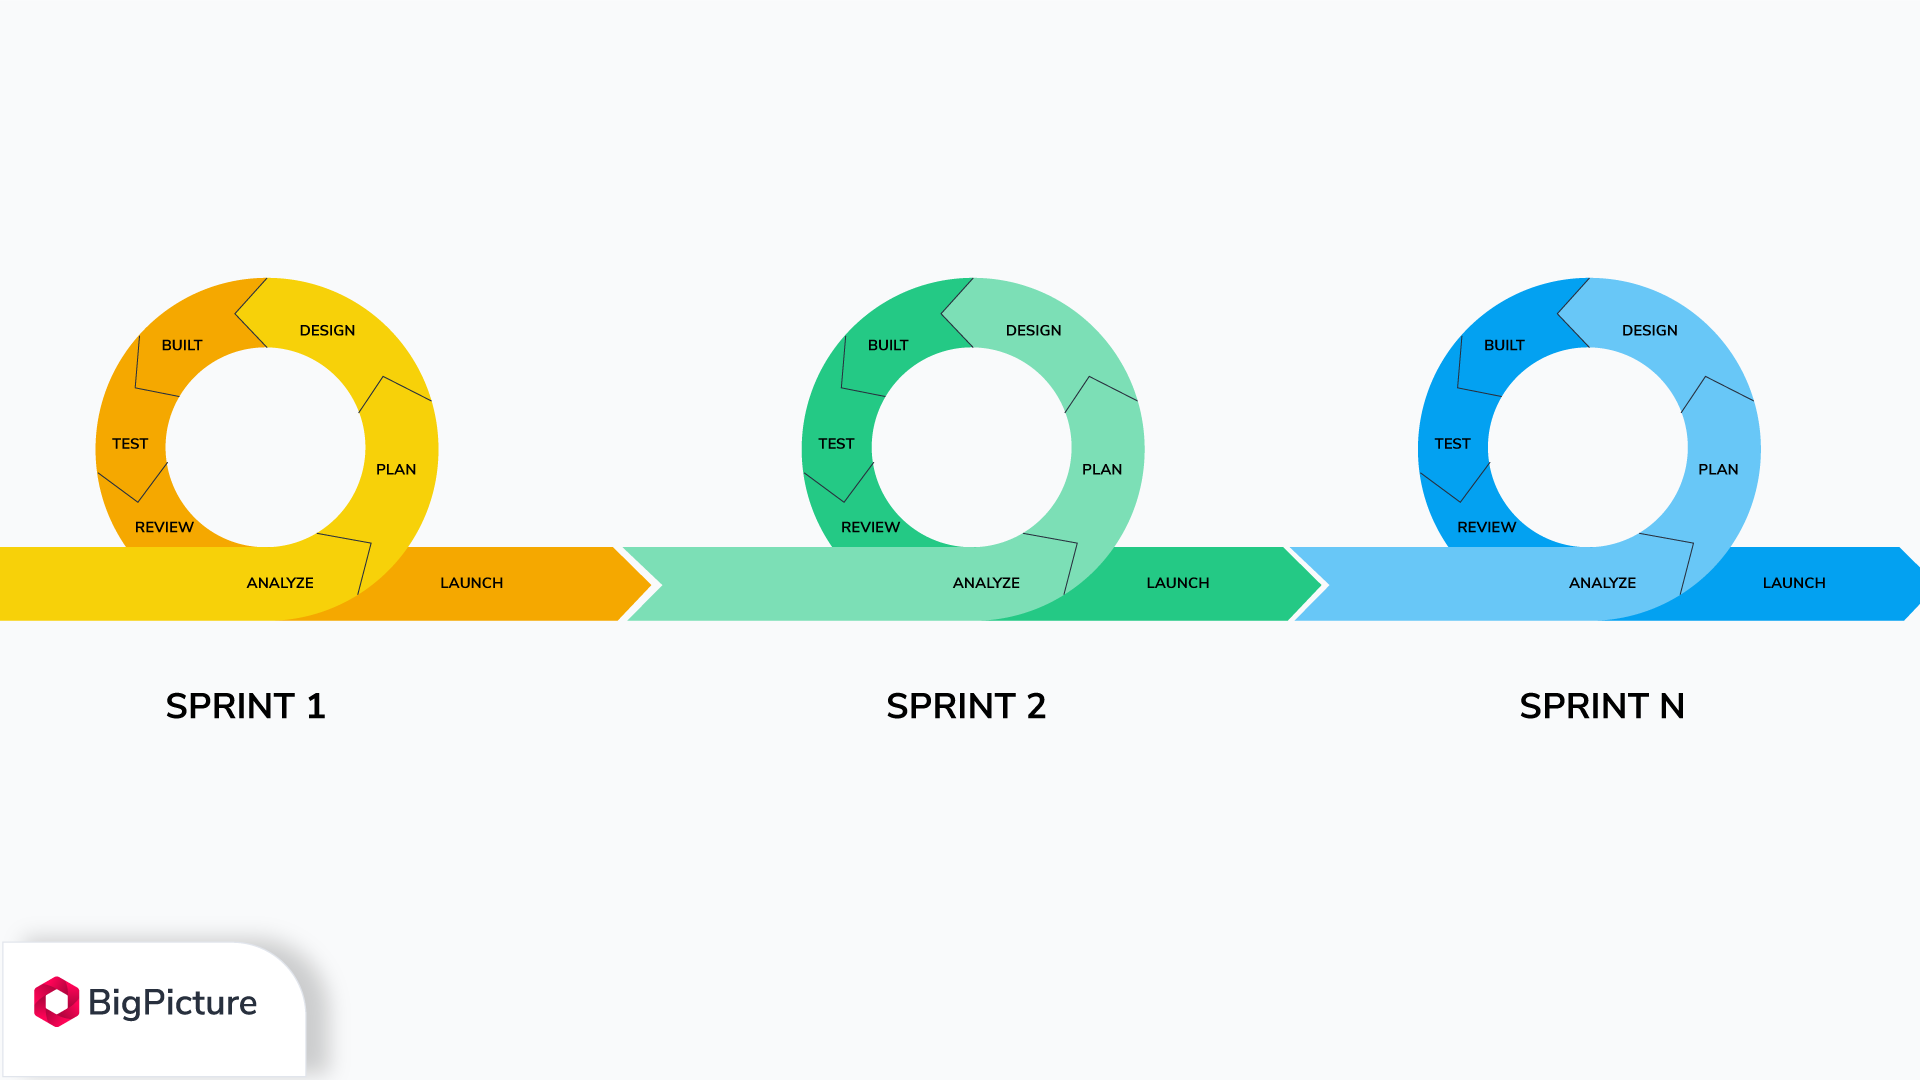
\includegraphics[scale=0.25]{fig/sprints.png}
    \caption{Sprint organization \cite{sprintimage}}
\end{figure}

An agile workflow has a number of key terms and features, and there are several different ways to conduct an agile project. Common for all of these, however, is that these projects are divided into short work cycles known as iterations or sprints, typically lasting between one and four weeks. Each sprint has a defined goal and a set of tasks to be completed. We decided that for our project we would not adhere to a strict definition, e.g., scrum. Instead, we opted to pick and choose between different features that made the most sense for our project, and to make sure that we utilized the most prominent features that are essential to an agile project. These features were: sprint, sprint backlog, daily stand-up meetings, and retrospective.\\

Following the agile methodology, we decided to have daily stand-up meetings where we would update the group on our individual progress. We organized our sprints to last one week at a time, where we had an initial meeting on Monday to set up our tasks for the week, and a meeting at the end of the week where we updated our client on where we were in terms of progress. In the end-of-week meetings, the client was invited to give feedback on which tasks they wanted us to prioritize going forward into the next sprint.\\

\section{Project Tools}

\subsection{Github}

We needed a way to organize and collaborate on code, and essential to this is Source Code Management (SCM), and for this purpose, our choice fell on git. Git is a distributed SCM, originally developed for use on the Linux kernel, but has since gained a significant market share and is now the dominant SCM. Git's primary function is to enable developers to create different versions of their projects and switch between these versions seamlessly. This means that developers can experiment with different features and code changes without impacting the main, stable codebase. If a change works well, it can be integrated (or "merged") into the main codebase; if not, it can be discarded without having caused any disruption.\\

In a team environment, Git is essential for managing contributions from multiple developers. Each developer can work on their own copy of the project (a "branch"), without interfering with others' work. When their work is complete, it can be merged into the main codebase.\\

Git is also distributed, meaning every developer has a complete copy of the project's history on their local machine. This not only allows developers to work offline but also provides an inherent backup. If any repository is lost, it can be restored from any developer's local copy.\\

Instead of organizing our own server with git, we opted for using GitHub, which allows students and educators access to their professional option at no cost, allowing us to organize our code in a more structured manner. \\

\subsection{Taiga}
In order to organize our agile workflow we elected to use Taiga. It is a web-based tool that allows us to track sprints, tasks within sprints, and assign aforementioned tasks to specific members of the group, and additionally allow members to follow updates on a specific task. In addition to this, Taiga has integration with GitHub, allowing us to modify tasks from GitHub whenever we commit code in our repository there.


\begin{figure}[h]
    \centering
    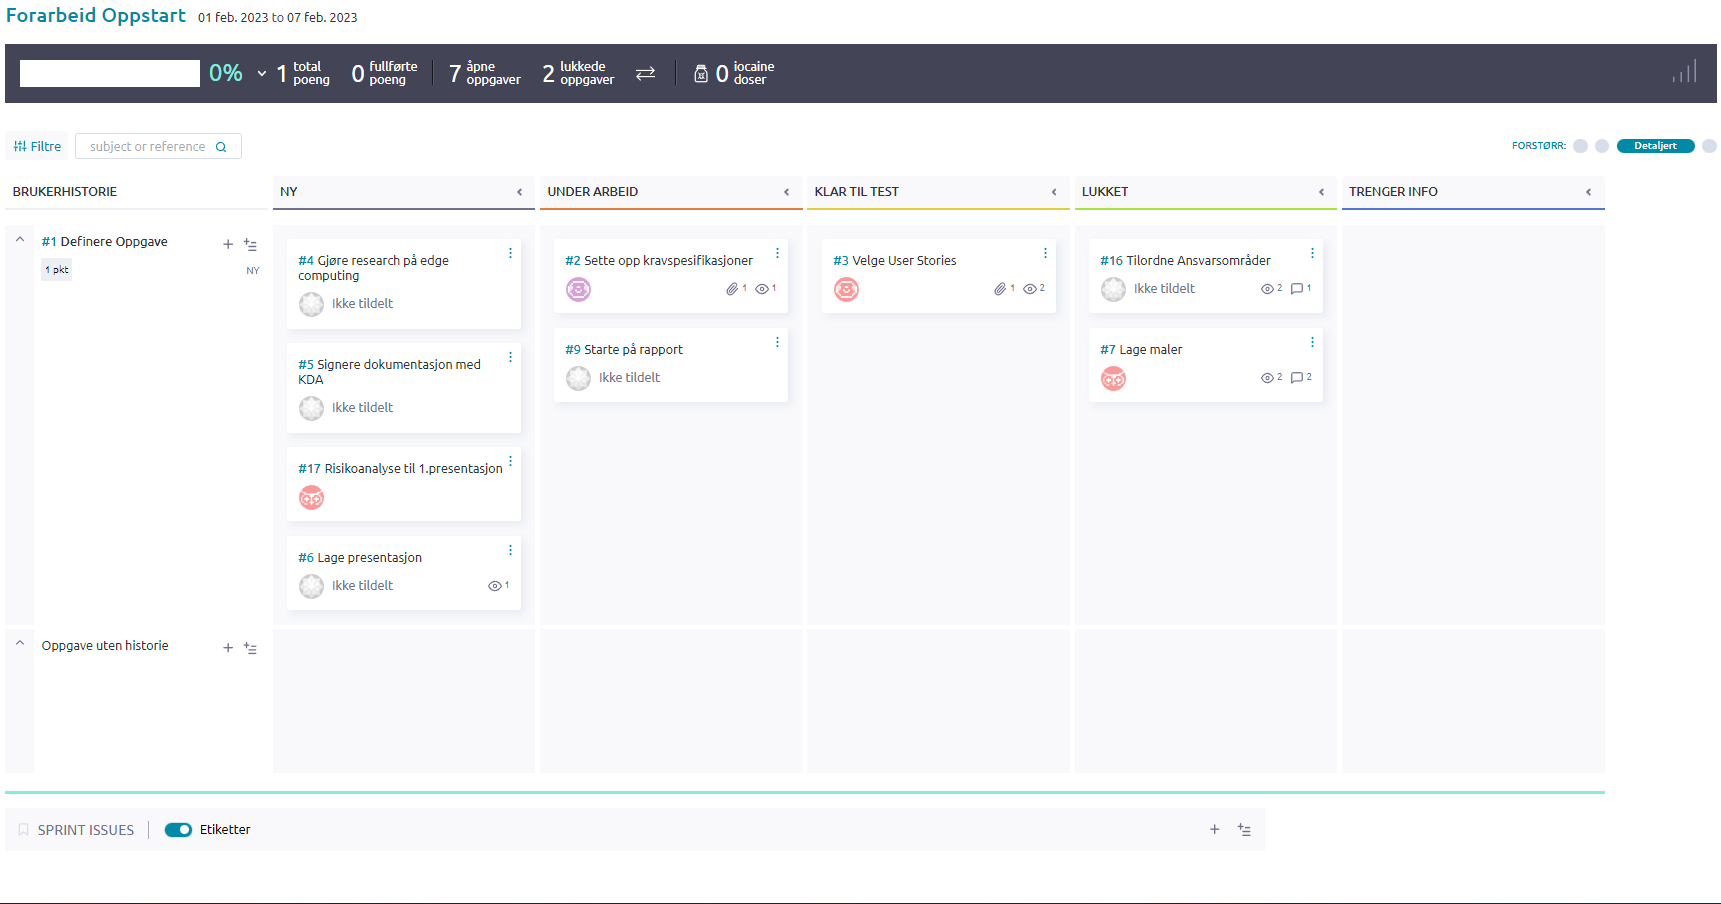
\includegraphics[width=\textwidth]{fig/Taiga eksempel.png}
    \caption{Taiga Interface}
\end{figure}

As the project progressed, we found that we were not generating a substantial amount of code, and therefore, the GitHub integration was not as crucial as we initially assumed. Moreover, our interaction with the Taiga platform was proving to be more of a diversion from our core tasks rather than a facilitator of our work. The platform's organization and functionality did not meet our needs and expectations, which caused further dissatisfaction. Consequently, we decided to transition away from this web-based project management tool. Instead, we opted for a more streamlined approach of crafting summaries for each sprint. This method proved to be less demanding in terms of resources and was more suitable and beneficial for the progression of our project.\\


\subsection{Overleaf}
Overleaf is a collaborative, cloud-based LaTeX editor used for the creation of scientific documents. LaTeX is a typesetting system favored in academia for its ability to handle technical and scientific documents with ease, especially those with complex mathematical equations or structures.\\

Overleaf provides a platform where multiple users can view, edit, and compile LaTeX documents in real time. This collaboration aspect makes it an excellent tool for group projects, theses, papers, or any document requiring input from several contributors.\\

\subsection{ChatGPT}
ChatGPT is an artificial intelligence language model, released to the public recently. It is designed to understand natural language and generate human-like responses to a wide range of prompts and questions.\\

ChatGPT is most useful for tasks that require natural language processing, such as language translation, sentiment analysis, text summarization, and conversational interfaces. It can also be used for a variety of other applications, such as content generation, language modeling, and knowledge extraction.\\

We have on occasion used ChatGPT for cleaning up and helping us formulate language in a more academic and formal fashion.\\

\subsection{Microsoft Suite}
Microsoft Office is a suite of productivity applications that have become a standard tool in most professional and academic environments. It includes software like Word for document creation, Excel for data management and analysis, PowerPoint for presentations, Outlook for email and calendar management, and more recently Teams for collaborative communication. Each of these applications serves distinct purposes and can be instrumental in managing and executing a project efficiently.\\

For our purposes, we organized a lot of our work through the university-provided teams solution, where we organized documents that were impractical to use LaTeX for. This is where we kept time sheets, presentation material, and meeting notes. \\

\newpage
\section{Risk Analysis}

Risk analysis is an ongoing process that continuously evaluates risk throughout the project's lifecycle. It is the responsibility of the risk manager to ensure that this process takes place regularly and consistently during the project. This is crucial because it raises awareness among us and our client about potential risks and vulnerabilities, encourages necessary improvements, and facilitates necessary changes. Such analysis can help the risk manager to identify new risks and changes that require attention along the way. \cite{Risk1}

After identifying the risks, it is essential to prioritize them based on their probability and consequence. Moreover, measures should be put in place to manage them effectively if they occur. While everyone on the team should participate in assessing the project's risks, the risk manager will be primarily responsible for ensuring quality assurance. \cite{Risk2}

\subsubsection{Identifying the risks in our project}
A risk analysis was conducted for our project, wherein we identified both internal and external risks. Internal risks are linked with factors that are under our control, whereas external risks are associated with factors that lie beyond our control.\cite{RiskInternalExternal}

After identifying the risks at this stage, we evaluate their potential consequences and determine the appropriate measures that can be taken if they occur. To gain a better overview, we record the risks in a table that includes a unique code, a description of the risk event, recommended measures, probability (P), consequence (C), and priority. Below is a comprehensive overview of both internal and external risks:


\begin{figure}
\centering
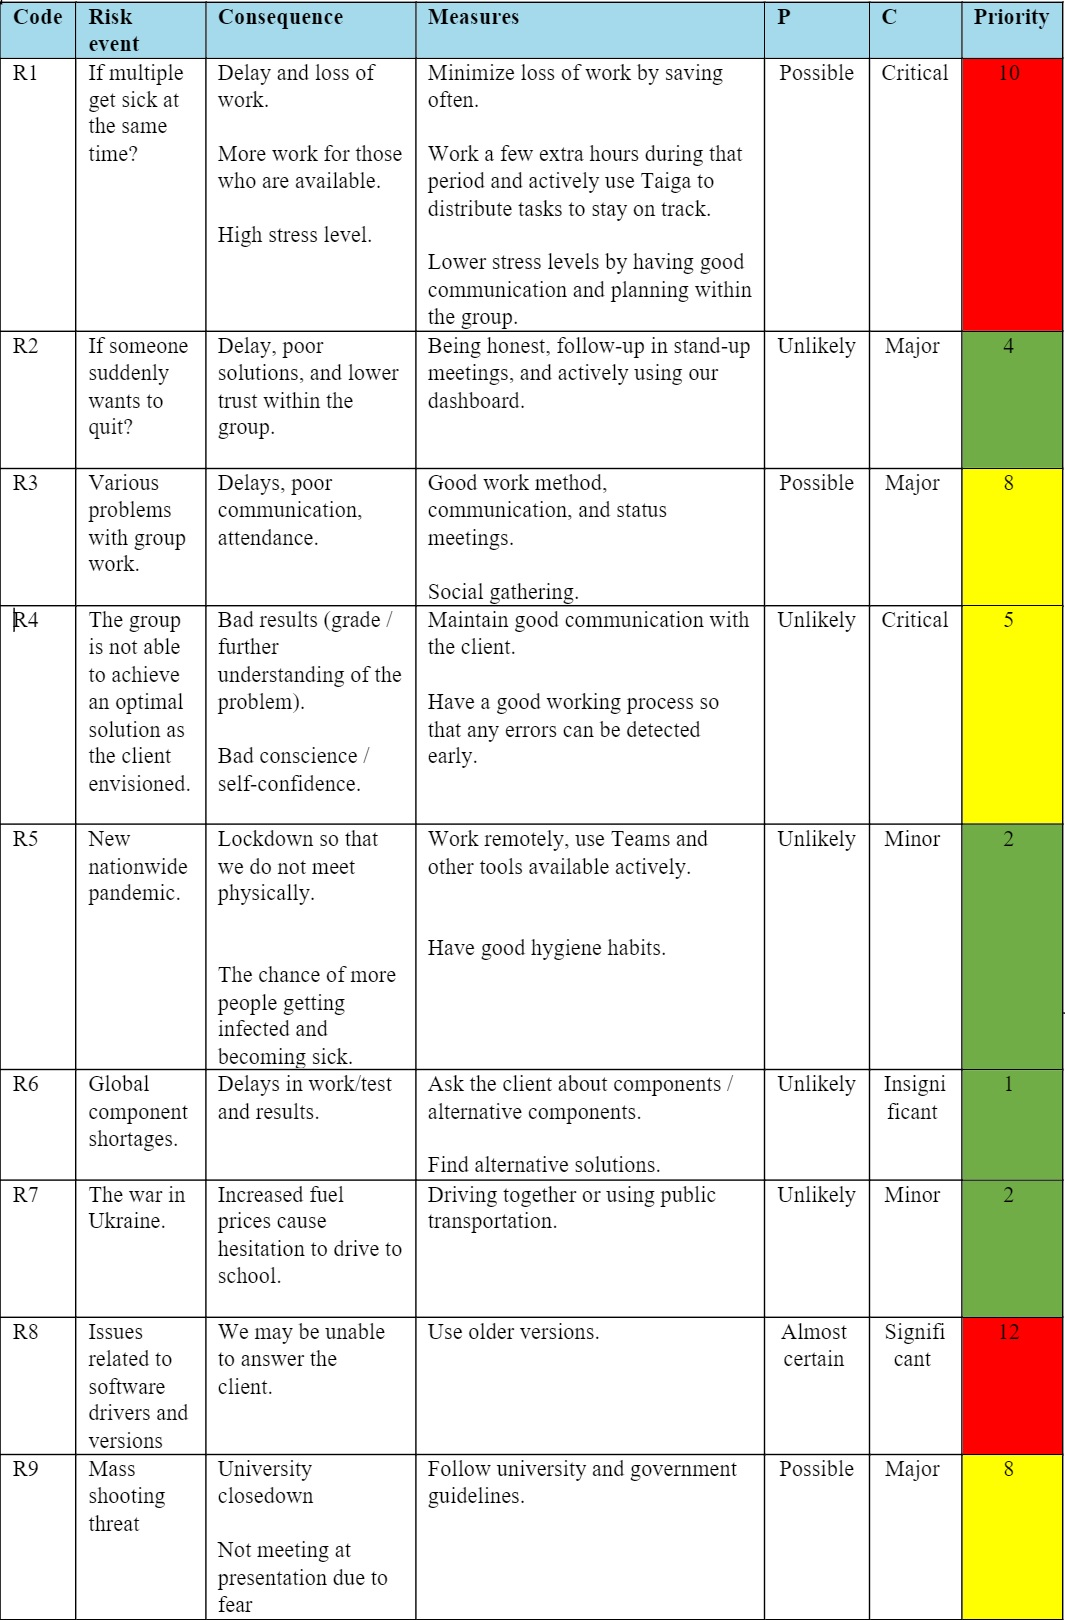
\includegraphics[width=0.80\linewidth]{fig/RisikoTabell.jpg}
\caption{Risk table}
\label{fig:Risktable}
\end{figure}

\newpage

The prioritization of these risks was determined by evaluating their consequence and probability using the risk matrix:

\begin{figure}[h!]
\centering
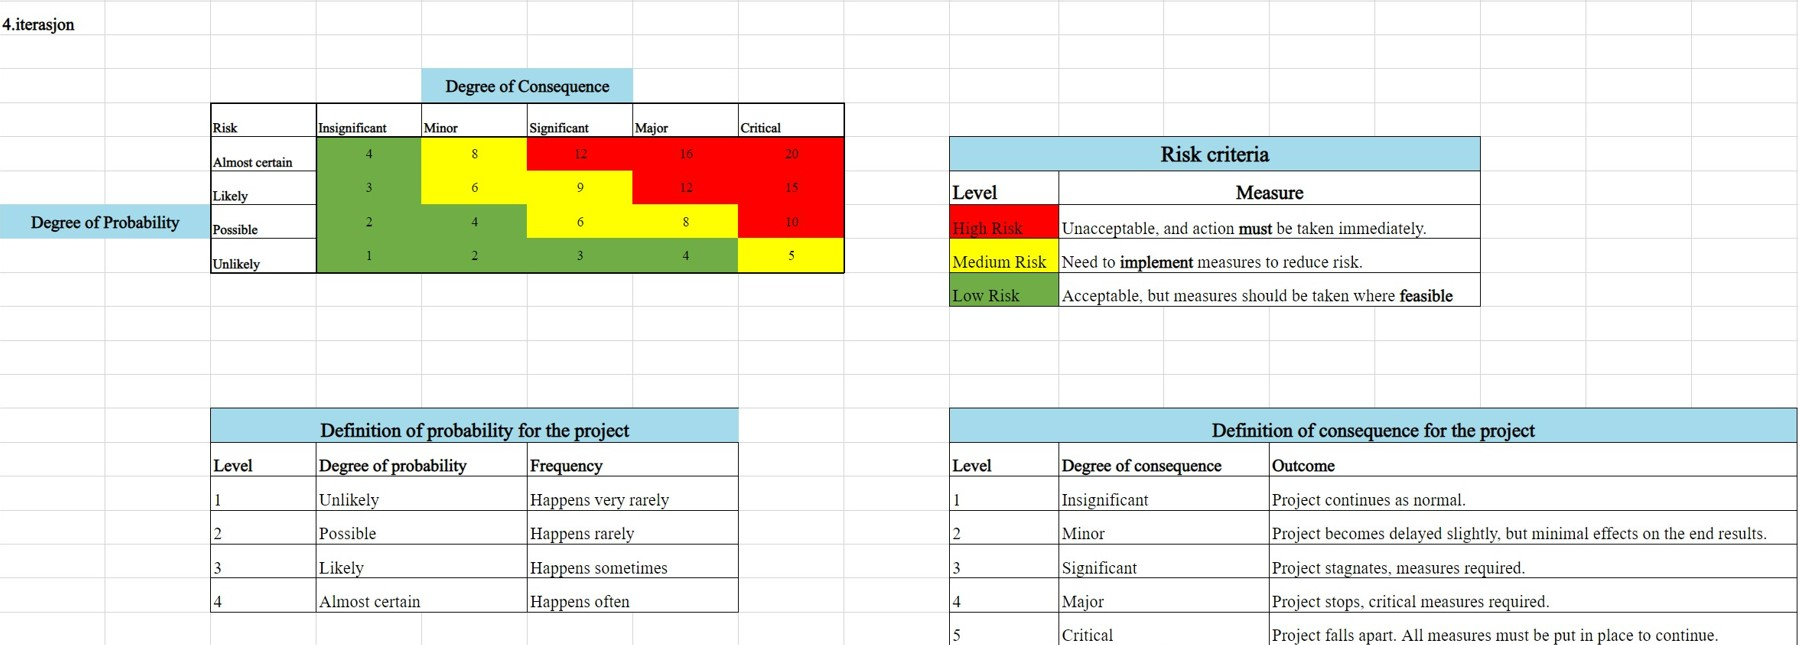
\includegraphics[width=0.85\linewidth]{fig/RiskMatrix.jpg}
\caption{Risk Matrix \cite{RiskMatrix}} 
\label{fig:RiskMatrix}
\end{figure}
\newpage

%\chapter{Project Tools}
%\label{ch:projecttools}
%\input{Kapitler/Project Tools}

%\chapter{Hardware}
%\label{ch:hardware}
%\iffalse
A single-board computer Ż.Ŵ Image processing configurations
TODO: TABELL MED OVERSIKT OVER CONFIGS
Table 8.1: Image processing configurations
Hardware Computer Vision
Software
Weight
Config 1 Nvidia Jetson
Nano, ArduCamŻ.Ŵ Image processing configurations
TODO: TABELL MED OVERSIKT OVER CONFIGS
Table 8.1: Image processing configurations
Hardware Computer Vision
Software
Weight
Config 1 Nvidia Jetson
Nano, ArduCam
Mini
TensorRT,
YOLOv5
...
Config 2 Raspberry Pi 4,
Coral Edge TPU,
Pi Camera 3.0
OpenCV, Tensor-
Flow Lite
...
Config 3 Raspberry Pi Zero
Mini
TensorRT,
YOLOv8
...
Config 2 Raspberry Pi 4,
Coral Edge TPU,
Pi Camera 3.0
OpenCV, Tensor-
Flow Lite
...
Config 3 Raspberry Pi Zero 
\fi

\title{Hardware}
\section{Specification tables for configs}

All values from these tables that are not referenced externally are done by own measuring.\\
The power supply component for the single-board computers has been omitted from these tables due to there being several different options to choose from when supplying power to these boards and not all of them can be covered here.

\subsection{Config 1}

\begin{table}[!htb]
\begin{tabular}{ | >{\raggedright}p{\dimexpr 0.30\linewidth-2\tabcolsep} |
                   >{\raggedleft}p{\dimexpr 0.14\linewidth-2\tabcolsep} |
                   >{\raggedleft}p{\dimexpr 0.14\linewidth-2\tabcolsep} |
                   >{\raggedleft}p{\dimexpr 0.14\linewidth-2\tabcolsep} |
                    >{\raggedleft}p{\dimexpr 0.14\linewidth-2\tabcolsep} |
                   >{\raggedleft\arraybackslash}p{\dimexpr 0.14\linewidth-2\tabcolsep} | } \hline

&\bfseries{MSRP} & \bfseries{Weight} & \bfseries{Volume} & \bfseries{Power} (idle)   & \bfseries{Power (max)}    \\\hline

\bfseries{Jetson Nano}      & \$ 99     & 241 g     & 232 cm$^{3}$  & 5 W       & 10 W      \\\hline
\bfseries{Pi camera 3}      & \$ 25     & 4 g       & 7 cm$^{3}$    & 0,66 W    & 0,83 W    \\\hline
\bfseries{Camera ribbon}    & -         & 1,1 g     & -             & -         & -         \\\hline
\bfseries{SUM}              & \$ 124    & \bfseries{246,1 g}   & \bfseries{239 cm$^{3}$}    & \bfseries{5,7 W}    & \bfseries{10,8 W}    \\\hline
\end{tabular}
\caption{Hardware specification table for Config 1 hardware \cite{Jetson}\cite{specifications-cameras}}
\label{tab:spec_table_Config1}
\end{table}


\subsection{Config 2}

\begin{table}[!htb]
\begin{tabular}{ | >{\raggedright}p{\dimexpr 0.30\linewidth-2\tabcolsep} |
                   >{\raggedleft}p{\dimexpr 0.14\linewidth-2\tabcolsep} |
                   >{\raggedleft}p{\dimexpr 0.14\linewidth-2\tabcolsep} |
                   >{\raggedleft}p{\dimexpr 0.14\linewidth-2\tabcolsep} |
                    >{\raggedleft}p{\dimexpr 0.14\linewidth-2\tabcolsep} |
                   >{\raggedleft\arraybackslash}p{\dimexpr 0.14\linewidth-2\tabcolsep} | } \hline

&\bfseries{MSRP} & \bfseries{Weight} & \bfseries{Volume} & \bfseries{Power} (idle)   & \bfseries{Power (max)}    \\\hline

\bfseries{Raspberry Pi 4B 4GB}  & \$ 60     & 46 g      & 86 cm$^{3}$   & 2,7 W     & 6,4 W     \\\hline
\bfseries{Pi camera 3}          & \$ 25     & 4 g       & 7 cm$^{3}$    & 0,66 W    & 0,83 W    \\\hline
\bfseries{Camera ribbon}        & -         & 1,1 g     & -             & -         & -         \\\hline
\bfseries{Coral USB}            & \$ 60     & 19,7 g    & 15,6 cm$^{3}$ & 2,5 W     & 4,5 W     \\\hline
\bfseries{USB C-A cable}        & -         & 16,8 g    & -             & -         & -         \\\hline
\bfseries{SUM}                  & \$ 145 & \bfseries{87,6 g}   & \bfseries{109 cm$^{3}$}    & \bfseries{5,7 W}    & \bfseries{11,7 W}    \\\hline
\end{tabular}
\caption{Hardware specification table for Config 2 hardware \cite{datasheet-RPi4B}\cite{power-consumption-RPi4}\cite{specifications-cameras}\cite{CoralTPU}}
\label{tab:spec_table_Config2}
\end{table}

\newpage

\subsection{Config 3}

\begin{table}[!htb]
\begin{tabular}{ | >{\raggedright}p{\dimexpr 0.30\linewidth-2\tabcolsep} |
                   >{\raggedleft}p{\dimexpr 0.14\linewidth-2\tabcolsep} |
                   >{\raggedleft}p{\dimexpr 0.14\linewidth-2\tabcolsep} |
                   >{\raggedleft}p{\dimexpr 0.14\linewidth-2\tabcolsep} |
                    >{\raggedleft}p{\dimexpr 0.14\linewidth-2\tabcolsep} |
                   >{\raggedleft\arraybackslash}p{\dimexpr 0.14\linewidth-2\tabcolsep} | } \hline

&\bfseries{MSRP} & \bfseries{Weight} & \bfseries{Volume} & \bfseries{Power} (idle)   & \bfseries{Power (max)}    \\\hline

\bfseries{Raspberry Pi Zero2}   & \$ 15     & 11 g      & 9,75 cm$^{3}$     & 0,6 W     & 6,4 W     \\\hline
\bfseries{Pi camera 3}          & \$ 25     & 4 g       & 7 cm$^{3}$        & 0,66 W    & 0,83 W    \\\hline
\bfseries{Camera ribbon}        & -         & 1,1 g     & -                 & -         & -         \\\hline
\bfseries{Coral USB}            & \$ 60     & 19,7 g    & 15,6 cm$^{3}$     & 2,5 W     & 4,5 W     \\\hline
\bfseries{USB C-micro cable}    & -         & 7,5 g     & -                 & -         & -         \\\hline
\bfseries{SUM}                  & \$ 100 & \bfseries{43,3 g}   & \bfseries{32 cm$^{3}$}    & \bfseries{3,8 W}    & \bfseries{11,7 W}    \\\hline
\end{tabular}
\caption{Hardware specification table for Config 3 hardware \cite{datasheet-RPiZero2}\cite{power-consumption-RPiZero2}\cite{specifications-cameras}\cite{CoralTPU}}
\label{tab:spec_table_Config3}
\end{table}



\subsection{Config 4}

\begin{table}[!htb]
\begin{tabular}{ | >{\raggedright}p{\dimexpr 0.30\linewidth-2\tabcolsep} |
                   >{\raggedleft}p{\dimexpr 0.14\linewidth-2\tabcolsep} |
                   >{\raggedleft}p{\dimexpr 0.14\linewidth-2\tabcolsep} |
                   >{\raggedleft}p{\dimexpr 0.14\linewidth-2\tabcolsep} |
                    >{\raggedleft}p{\dimexpr 0.14\linewidth-2\tabcolsep} |
                   >{\raggedleft\arraybackslash}p{\dimexpr 0.14\linewidth-2\tabcolsep} | } \hline

&\bfseries{MSRP} & \bfseries{Weight} & \bfseries{Volume} & \bfseries{Power} (idle)   & \bfseries{Power (max)}    \\\hline

\bfseries{Raspberry Pi 4B}  & \$ 60     & 46 g      & 86 cm$^{3}$   & 2,7 W     & 6,4 W     \\\hline
\bfseries{Pi camera 3}      & \$ 25     & 4 g       & 7 cm$^{3}$    & 0,66 W    & 0,83 W    \\\hline
\bfseries{Camera ribbon}    & -         & 1,1 g     & -             & -         & -         \\\hline
\bfseries{SUM}              & \$ 85 & \bfseries{51,1 g} & \bfseries{93 cm$^{3}$}  & \bfseries{3,4 W}  & \bfseries{7,2 W}    \\\hline

\end{tabular}
\caption{Hardware specification table for Config 4 hardware \cite{datasheet-RPi4B}\cite{power-consumption-RPi4}\cite{specifications-cameras}}
\label{tab:spec_table_Config4}
\end{table}

\subsection{Comparison}

\begin{table}[!htb]
\begin{tabular}{ | >{\raggedright}p{\dimexpr 0.30\linewidth-2\tabcolsep} |
                   >{\raggedleft}p{\dimexpr 0.14\linewidth-2\tabcolsep} |
                   >{\raggedleft}p{\dimexpr 0.14\linewidth-2\tabcolsep} |
                   >{\raggedleft}p{\dimexpr 0.14\linewidth-2\tabcolsep} |
                    >{\raggedleft}p{\dimexpr 0.14\linewidth-2\tabcolsep} |
                   >{\raggedleft\arraybackslash}p{\dimexpr 0.14\linewidth-2\tabcolsep} | } \hline

&\bfseries{MSRP} & \bfseries{Weight} & \bfseries{Volume} & \bfseries{Power} (idle)   & \bfseries{Power (max)}    \\\hline

\bfseries{Config 1}& \$ 124     & 246,1 g   & 239 cm$^{3}$  & 5,7 W     & 10,8 W    \\\hline
\bfseries{Config 2}& \$ 145     & 87,6 g    & 109 cm$^{3}$  & 5,7 W     & 11,7 W    \\\hline
\bfseries{Config 3}& \$ 100    & 43,3 g    & 32 cm$^{3}$   & 3,8 W     & 11,7 W    \\\hline
\bfseries{Config 4}& \$ 85    & 51,1 g    & 93 cm$^{3}$   & 3,4 W     & 7,2 W     \\\hline

\end{tabular}
\caption{Hardware specification table for comparison of all configs}
\label{tab:spec_table_comparison}
\end{table}

\section{Single-board computer (SBC)}

A single-board computer (SBC) is a complete computer built on a single circuit board, with microprocessor(s), memory, input/output (I/O) and other features required of a functional computer. Single-board computers are commonly made as demonstration or development systems, for educational systems, or for use as embedded computer controllers. Many types of home computers or portable computers integrate all their functions onto a single printed circuit board.

Unlike a desktop personal computer, single board computers often do not rely on expansion slots for peripheral functions or expansion. Single board computers have been built using a wide range of microprocessors. Simple designs, such as those built by computer hobbyists, often use static RAM and low-cost 32- or 64-bit processors like ARM. Other types, such as blade servers, would perform similar to a server computer, only in a more compact format. \cite{SBC}

Thanks to the characteristics of SBCs, they are a core hardware component in all of the architectural designs in this comparative study.

\newpage
\begin{table}
\begin{tabular}{ | >{\raggedright}p{\dimexpr 0.19\linewidth-2\tabcolsep} |
                   >{\raggedleft}p{\dimexpr 0.27\linewidth-2\tabcolsep} |
                   >{\raggedleft}p{\dimexpr 0.27\linewidth-2\tabcolsep} |
                   >{\raggedleft\arraybackslash}p{\dimexpr 0.27\linewidth-2\tabcolsep} | } \hline

                            & \centering\bfseries{RPi 4B} & \centering\bfseries{RPi Zero2} & \centering\arraybackslash\bfseries{Jetson Nano}\\\hline
\bfseries{CPU}              & Cortex-A72 @ 1.5GHz       & Cortex-A53 @ 1.0GHz   & Cortex-A57 @ 1.43GHz \\\hline
\bfseries{GPU}              & VideoCore IV @ 500MHz     & VideoCore IV @ 400MHz & 128-core Maxwell @ 921MHz \\\hline
\bfseries{Memory}           & 1 GB - 8 GB               & 512 MB                & 4 GB \\\hline
\bfseries{Video decoding}   & H.264/H.265 (4Kp60)       & H.264 (1080p30)       & H.264/H.265 (4Kp60) \\\hline
\bfseries{Video encoding}   & H.264/H.265 (1080p30)     & H.264 (1080p30)       & H.264/H.265 (4Kp30) \\\hline
\bfseries{Connectivity}     & USB 3.0 × 2               & USB 2.0 × 1           & USB 3.0 × 4 \\
                            & USB 2.0 × 2               & UART × 1              & USB 2.0 × 1 \\
                            & UART × 1                  & SPI × 2               & UART × 1 \\
                            & SPI × 2                   & I2C × 1               & SPI × 2 \\
                            & I2C × 1                   &                       & I2C × 3 \\\hline
\bfseries{Form factor}      & 85mm × 56mm               & 65mm × 30mm           & 69mm × 45mm \\\hline
\bfseries{Weight}           & 46g                       & 11g                   & 250g \\\hline
\bfseries{MSRP}             & \$ 35 - \$ 75             & \$ 15                 & \$ 99 \\\hline

\end{tabular}
\caption{Comparison table for single-board computers (SBCs) \protect\cite{datasheet-RPiZero2}\cite{datasheet-RPi4B}\cite{datasheet-JetsonNano}}
\label{tab:comparison_table_SBCs}
\end{table}

When proposing what SBCs to deploy in our test-solution architectures we tend to mainly look at specifications regarding processing power (CPU \& GPU), memory (RAM), hardware-accelerated video encoding/decoding and connectivity (USB, UART etc.) in relation to the weight and form factor of the board. We also need to take into consideration the availability and discrepancy between MSRP and actual sale price due to the current world-wide chip shortage disrupting the market.\\

We decided the top-contenders and implemented them across all configurations:
\begin{itemize}
    \item Raspberry Pi Zero 2 (RPi Zero 2)
    \item Raspberry Pi 4B (RPi 4B)
    \item nVidia Jetson Nano
\end{itemize}

% Fjerne denne? Usikker:
\iffalse
\subsection{nVidia Jetson Nano}
Jetson Nano Developer Kit is a compact, high-performance computer designed to run multiple neural networks simultaneously for applications such as image classification, object detection, segmentation, and speech processing. It enables developers to build AI-powered applications and projects using GPU acceleration. The Jetson Nano comes with a quad-core ARM CPU, NVIDIA GPU with 128 CUDA cores, and 4GB of RAM, making it suitable for applications like robotics, computer vision, and edge computing.\cite{Jetson}

\begin{figure}[h]
    \centering
    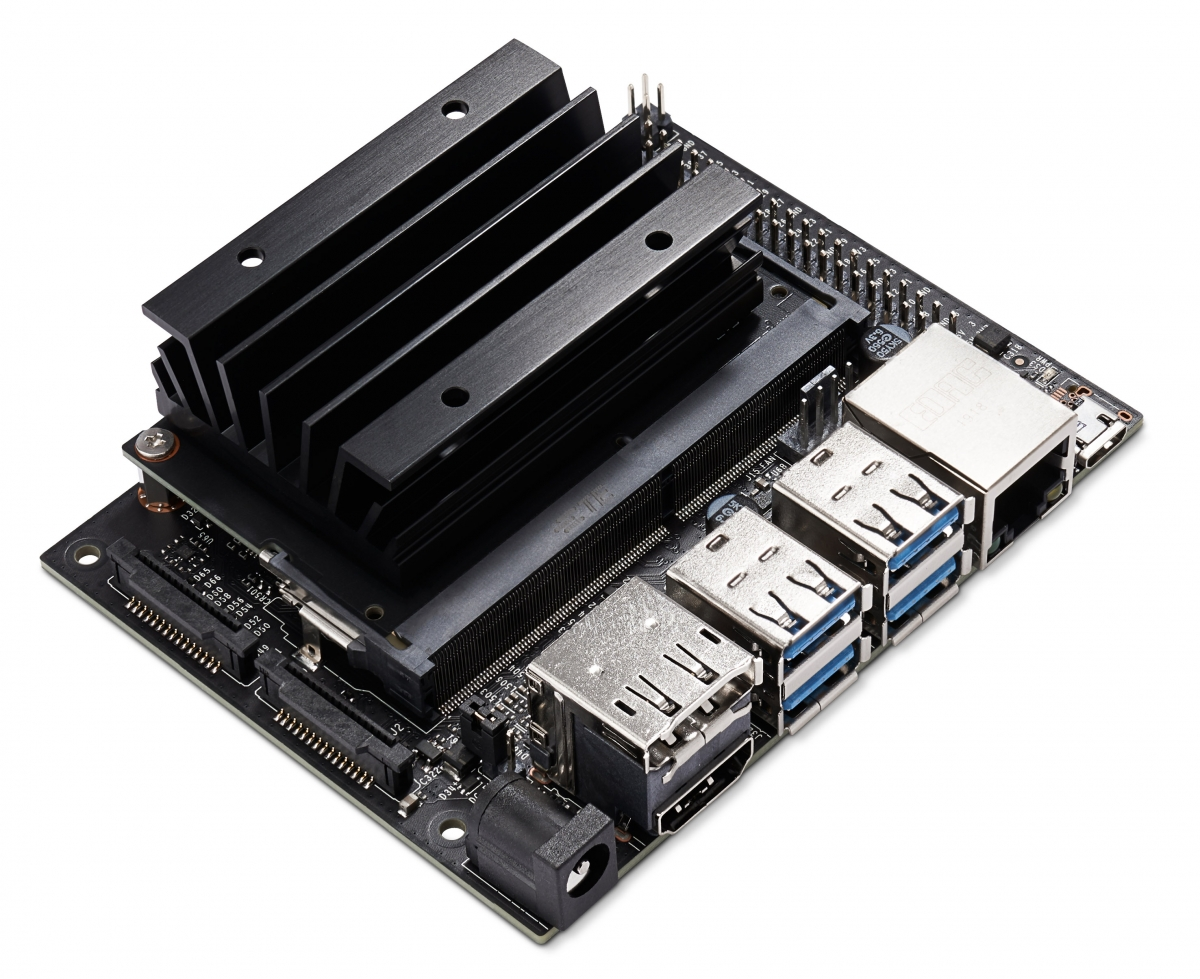
\includegraphics[scale=0.3]{fig/JetsonNano-DevKit_Front-Top_Right_trimmed.jpg}
    \caption{Jetson nano \cite{Jetson}}
\end{figure}
\fi


\newpage

\section{Camera}

\begin{table}[!h]
\begin{tabular}{ | >{\raggedright}p{\dimexpr 0.25\linewidth-2\tabcolsep} |
                   >{\raggedleft}p{\dimexpr 0.25\linewidth-2\tabcolsep} |
                   >{\raggedleft}p{\dimexpr 0.25\linewidth-2\tabcolsep} | 
                   >{\raggedleft\arraybackslash}p{\dimexpr 0.25\linewidth-2\tabcolsep} | } \hline

& \centering\bfseries{Camera Module v2}   & \centering\bfseries{Camera Module 3 NoIR}   & \centering\arraybackslash\bfseries{Camera Module 3 Wide} \\\hline
\bfseries{Video Modes}
& 1920 × 1080p47                & 2304 × 1296p56                    & 2304 × 1296p56 \\
& 1640 × 1232p41                & 2304 × 1296p30                    & 2304 × 1296p30 \\
& 640 × 480p206                 & 1536 × 864p120                    & 1536 × 864p120 \\\hline
\bfseries{Focus}
& Adjustable                    & Motorized                         & Motorized  \\\hline
\bfseries{Depth of field}
& Approx 10 cm to ∞             & Approx 10 cm to ∞                 & Approx 5 cm to ∞ \\\hline
\bfseries{Horizontal FoV}
& 62.2 degrees                  & 66 degrees                        & 102 degrees \\\hline
\bfseries{Vertical FoV}
& 48.8 degrees                  & 41 degrees                        & 67 degrees \\\hline
\bfseries{Size}
& 25 × 24 × 9mm                 & 25 × 24 × 11.5mm                  & 25 × 24 × 12.4mm \\\hline
\bfseries{Weight}
& 3g                            & 4g                                & 4g \\\hline
\bfseries{MSRP}
& \$ 25                         & \$ 25                             & \$ 35\\\hline
\end{tabular}
\caption{Comparison table for selected cameras\cite{specifications-cameras}}
\end{table}

\subsection{Rolling vs. Global shutter}
All the cameras selected for this project use a "rolling shutter", meaning each frame of a video is captured not by taking a snapshot of the entire scene at a single instant in time but rather by scanning across the scene rapidly, vertically, horizontally or rotationally. In other words, not all parts of the image of the scene are recorded at exactly the same instant. (Though, during playback, the entire image of the scene is displayed at once, as if it represents a single instant in time.) This produces predictable distortions of fast-moving objects or rapid flashes of light. This is in contrast with "global shutter" in which the entire frame is captured at the same instant. \cite{wikipedia-rolling-shutter}\\
A camera using a "global shutter" would therefore cause less distortion of objects in frame moving very fast, for example in the case of a drone capturing high-speed video footage.

\subsubsection{Raspberry Pi Global Shutter Camera}
Raspberry Pi recently released a new camera during this spring named the "Global Shutter (GS) Camera". The Global Shutter Camera’s image sensor has a 6.3mm diagonal active sensing area, which is similar in size to Raspberry Pi’s HQ Camera. However, the pixels are larger and can collect more light. Large pixel size and low pixel count are valuable in machine-vision applications; the more pixels a sensor produces, the harder it is to process the image in real time. To get around this, many applications downsize and crop images. This is unnecessary with the Global Shutter Camera and the appropriate lens magnification, where the lower resolution and large pixel size mean an image can be captured natively. \cite{documentation-RPi_cameras}\\
The new "GS Camera" would likely work substantially better for the application of capturing video on a drone for object detection, with the only drawback being additional weight from a heavier lens.

\iffalse
\subsection{Pi Camera module v2}
The Raspberry Pi Camera Module v2 was introduced in April 2016 to replace the original Camera Module. The v2 Camera Module is equipped with a Sony IMX219 8-megapixel sensor, which represents a significant upgrade from the 5-megapixel OmniVision OV5647 sensor found in the original camera. The Camera Module is capable of capturing high-definition video and still photographs. It is user-friendly for beginners, but also offers advanced features for users seeking to expand their knowledge. Online examples showcase the camera's versatility for time-lapse, slow-motion, and other video applications, while libraries provided with the camera facilitate the creation of special effects.\\

Further details about the IMX219 and the Exmor R back-illuminated sensor architecture are available on Sony's website, underscoring that the camera's improved resolution represents a leap forward in image quality, color fidelity, and low-light performance. The Camera Module supports 1080p30, 720p60, and VGA90 video modes, in addition to still capture. It attaches via a 15cm ribbon cable to the Camera Serial Interface (CSI) port on the Raspberry Pi, and is compatible with all models of Raspberry Pi 1, 2, and 3. The camera can be accessed through the Multi-Media Abstraction Layer (MMAL) and Video for Linux (V4L) APIs, and numerous third-party libraries are available, such as the Picamera Python library. A "Getting Started with Picamera" resource is available for users seeking guidance on its use. The Camera Module is widely employed in home security applications, as well as in wildlife camera traps.\cite{rpicam2specs}\cite{rpicamspecs}\\


\subsection{Pi Camera module v3}
The Raspberry Pi Camera Module 3 is a compact camera designed by Raspberry Pi, equipped with a 12-megapixel sensor featuring high dynamic range (HDR) and phase detection autofocus. The camera is available in standard and wide-angle variants, both with or without an infrared cut filter.\\

Capable of capturing full HD video and still photographs, the Camera Module 3 includes an HDR mode for up to 3 megapixels. Its operation is fully supported by the libcamera library, and its rapid autofocus feature makes it accessible to beginners while providing ample functionality for advanced users. The Camera Module 3 is compatible with all Raspberry Pi computers and features the same printed circuit board (PCB) size and mounting holes as its predecessor, the Camera Module 2. The only difference in dimension is the height, with the improved optics making the Camera Module 3 several millimetres taller than its predecessor.\cite{rpicam3specs} \\
\fi

\subsection{Camera drivers}
There are currently two different driver libraries for capturing with the Raspberry Pi Cameras:
\begin{itemize}
  \item libcamera \cite{docs-libcamera}
  \item RaspiCam (legacy) \cite{github-raspicam}
\end{itemize}

Some quick benchmark tests indicates that the legacy RaspiCam drivers outperforms the newer libcamera drivers in terms of CPU-usage. The reason for this is likely that the legacy drivers are proprietorially made by the own producer of the Rasberry Pi's GPU-stack (Broadcom) and are therefore more efficiently taking advantage of the hardware.\\\\
Below are screenshots of an RTP-stream, the first using piped output from "libcamera-vid" and the second using "v4l2src", both with a Pi Camera Module v2.\\
The \%CPU usage is over double for the "libcamera-vid" command compared to "v4l2src" when streaming @ 1080p30.

\begin{figure}[!htb]
    \centering
    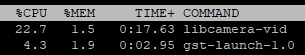
\includegraphics[width=\textwidth]{fig/gstreamer-libcamera_top_v2.png}
        \caption{libcamera-vid piping video to gstreamer}
\end{figure}

\begin{figure}[!htb]
    \centering
    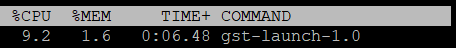
\includegraphics[width=\textwidth]{fig/gstreamer-raspicam_top_v2.png}
    \caption{v4l2src (RaspiCam) feeding video to gstreamer}
\end{figure}

Unfortunately, the newest Pi Camera Module v3 is not compatible with the legacy RaspiCam drivers.

\section{Hardware Acceleration for ML Inference}

\subsection{Google Coral TPU}
The Coral TPU is a compact, power-efficient chip designed by Google to accelerate TensorFlow Lite models on devices. It enables rapid machine learning processing, enhances data privacy, and eliminates the need for continuous internet connectivity. Developers can achieve high-performance machine learning inferencing, making it an ideal choice for applications like computer vision and natural language processing in various edge devices. \cite{CoralTPU}

\begin{figure}[h]
    \centering
    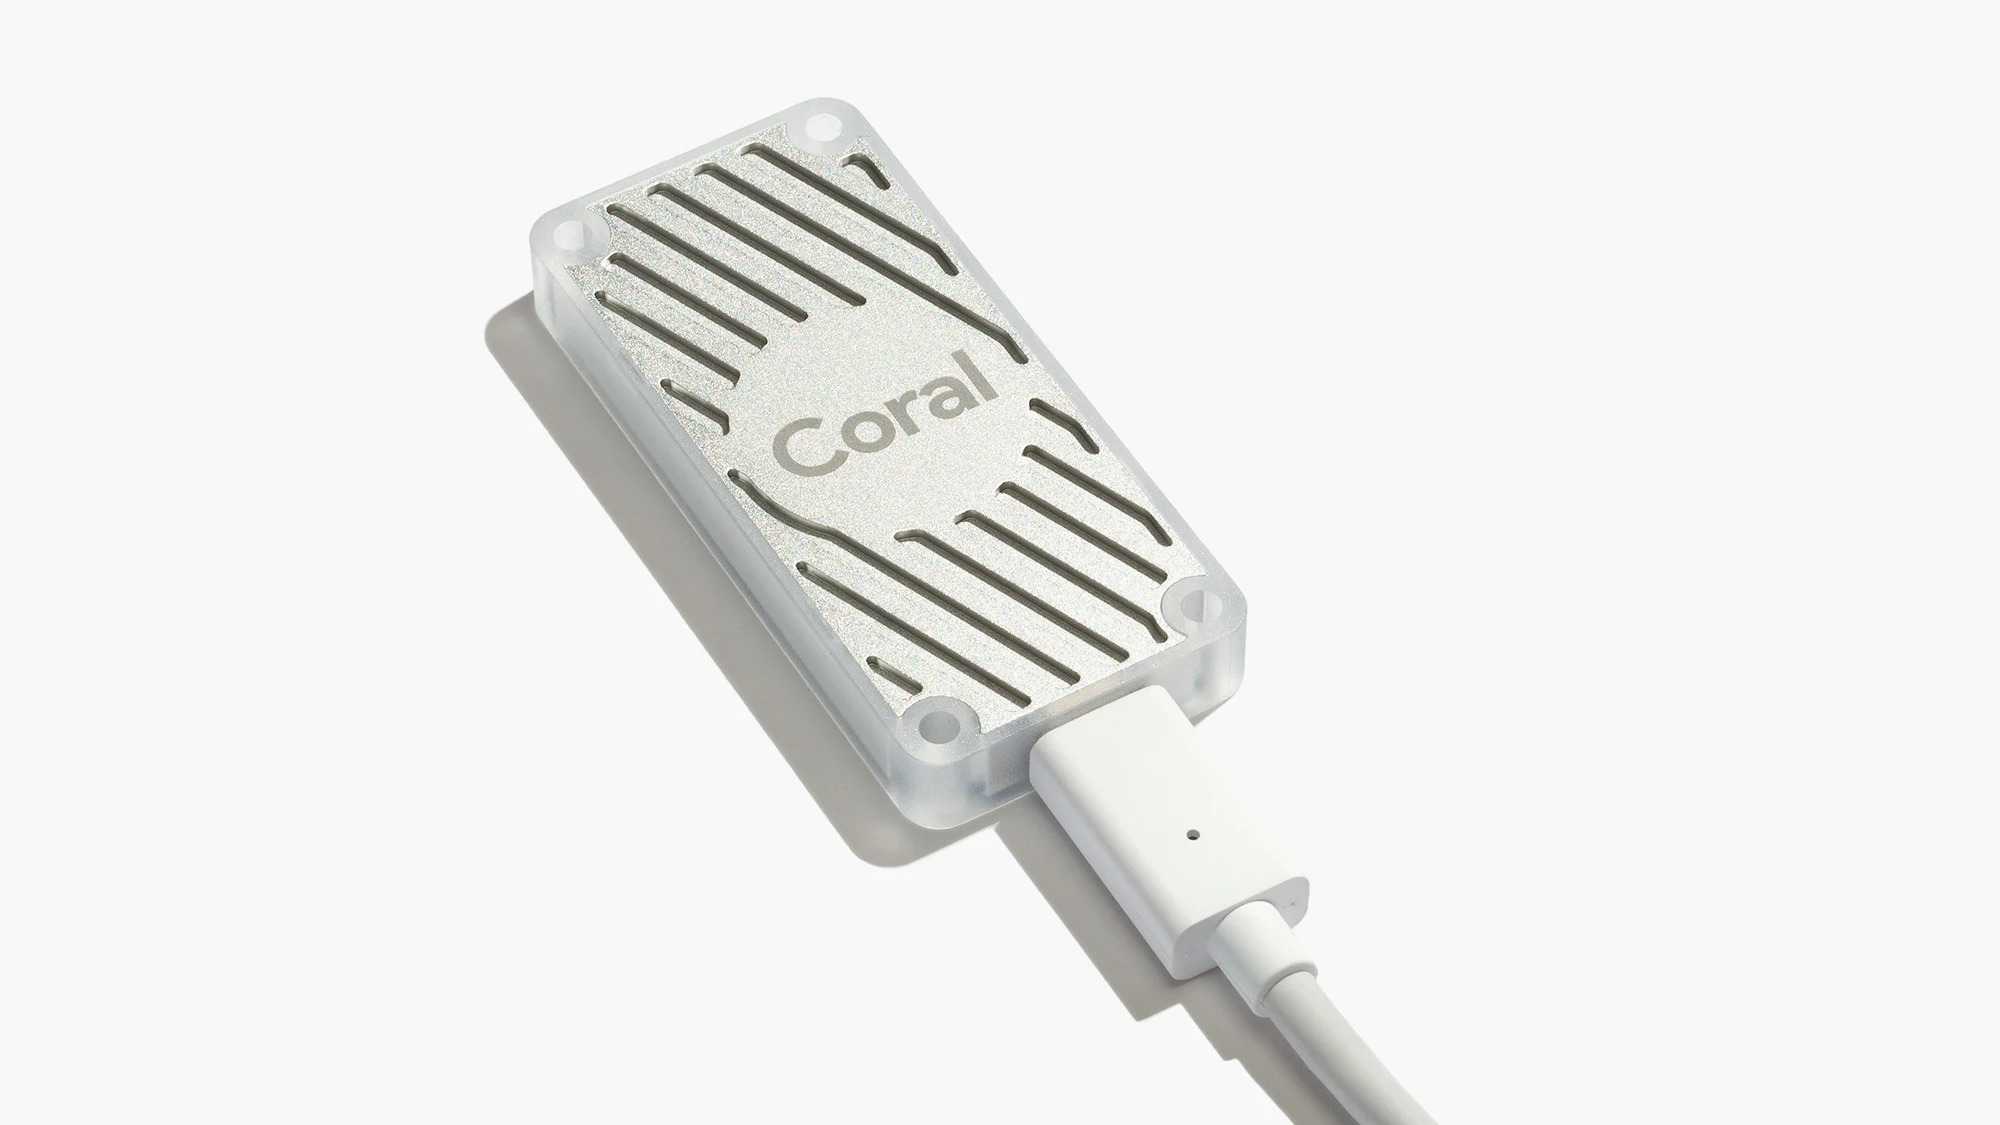
\includegraphics[scale=0.15]{fig/Coral TPU.jpg}
    \caption{Coral USB accelerator \cite{CoralTPU_bilde}}
\end{figure}

\section{Flight controller}
\label{fc}

When choosing flight controller (FC) board(s) for the hardware stack of our test-solution architectures we tend to mainly look at processor speed and flash memory in relation to form factor and weight as well as the availability in local retail shops. The boards' sensor and connectivity options are aspects we deem less relevant for our research project.

F1, F3, F4, G4, F7, and H7 are the different STM32 processors (aka MCU – Micro Controller Unit). The processor is the brain of a flight controller (FC), similar to the CPU in a computer.

There are currently 11 series of STM32 MCU, from faster to slower processing speeds they are: H7, F7, G4, F4, F3, F2, F1, F0, L4, L1, and L0. \cite{comparison-FC}

We decided to go for a single FC to be used in all the hardware stacks of our test-solution architectures of the latest and greatest generation FC that employs the fastest H7-generation microcontroller unit (MCU) with 2 MB of flash memory. This ensures the drone can run very smoothly and has sufficient flash memory to support any firmware with a full set of features.

\begin{table}
\begin{tabular}{ | >{\raggedright}p{\dimexpr 0.26\linewidth-2\tabcolsep} |
                   >{\raggedleft}p{\dimexpr 0.25\linewidth-2\tabcolsep} |
                   >{\raggedleft}p{\dimexpr 0.25\linewidth-2\tabcolsep} |
                   >{\raggedleft\arraybackslash}p{\dimexpr 0.24\linewidth-2\tabcolsep} | } \hline

\bfseries{Processor}        & \centering\bfseries{Processor Speed}    & \centering\bfseries{Flash Memory}   & \centering\arraybackslash\bfseries{SRAM} \\\hline
\bfseries{F0 (STM32F051)}   & 48MHz                         & 256KB                     & 32KB  \\\hline
\bfseries{F1 (STM32F103)}   & 72MHZ                         & 128KB                     & 96KB  \\\hline
\bfseries{F3 (STM32F303)}   & 72MHz                         & 256KB                     & 80KB  \\\hline
\bfseries{F4 (STM32F405)}   & 168MHz                        & 1MB                       & 192KB \\\hline
\bfseries{F4 (STM32F411)}   & 100MHz                        & 512KB                     & 128KB \\\hline
\bfseries{G4 (STM32G491)}   & 170MHz                        & 512KB                     & 128KB \\\hline
\bfseries{F7 (STM32F745)}   & 216MHz                        & 1MB                       & 320KB \\\hline
\bfseries{F7 (STM32F722)}   & 216MHz                        & 512KB                     & 256KB \\\hline
\bfseries{F7 (STM32F765)}   & 216MHz                        & 2MB                       & 512KB \\\hline
\bfseries{H7 (STM32H743)}   & 480MHz                        & 2MB                       & 1MB   \\\hline

\end{tabular}
\caption{Comparison table for microcontroller unit (MCU) \protect\cite{comparison-FC}}
\end{table}

We decided we wanted to go for a single FC for the hardware stacks of our test-solution architectures. Employing the "STM32H743" MCU, it ensures the drone can run very smoothly and has sufficient flash memory to support any firmware with a full set of features.

We ended up going for a MATEKSYS Flight Controller H743-SLIM \cite{MateksysH743-SLIM} as it fulfills our criteria and could be readily ordered at the Norwegian online store "elefun.no".

\begin{figure}[!htb]
    \centering
    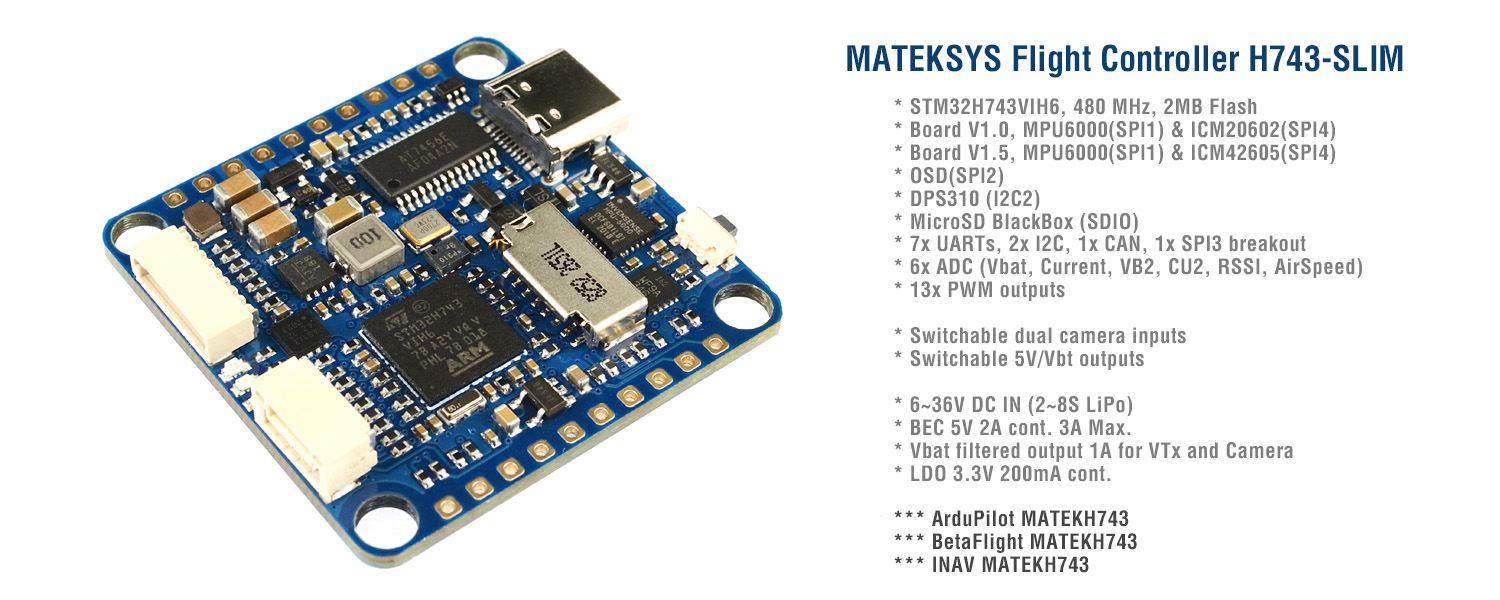
\includegraphics[width=\textwidth]{fig/H743-SLIM_1.jpg}
    \caption{Showcase of MATEKSYS H743-SLIM, from mateksys.com \protect\cite{MateksysH743-SLIM}}
\end{figure}

\newpage


% Deaktiverer denne:
\iffalse
\subsection{PID controller for autonomous flying}

A proportional–integral–derivative controller (PID controller or three-term controller) is a control loop mechanism employing feedback that is widely used in industrial control systems and a variety of other applications requiring continuously modulated control. A PID controller continuously calculates an error value e(t) as the difference between a desired setpoint (SP) and a measured process variable (PV) and applies a correction based on proportional, integral, and derivative terms (denoted P, I, and D respectively), hence the name. \cite{wiki-PID-controller}

\begin{figure}[!htb]
    \centering
    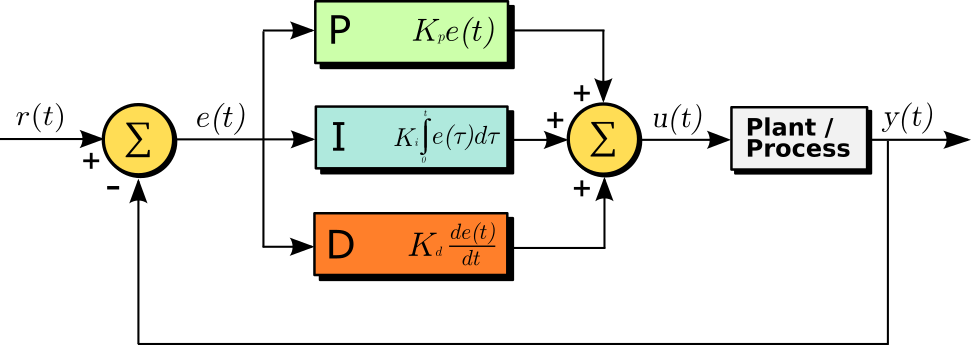
\includegraphics[width=\textwidth]{fig/PID-controller.png}
    \caption{PID controller, from wikipedia.org \protect\cite{wiki-PID-controller}}
\end{figure}

We believe in this stage of the project that it's possible to employ a PID controller program for real-time calculation of the drone's desired action while fed input data from an object detection program running in parallel.
The PID controller program will then generate MAVLink messages to somehow control the drone. This can possibly be done through MAVLink's Manual Control Protocol.
\fi

%\chapter{Software}
%\label{ch:software}
%\title{Software}

\section{Operating System Architecture}
A key element in our research is to make sure our results are predictable and reproducible, and in order to achieve this we need to control for variables as much as possible. Our plan is to create a common platform across all hardware and software configuration, this is so that any variations on the operating system level is negated. 
The hardware we are working on is best supported on Linux, where the kernel and driver architecture is rapidly evolving, and the difference between different versions can be very noticeable.

\section{Nvidia Jetpack}
The Nvidia Jetpack SDK is a package of tools, libraries, and frameworks designed to simplify the development and deployment of AI applications on the Nvidia Jetson platform. Jetpack SDK offers developers a range of resources and tools.
\\
Operating system - An optimized Linux-based operating system for Jetson platforms.
\\
CUDA Toolkit – A set of tools and libraries for developing GPU-accelerated applications.
\\
cuDNN library – A deep learning library that provides GPU-accelerated primitives for deep learning frameworks.
\\
TensorRT – A high-performance deep learning inference optimizer and runtime library.

\section{ROS2}
ROS2 is an open-source robotic middleware that offers a comprehensive framework for robot control and interaction by facilitating hardware abstraction, device management, and inter-process communication. It enables a distributed network of processes that can work together seamlessly, employing different communication methods to ensure efficient and effective robot operation. 

\section{TensorRT}
TensorRT is an NVIDIA-developed high-performance deep learning inference library, designed to accelerate neural network computations on NVIDIA GPUs. This tool optimizes and compiles models from major deep learning frameworks, such as TensorFlow or PyTorch, into efficient CUDA code. By utilizing kernel fusion, layer auto-tuning, and precision calibration, TensorRT significantly enhances inference latency and throughput, enabling real-time performance for various AI applications.

\section{Tensorflow Lite}
TensorFlow Lite is a toolset designed for running machine learning models on devices like mobile phones and embedded systems. It's optimized for on-device performance, focusing on low latency, privacy, reduced model size, and efficient power consumption. The framework supports multiple platforms, including Android, iOS, embedded Linux, and microcontrollers, making it versatile for various applications. 

\section{Docker}
Docker is a platform that allows you to easily create, deploy, and run applications in a containerized environment. Containers are lightweight and portable, and they allow you to package up all of the dependencies and configurations that your application needs to run.\\

With Docker, you can create a container image that includes your application code, libraries, and system tools, and then deploy that image to any Docker-enabled environment, whether it's your local machine or a cloud-based server.\\

Docker provides a number of benefits, including:\\

Portability: Docker containers can be run on any Docker-enabled system, regardless of the underlying operating system or hardware.\\

Isolation: Containers provide a level of isolation between applications, so you can run multiple applications on the same system without worrying about conflicts or dependencies.\\

Consistency: By packaging all of your application's dependencies and configurations into a container image, you can ensure that your application runs consistently across different environments.\\

Efficiency: Containers are lightweight and can be started and stopped quickly, which makes them ideal for scaling and resource optimization.\\

Overall, Docker is a powerful tool for simplifying application deployment and management, and it's widely used in both development and production environments

\section{YOLO (You Only look Once)}
YOLO (You Only Look Once) is a real-time object detection system that is known for its speed and accuracy. It is based on a single neural network that simultaneously predicts multiple bounding boxes and class probabilities for each box. Unlike traditional object detection methods that use a sliding window approach, YOLO processes an entire image in a single forward pass, making it highly efficient for real-time applications.
YOLO divides an image into a S x S grid and predicts bounding boxes and class probabilities for each grid cell. The model then combines these predictions to produce the final object detection output. 
The system has undergone several revisions and improvements, with the latest version being YOLOv8.

\section{OpenCV}
OpenCV is an open-source computer vision and machine learning library that is used to analyze and manipulate visual data in real-time. It is used for a wide range of applications, including image and video processing, facial recognition, object detection, and tracking. OpenCV provides a set of powerful tools and algorithms which makes it easy to work with images and videos, including tools for image filtering, feature detection, and machine learning. It is widely used in industries like robotics, surveillance, and automotive. OpenCV is particularly useful with Python due to its ease of use making it a popular choice for developers and researchers who want to work with computer vision applications.

OpenCV has numerous advantages and some of them are:
\begin{itemize}
\item Open-source and free to use and modify 
\item Supported by a vast community of developers 
\item Highly efficient with optimized algorithms for real-time visual data 
processing
\end{itemize}

However, there are some drawbacks to using OpenCV including: 
\begin{itemize}
\item Steep learning curve, especially for those new to computer vision and machine learning 
\item Somewhat complex to integrate with certain systems. Depending on the specific requirements and capabilities of the system being used
\item Primarily a low-level library, challenging to use for higher-level applications 
\end{itemize}
Despite these limitations, OpenCV remains a powerful and versatile tool for visual data analysis and manipulation.

There are different techniques used in OpenCV and some of them are: 

\textbf{Blob detection:}

In OpenCV, "blobs" refer to groups of connected pixels that share similar characteristics, such as color or texture. Blob detection is a common computer vision technique used for image segmentation, object tracking, and feature extraction

\textbf{Contour detection:} 

Contours refer to the boundaries of objects in an image or video. They are often used for object detection, recognition, and classification. In OpenCV, contours can be found using the "findContours()" function, which detects and extracts the boundaries of objects in an image.

%More information about techniques used in OpenCV can be found here 

\section{Computer vision}
“Computer vision is a field of artificial intelligence (AI) that enables computers and systems to derive meaningful information from digital images, videos and other visual inputs — and take actions or make recommendations based on that information. If AI enables computers to think, computer vision enables them to see, observe and understand.” \cite{Computer-vision} 

Computer vision is a broad field and includes a wide range of techniques and applications. in this thesis, we will use two of them, object detection and blob detection.

%Skal denne slettes?
\subsection{Blob detection}
Blob detection is considered one of the traditional techniques in computer vision. It relies on simpler image processing methods rather than more advanced machine learning approaches. It detects areas or "blobs" in an image that differs from the surroundings. This can be color, shape, or size.
%Hvor hører denne hjemme nå?
\subsection{Object detection}
Object detection is a more advanced technique of computer vision. Widely-used deep learning methods that employ convolutional neural networks (CNNs), such as SSD and YOLO, can automatically learn to identify objects in images. You have two options when training a model: you can either create a custom model from scratch or employ transfer learning. Transfer learning involves using a pre-trained model and adapting it with your own dataset to suit your specific needs.


\section{Qualisys}

Qualisys motion capture systems can be used for accurately determining the position of the drone. The system provides precise real-time 6DOF (6 degrees of freedom) positioning data, allowing you to track and analyze the drone's position in the room or any environment. 

%\chapter{Risk Analysis}
%\label{ch:risikoanalyse}
%\title{Risiko}

\section{Risk Analysis}

Risk analysis is an ongoing process that continuously evaluates risk throughout the project's lifecycle. It is the responsibility of the risk manager to ensure that this process takes place regularly and consistently during the project. This is crucial because it raises awareness among both us and our customers about potential risks and vulnerabilities, encourages necessary improvements, and facilitates necessary changes. Such analysis can help the risk manager identify new risks and changes that require attention along the way. \cite{Risk1}

After identifying risks, it is essential to prioritize them based on their probability and severity. Moreover, measures should be put in place to manage them effectively if they occur. While everyone on the team should participate in assessing the project's risks, the risk manager will be primarily responsible for ensuring quality assurance. \cite{Risk2}

A risk analysis was conducted for our project, wherein we identified both internal and external risks. Internal risks are linked with factors that are under our control, whereas external risks are associated with factors that lie beyond our control.\cite{RiskInternalExternal} A few examples of these risks are:\\



Internal risks:
\begin{itemize}
    \item If multiple get sick at the same time? 
    \item If someone suddenly wants to quit
\end{itemize}
External risks:
\begin{itemize}
    \item New nationwide pandemic
    \item Component availability with regard to a global shortage
\end{itemize}

After identifying the risks at this stage, we evaluate their potential consequences and determine the appropriate measures that can be taken if they occur. To gain a better overview, we record the risks in a table that includes a unique code, a description of the risk event, recommended measures, probability (P), consequence (C), and priority. Below is a comprehensive overview of both internal and external risks:


\begin{figure}
\centering
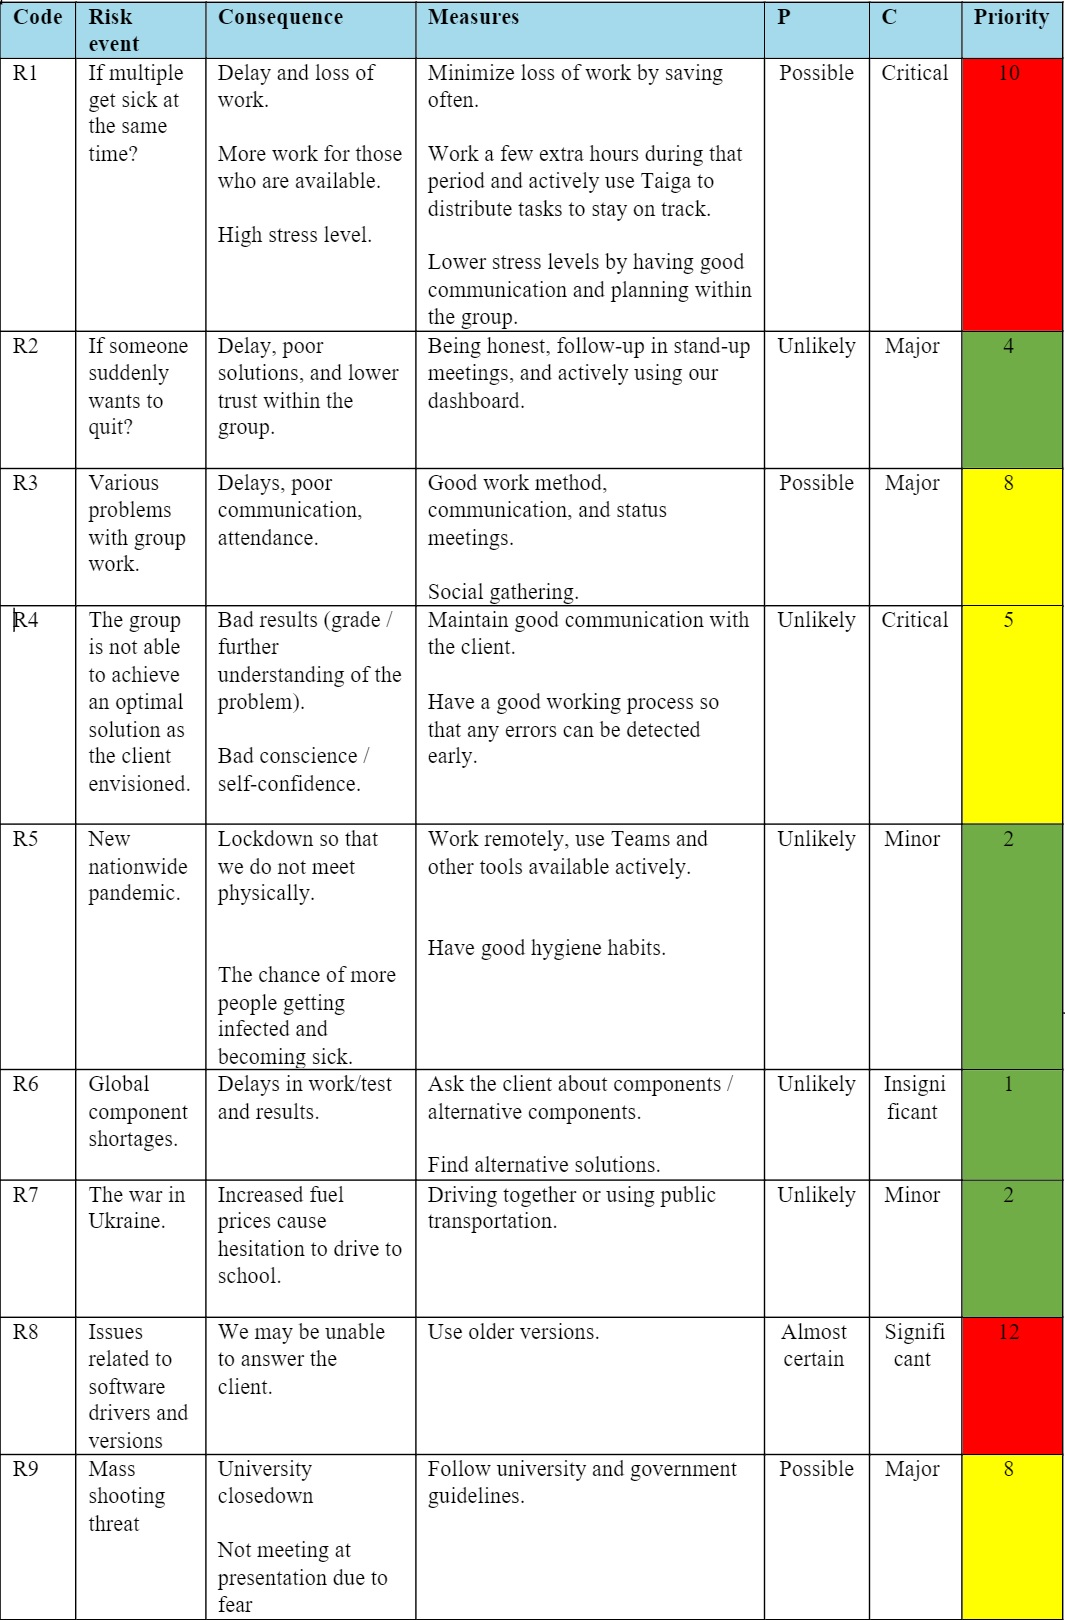
\includegraphics[width=0.85\linewidth]{fig/RisikoTabell.jpg}
\caption{Risk table}
\label{fig:yourlabel}
\end{figure}

\newpage

The prioritization of these risks was determined by evaluating their consequence and probability using the risk matrix:

\begin{figure}[h!]
\centering
\includegraphics[width=0.85\linewidth]{fig/Risk matrix.jpg}
\caption{Risk Matrix \cite{RiskMatrix}} 
\label{fig:yourlabel}
\end{figure}




%\chapter{Algorithms}
%\label{ch:algorithms}
%
\section{Blob detection.v1}

Since we use the Raspberry Pi Camera Module v3 and not a depth camera, we need to find a way to find the distance to a known object. We ended up using OpenCV and cvzone. Our approach involves detecting a specific color in the video frames, identifying the contours of the detected object, and then calculating the distance based on the object's apparent size in the image.

First, we import the necessary packages for image processing, numerical operations, and color detection:

\begin{lstlisting}[language=PythonPlus]
import cv2
import cvzone
from cvzone.ColorModule import ColorFinder
import numpy as np
\end{lstlisting}

We create a VideoCapture object (OpenCV) to read video frames from the camera \cite{OpenCVDoc}, and set the capture dimensions to 640x480 pixels \cite{OpenCVDoc}:

\begin{lstlisting}[language=PythonPlus]
cap = cv2.VideoCapture(0)
cap.set(3, 640)
cap.set(4, 480)
\end{lstlisting}

Next, we create a ColorFinder object (cvzone) with automatic color range update turned off \cite{CVzoneDoc}, and define the color range for detection (using predetermined HSV values):

\begin{lstlisting}[language=PythonPlus]
myColorFinder = ColorFinder(False)
hsvVals = {'hmin': 97, 'smin': 21, 'vmin': 23, 'hmax': 125, 'smax': 255, 'vmax': 193}
\end{lstlisting}

In a continuous loop, we read the video frames from the camera (OpenCV) \cite{OpenCVDoc}, detect the specified color range in the image using the ColorFinder object (cvzone) \cite{CVzoneDoc}, and find the contours in the binary mask (cvzone) \cite{CVzoneDoc}:

\begin{lstlisting}[language=PythonPlus]
while True:
    success, img = cap.read()
    imgColor, mask = myColorFinder.update(img, hsvVals)
    imgContour, contours = cvzone.findContours(img, mask)
\end{lstlisting}

When contours are detected, we extract data from the first contour (assumed to be the object of interest) and calculate the distance to the object based on its apparent size in the image. We use the real-world dimensions of the object (in this case, a tennis ball with a width of 6.5 cm) and the camera's focal length to compute the distance:

\begin{lstlisting}[language=PythonPlus]
if contours:
    data = contours[0]['center'][0], h - contours[0]['center'][1], int(contours[0]['area'])
    
    f = 535  # focal length of the camera
    W = 6.5  # real-world width of the tennis ball

    w = np.sqrt(contours[0]['area']/np.pi) * 2  # width of the tennis ball in the image
    d = (W * f) / w  # calculate the distance

    print(d)
\end{lstlisting}

Finally, we display the distance in centimeters on the image (cvzone) \cite{CVzoneDoc} and stack the original image, detected color image, binary mask, and contour image for visualization (cvzone) \cite{CVzoneDoc} this is done for testing purpose:

\begin{lstlisting}[language=PythonPlus]
cvzone.putTextRect(img, f'depth: {int(d)} cm', (contours[0]['center'][0] - 75, contours[0]['center'][1] - 50), scale= 2)
imgStack = cvzone.stackImages([img, imgColor, mask, imgContour], 2, 0.5)
cv2.imshow("Image", imgStack)
cv2.waitKey(1)
\end{lstlisting}

This approach is suitable for objects with known dimensions and relatively uniform color distribution. This testing was used with simple color detection. We can use this function to use the contours of trained models to find the distance as well. \newpage

\section{Blob detection.v2}

This code uses OpenCV \cite{OpenCVDoc} and cvzone \cite{CVzoneDoc} to track and measure the distance of 3 tennis-sized balls with different colors in a live video feed from a webcam.

First, we import the necessary packages:
\begin{lstlisting}[language=PythonPlus]
import cv2 as cv
from cvzone.FPS import FPS
import imutils
import math
import numpy as np
\end{lstlisting}

This function \verb|calculateDistance| is used to calculate the distance from the camera to the object based on the radius of the object in pixels. This calculation is based on similar triangles and the field of view of the camera.
\begin{lstlisting}[language=PythonPlus]
# Function to calculate distance from the object based on its radius in pixels
def calculateDistance(ballRadius_px):
    return int(faktor / ballRadius_px)
\end{lstlisting}

This function \verb|detect_colored_object| uses color-based filtering and shape-based detection to identify and locate the colored ball in the video frame \cite{ColoredObject}. The function uses color filtering to create a mask for pixels within the defined color range and applies the Hough Transform function \cite{OpenCVHoughCircle} on a blurred grayscale version of the frame to detect circles. If a detected circle's center lies within the color mask, the function returns the circle's coordinates and radius\cite{CircleDetection}.
\begin{lstlisting}[language=PythonPlus]
# Function to detect a colored object within a given color range and size
def detect_colored_object(colorLower, colorUpper, min_radius, max_radius):
    mask = cv.inRange(hsv, colorLower, colorUpper)
    
    # Erode the mask to remove noise & Dilate the mask to fill gaps
    mask = cv.erode(mask, None, iterations=2)
    mask = cv.dilate(mask, None, iterations=2)
    
    # Convert the frame to grayscale and apply median blur
    gray = cv.cvtColor(frame, cv.COLOR_BGR2GRAY)
    gray = cv.medianBlur(gray, 5)

    # Detect circles using the Hough transform
    circles = cv.HoughCircles(gray, cv.HOUGH_GRADIENT, 1, 20, param1=100, param2=30,
                              minRadius=min_radius, maxRadius=max_radius)

    # Check if any circles were detected
    if circles is not None:
        circles = np.uint16(np.around(circles))

        for circle in circles[0, :]:
            x, y, radius = circle

            # Check if the circle's center is within the mask's boundaries
            if 0 <= x < mask.shape[1] and 0 <= y < mask.shape[0] and mask[y, x] > 0:
                return (x, y, radius)
    return None
\end{lstlisting}

The function \verb|display_object_info| visualizes \cite{OpenCVDisplay} details such as a circle around the detected object, x, and y coordinates, and estimated distance on the video frame. 
\begin{lstlisting}[language=PythonPlus]
# Function to display information about the detected object on the frame
def display_object_info(frame, x, y, radius, distance, color, text_offset):
    if x is not None and y is not None:
        # Draw a circle around the detected object
        cv.circle(frame, (x, y), radius, color, 2)
        
        # Display the coordinates x and y
        coordinates_text = f"X: {x}, Y: {y}"
        
        # Display the distance text
        distance_text = f"Distance: {distance} cm"
        
        # Put the coordinate text on the frame
        cv.putText(frame, coordinates_text, (x + 10, y), cv.FONT_HERSHEY_SIMPLEX, 0.5, color, 2)
        
        # Put the distance text on the frame
        cv.putText(frame, distance_text, (22, 70 + text_offset), cv.FONT_HERSHEY_SIMPLEX, 0.5, color, 2)
\end{lstlisting}

The \verb|ballRadius| is a variable indicating the radius of the tennis ball, the \verb|cameraFOV| is the camera's field of view, and lastly, the \verb|faktor| is a calculation parameter \cite{CircleParameters} used to determine the distance of the object from the camera. 
\begin{lstlisting}[language=PythonPlus]
ballRadius = 3.25   # cm (radius of the ball)
cameraFOV = 62.2    # degrees (field of view of the camera)
faktor = (1280 / 2) * (ballRadius / math.tan(math.radians(kameraFOV / 2))) # Pixels from center to edge divided by minimum distance from the lens
\end{lstlisting}

For each color, the program attempts to detect an object of that color in the frame \cite{OpenCVIterate}. If an object is found, its properties (coordinates, distance) are updated in the color dictionary. The updated information is then displayed \cite{OpenCVDisplay} on the frame. This process repeats for each frame, enabling real-time tracking.
\begin{lstlisting}[language=PythonPlus]
# Main loop
while True:
    (grabbed, frame) = videoCap.read() # Read a frame from the video capture
    fps, img = fpsreader.update(frame, color=(255, 0, 0)) # Update the FPS overlay on the frame
    frame = imutils.resize(frame, width=1280) # Resize the frame
    hsv = cv.cvtColor(frame, cv.COLOR_BGR2HSV) # Convert the frame to HSV format

    # Initialize x, y, and ballRadius_px values for each color
    for color_info in colors.values():
        color_info['x'] = None
        color_info['y'] = None
        color_info['ballRadius_px'] = None

    # Iterate through the defined colors and detect objects
    for idx, (color_name, color_info) in enumerate(colors.items()):
        # Call the detect_colored_object function to find objects in the frame
        obj = detect_colored_object(color_info['lower'], color_info['upper'], color_info['min_radius'],
                                    color_info['max_radius'])

        if obj: # If an object is detected, get the coordinates and radius, distance
            x, y, ballRadius_px = obj
            distance = kalkulerDistanse(ballRadius_px) 
            
            # Update the color_info dictionary with the new values
            color_info['x'] = x
            color_info['y'] = y
            color_info['ballRadius_px'] = ballRadius_px
            color_info['distance'] = distance
\end{lstlisting}

The \verb|display_object_info| function visually \cite{OpenCVDisplay} presents data about the detected object on the video feed.
\begin{lstlisting}[language=PythonPlus]
# Display information about the detected object on the frame
        display_object_info(frame, color_info['x'], color_info['y'], color_info['ballRadius_px'],
                            color_info.get('distance'), color_info['color'], color_info['text_offset'])

    cv.imshow("Frame", frame)  # Show the frame
\end{lstlisting}
Referring back to the discussion in the 'Configuration 4 Journey' section, it was clear that the computational demands of our program far exceeded the capabilities of the hardware in use, given that the development and testing were conducted on a high-end laptop utilizing a webcam. As a result, we needed to revisit our approach and develop Blob detection.v3. 

\section{Blob detection.v3}
By simplifying and
removing some of the more computationally intense functionalities from the program we developed Blob detection.v3.

First, we import the necessary packages:
\begin{lstlisting}[language=PythonPlus]
import cv2
import cvzone
from cvzone.ColorModule import ColorFinder
from cvzone.FPS import FPS
import numpy as np
\end{lstlisting}

The \verb|is_circle| function checks if a shape is circular enough to be considered a circle. If the shape is "round enough" (the roundness is more than the given threshold, which is set to 0.6), it filters out shapes that are not "round enough".
\begin{lstlisting}[language=PythonPlus]
# Function to check if a contour is a circle
def is_circle(cnt, threshold=0.6):
    area = cv2.contourArea(cnt) # Compute the area of the contour
    perimeter = cv2.arcLength(cnt, True) # Compute the perimeter of the contour
    if perimeter == 0: # If the perimeter is zero, it cannot be a circle, return False
        return False
    circularity = 4 * np.pi * area / (perimeter * perimeter) # Calculate the circularity of the contour
    return circularity >= threshold
\end{lstlisting}


Next, we create a \verb|ColorFinder| object (cvzone) with automatic color range update turned off \cite{CVzoneDoc}, and define the color range for detection using predetermined HSV (Hue, Saturation, Value) values:
\begin{lstlisting}[language=PythonPlus]
myColorFinder: ColorFinder = ColorFinder(False)

# Define the HSV color range for blue, green and orange
hsvValsBlue = {'hmin': 105, 'smin': 168, 'vmin': 119, 'hmax': 111, 'smax': 255, 'vmax': 255} #blue
hsvValsGreen = {'hmin': 76, 'smin': 29, 'vmin': 132, 'hmax': 97, 'smax': 124, 'vmax': 255} #green
hsvValsOrange = {'hmin': 0, 'smin': 120, 'vmin': 120, 'hmax': 20, 'smax': 255, 'vmax': 255} #orange
\end{lstlisting}

Each frame from the camera (OpenCV) \cite{OpenCVDoc}, is read and processed for frame rate, which at first is analyzed to find areas that match the color profiles defined for blue, green, and orange in HSVvalues\cite{CVzoneDoc}, and then analyze these colored areas further to identify contours in those regions. These contours are checked for circularity using the \verb|is_circle| function, thereby extracting contours that are likely to be circles.  
\begin{lstlisting}[language=PythonPlus]
    # Update the color detection for blue, green and orange
    imgColorBlue, mask = myColorFinder.update(img, hsvValsBlue)
    imgColorGreen, maskRed = myColorFinder.update(img, hsvValsGreen)
    imgColorOrange, maskOrange = myColorFinder.update(img, hsvValsOrange)

    # Find contours in blue, green and orange color mask 
    imgContourBlue, contours = cvzone.findContours(img, mask)
    imgContourGreen, contoursRed = cvzone.findContours(img, maskRed)
    imgContourOrange, contoursOrange = cvzone.findContours(img, maskOrange)

    # Filter contours that are circles
    circular_contours_blue = [cnt for cnt in contours if is_circle(cnt['cnt'])]
    circular_contours_green = [cnt for cnt in contoursRed if is_circle(cnt['cnt'])]
    circular_contours_orange = [cnt for cnt in contoursOrange if is_circle(cnt['cnt'])]
\end{lstlisting}

Processes and displays the depth, x-position, and y-position for each detected ball. It iterates over three lists containing circular contours for each color, and checks if there are circular contours detected. If so, it selects the first contour and calculates the depth of the ball using its area and predefined values for focal length and ball width \cite{distanceobject}. It then prints the color of the ball and its depth.
\begin{lstlisting}[language=PythonPlus]
# Process and display depth, x, and y position for each ball
    for color, circular_contours_list in zip(['blue', 'green', 'orange'],
                                             [circular_contours_blue, circular_contours_green, circular_contours_orange]):
        if circular_contours_list:
            cnt = circular_contours_list[0]
            data = cnt['center'][0], h - cnt['center'][1], int(cnt['area'])

            f = 474 #focal length of the camera
            W = 6.5 # real-world width of the tennis ball
            w = np.sqrt(cnt['area'] / np.pi) * 2 # width of the tennis ball in the image
            d = (W * f) / w # calculate the distance
            print(f"{color}: {d}")
\end{lstlisting}

The depth is displayed using \verb|cvzone.putTextRect| function\cite{CVzoneDoc} which adds the text "depth: {int(d)} cm" to the \verb|imgContourBlue| image. The x and y position is also displayed using \verb|cvzone.putTextRect|. \verb|ImgStack| is a stack of the original image, color image with a blue mask, binary mask, and contour image, which is then shown with \verb|cv2.imshow|\cite{CVzoneDoc}.
\begin{lstlisting}[language=PythonPlus]
            # Display depth on the frame
            cvzone.putTextRect(imgContourBlue, f'depth: {int(d)} cm',
                               (cnt['center'][0] - 75, cnt['center'][1] - 50), scale=2)
            # Display x and y position on the frame with more space between depth and position
            cvzone.putTextRect(imgContourBlue, f'x: {cnt["center"][0]}, y: {cnt["center"][1]}',
                               (cnt['center'][0] - 75, cnt['center'][1] - 10), scale=1.5)

    imgStack = cvzone.stackImages([img, imgColorBlue, mask, imgContourBlue], 2, 0.5)
    cv2.imshow("Image", imgStack)
\end{lstlisting}
This version offered a significant improvement in frame rate performance and detection and was further tested on Rasberry Pi. 

\newpage


\newpage
\section{Blob Detection.v3 Evaluation} \label{C4evaluation}

We first import the necessary packages to enable image processing, numerical operations, and color detection:

\begin{lstlisting}[language=PythonPlus]
import cv2
import cvzone
from cvzone.ColorModule import ColorFinder
import numpy as np
import xml.etree.ElementTree as ET
import os
import csv
\end{lstlisting}

The function \verb|is_circle| is created to check if a detected contour is circular or not. We calculate the area and the perimeter of the contour and use these values to calculate the circularity. A threshold is set to determine whether the contour is circular or not:

\begin{lstlisting}[language=PythonPlus]
def is_circle(cnt, threshold=0.6):
    area = cv2.contourArea(cnt)
    perimeter = cv2.arcLength(cnt, True)
    if perimeter == 0:
        return False
    circularity = 4 * np.pi * area / (perimeter * perimeter)
    return circularity >= threshold
\end{lstlisting}

The \verb|parse_label| function is designed to parse label information from an XML file. It extracts the name and bounding box coordinates of an object:

\begin{lstlisting}[language=PythonPlus]
def parse_label(xml_file):
    tree = ET.parse(xml_file)
    root = tree.getroot()

    label = {}
    for obj in root.findall('object'):
        name = obj.find('name').text
        box = obj.find('bndbox')
        xmin = int(box.find('xmin').text)
        xmax = int(box.find('xmax').text)
        ymin = int(box.find('ymin').text)
        ymax = int(box.find('ymax').text)
        
        label[name] = [(xmin, ymin, xmax, ymax)]
    return label
\end{lstlisting}
\newpage
We create the \verb|calculate_f1_score| function to compute the F1 score given precision and recall:\cite{preandrec}[p. 156]

\begin{lstlisting}[language=PythonPlus]
def calculate_f1_score(precision, recall):
    if precision + recall == 0:  # to avoid division by zero
        return 0
    else:
        f1_score = 2 * (precision * recall) / (precision + recall)
        return f1_score
\end{lstlisting}

Next, we define the \verb|read_image| function that simply reads an image from a given path using the OpenCV function \verb|imread|:

\begin{lstlisting}[language=PythonPlus]
def read_image(image_file):
    return cv2.imread(image_file)
\end{lstlisting}

In the \verb|detect_color| function, we detect colors in an image using a pre-defined HSV value range. We then use cvzone's findContours function to find the contours in the binary mask. A filter is applied to only select contours that pass the is\_circle test:

\begin{lstlisting}[language=PythonPlus]
def detect_color(image):
    myColorFinder = ColorFinder(False)
    #hsvVals = {'hmin': 49, 'smin': 69, 'vmin': 17, 'hmax': 108, 'smax': 255, 'vmax': 181} #green
    #hsvVals = {'hmin': 0, 'smin': 42, 'vmin': 0, 'hmax': 20, 'smax': 186, 'vmax': 219} #red
    hsvVals = {'hmin': 87, 'smin': 78, 'vmin': 0, 'hmax': 114, 'smax': 195, 'vmax': 174} #blue
    imgColor, mask = myColorFinder.update(image, hsvVals)
    imgContour, contours = cvzone.findContours(image, mask)

    circular_contours = [cnt for cnt in contours if is_circle(cnt['cnt'])]

    results = []
    if circular_contours:
        for cnt in circular_contours:
            x, y, w, h = cv2.boundingRect(cnt['cnt'])
            results.append(('blue', (x, y, x+w, y+h)))
    return results
\end{lstlisting}
\newpage
The \verb|calculate_iou| function is designed to compute the Intersection over Union (IoU) between two bounding boxes. This metric is commonly used in computer vision tasks to evaluate the accuracy of object detection models: \cite{IoUdoc}

\begin{lstlisting}[language=PythonPlus]
def calculate_iou(box1, box2):
    x1, y1, w1, h1 = box1
    x2, y2, w2, h2 = box2

    xi1 = max(x1, x2)
    yi1 = max(y1, y2)
    xi2 = min(x1 + w1, x2 + w2)
    yi2 = min(y1 + h1, y2 + h2)

    inter_area = max(xi2 - xi1, 0) * max(yi2 - yi1, 0)

    box1_area = w1 * h1
    box2_area = w2 * h2
    union_area = box1_area + box2_area - inter_area

    return inter_area / union_area if union_area > 0 else 0
\end{lstlisting}
\newpage
We define the \verb|calculate_precision_recall| function to compute precision and recall based on predictions and ground truth data. For each prediction, we calculate the maximum IoU with all ground truth boxes of the same color. If this maximum IoU is greater than or equal to a set IoU threshold, it's considered a true positive; otherwise, it's a false positive. False negatives are counted as those ground truth boxes that don't have any corresponding prediction with an IoU greater than or equal to the threshold:\cite{preandrec}[p. 155-156]

\begin{lstlisting}[language=PythonPlus]
def calculate_precision_recall(predictions, ground_truth, iou_threshold=0.5):
    TP = FP = FN = 0

    for image_predictions, image_ground_truth in zip(predictions, ground_truth):
        for pred_color, pred_box in image_predictions:
            if pred_color in image_ground_truth:
                ious = [calculate_iou(pred_box, truth_box) for truth_box in image_ground_truth[pred_color]]
                max_iou = max(ious) if ious else 0

                if max_iou >= iou_threshold:
                    TP += 1
                else:
                    FP += 1
            else:
                FP += 1

        for truth_color, truth_boxes in image_ground_truth.items():
            if truth_color not in [pred_color for pred_color, _ in image_predictions]:
                FN += len(truth_boxes)
            else:
                for truth_box in truth_boxes:
                    ious = [calculate_iou(pred_box, truth_box) for pred_color, pred_box in image_predictions if pred_color == truth_color]
                    max_iou = max(ious) if ious else 0
                    if max_iou < iou_threshold:
                        FN += 1

    precision = TP / (TP + FP) if TP + FP > 0 else 0
    recall = TP / (TP + FN) if TP + FN > 0 else 0

    return precision, recall
\end{lstlisting}
\newpage
In our main procedure, we define paths to our image and label directories, then sort and pair up the corresponding image and label files:

\begin{lstlisting}[language=PythonPlus]
image_dir = '/home/vaffe/RandomStuff/dataset/valid/blue/'
label_dir = '/home/vaffe/RandomStuff/dataset/valid/blue/labels/'

image_files = sorted(os.listdir(image_dir))
label_files = sorted(os.listdir(label_dir))
\end{lstlisting}

The code processes each image file and corresponding label file one by one. It reads the image, detects the color (our function returns the bounding boxes of detected objects), and parses the XML label file to obtain the ground truth bounding boxes. The predictions and ground truth are stored for later evaluation:

\begin{lstlisting}[language=PythonPlus]
for image_file, label_file in zip(image_files, label_files):
    image_path = os.path.join(image_dir, image_file)
    label_path = os.path.join(label_dir, label_file)

    image = read_image(image_path)
    label = parse_label(label_path)

    prediction = detect_color(image)

    predictions.append(prediction)
    ground_truths.append(label)

    print('Predicted: ', prediction)
    print('Ground Truth: ', label)

\end{lstlisting}

Finally, we calculate precision, recall, and F1 score, which are commonly used metrics to evaluate the performance of object detection models:

\begin{lstlisting}[language=PythonPlus]
precision, recall = calculate_precision_recall(predictions, ground_truths)
f1_score = calculate_f1_score(precision, recall)

print('Precision: ', precision)
print('Recall: ', recall)
print('F1 Score: ', f1_score)
\end{lstlisting}

The precision metric quantifies the number of correct positive predictions made, while recall (also known as sensitivity) quantifies the number of correct positive results divided by the number of all relevant samples (all samples that should have been identified as positive). The F1 Score is the harmonic mean of precision and recall and provides a single score that balances both the concerns of precision and recall in one number. \cite{preandrec}[p. 155-156]


%References:

%[1] OpenCV VideoCapture. Retrieved from https://docs.opencv.org/master/d8/dfe/classcv_1_1VideoCapture.html

%[2] OpenCV VideoCapture::set. Retrieved from https://docs.opencv.org/master/d8/dfe/classcv_1_1VideoCapture.html#aa6480e6972ef4c00d74814ec841a2939

%[3] Cvzone. (02.22). ColorModule. Retrieved from  https://github.com/cvzone/cvzone/blob/master/cvzone/ColorModule.py

%[4] Cvzone. (02.22). findContours. Retrieved from https://github.com/cvzone/cvzone/blob/master/cvzone/Utils.py#L81

%[5] Cvzone. (02.22). putTextRect. Retrieved from https://github.com/cvzone/cvzone/blob/master/cvzone/Utils.py#L145

%[6] Cvzone. (02.22). stackImages. Retrieved from https://github.com/cvzone/cvzone/blob/master/cvzone/Utils.py#L12

\chapter{Config4 Source code}
\section{Blob Detection.v1}

\begin{lstlisting}[language=PythonPlus]
import cv2 
import cvzone 
from cvzone.ColorModule import ColorFinder
from cvzone.FPS import FPS  
import numpy as np 

fpsreader = FPS() 
cap = cv2.VideoCapture(0)  
cap.set(3, 640)  
cap.set(4, 480) 

success, img = cap.read()  
h, w, _ = img.shape  

myColorFinder = ColorFinder(False)  
hsvVals = {'hmin': 36, 'smin': 29, 'vmin': 44, 'hmax': 90, 'smax': 150, 'vmax': 187}

while True: 
    success, img = cap.read() 
    fps, img = fpsreader.update(img)
    imgColor, mask = myColorFinder.update(img, hsvVals)
    imgContour, contours = cvzone.findContours(img, mask)  

    if contours:  
        data = contours[0]['center'][0], h - contours[0]['center'][1], int(contours[0]['area'])

        f = 535
        W = 6.5
        w = np.sqrt(contours[0]['area'] / np.pi) * 2
        d = (W * f) / w

        x, y = contours[0]['center'][0], contours[0]['center'][1]

        print("x: ", x)
        print("y: ", y)

        print(fps)

        cvzone.putTextRect(img, f'depth: {int(d)} cm', (contours[0]['center'][0] - 75, contours[0]['center'][1] - 50),
                           scale=2)  
        cv2.putText(img, f'x: {int(x)}, y: {int(y)}', (20, h - 600), cv2.FONT_HERSHEY_SIMPLEX, 1.5, (255, 0, 0),
                    thickness=2)

    imgStack = cvzone.stackImages([img, imgColor, mask, imgContour], 2,
                                  0.5)
    cv2.imshow("Image", imgStack) 

    if cv2.waitKey(1) & 0xFF == ord('q'):
        break
cap.release()
cv2.destroyAllWindows()
\end{lstlisting}

\section{Blob Detection.v2}

\begin{lstlisting}[language=PythonPlus]
import cv2 as cv
from cvzone.FPS import FPS
import imutils
import math
import numpy as np

def calculateDistance(ballRadius_px):
    return int(faktor / ballRadius_px)

def detect_colored_object(colorLower, colorUpper, min_radius, max_radius):
    
    mask = cv.inRange(hsv, colorLower, colorUpper)
    mask = cv.erode(mask, None, iterations=2)
    mask = cv.dilate(mask, None, iterations=2)

    gray = cv.cvtColor(frame, cv.COLOR_BGR2GRAY)
    gray = cv.medianBlur(gray, 5)

    circles = cv.HoughCircles(gray, cv.HOUGH_GRADIENT, 1, 20, param1=100, param2=30,
                              minRadius=min_radius, maxRadius=max_radius)

    if circles is not None:
        circles = np.uint16(np.around(circles))

        for circle in circles[0, :]:
            x, y, radius = circle

            if 0 <= x < mask.shape[1] and 0 <= y < mask.shape[0] and mask[y, x] > 0:
                return (x, y, radius)
    return None

def display_object_info(frame, x, y, radius, distance, color, text_offset):
    if x is not None and y is not None:
       
        cv.circle(frame, (x, y), radius, color, 2)
        coordinates_text = f"X: {x}, Y: {y}"
        distance_text = f"Distance: {distance} cm"

        cv.putText(frame, coordinates_text, (x + 10, y), cv.FONT_HERSHEY_SIMPLEX, 0.5, color, 2)
        cv.putText(frame, distance_text, (22, 70 + text_offset), cv.FONT_HERSHEY_SIMPLEX, 0.5, color, 2)

ballRadius = 3.25   # cm (radius of the ball)
cameraFOV = 62.2    # degrees (field of view of the camera)
faktor = (1280 / 2) * (ballRadius / math.tan(math.radians(kameraFOV / 2)))

colors = {
    'green': {
        'lower': (72, 70, 32), 
        'upper': (99, 244, 107),
        'min_radius': 0, #ex between 0 
        'max_radius': 0, #to ex 60 pixels
        'color': (0, 255, 0), 
        'text_offset': 0, #Distance text position under FPS
    },
    'orange': {
        'lower': (0, 115, 99), 
        'upper': (18, 255, 255), 
        'min_radius': 0,
        'max_radius': 0,
        'color': (0, 102, 255), 
        'text_offset': 20, 
    },
    'red': {
        'lower': (119, 37, 0), 
        'upper': (179, 179, 147), 
        'min_radius': 0,
        'max_radius': 0,
        'color': (0, 0, 255), 
        'text_offset': 40,  
    },
}

fpsreader = FPS() 
videoCap = cv.VideoCapture(0) 
videoCap.set(3, 1280)
videoCap.set(4, 720)

while True:
    (grabbed, frame) = videoCap.read() 
    fps, img = fpsreader.update(frame, color=(255, 0, 0)) 
    frame = imutils.resize(frame, width=1280) 
    hsv = cv.cvtColor(frame, cv.COLOR_BGR2HSV) 

    for color_info in colors.values():
        color_info['x'] = None
        color_info['y'] = None
        color_info['ballRadius_px'] = None

    for idx, (color_name, color_info) in enumerate(colors.items()):
        obj = detect_colored_object(color_info['lower'], color_info['upper'], color_info['min_radius'],
                                    color_info['max_radius'])
        if obj: 
            x, y, ballRadius_px = obj 
            distance = kalkulerDistanse(ballRadius_px) 
            
            color_info['x'] = x
            color_info['y'] = y
            color_info['ballRadius_px'] = ballRadius_px
            color_info['distance'] = distance

        display_object_info(frame, color_info['x'], color_info['y'], color_info['ballRadius_px'],
                            color_info.get('distance'), color_info['color'], color_info['text_offset'])

    cv.imshow("Frame", frame)  
    key = cv.waitKey(1)  
    if key == ord("q"):
        break
\end{lstlisting}

\section{Blob Detection.v3}

\begin{lstlisting}[language=PythonPlus]
import cv2
import cvzone
from cvzone.ColorModule import ColorFinder
from cvzone.FPS import FPS
import numpy as np

def is_circle(cnt, threshold=0.6):
    area = cv2.contourArea(cnt)
    perimeter = cv2.arcLength(cnt, True)
    if perimeter == 0:
        return False
    circularity = 4 * np.pi * area / (perimeter * perimeter)
    return circularity >= threshold

fpsreader = FPS()

cap = cv2.VideoCapture(0)
cap.set(cv2.CAP_PROP_FRAME_WIDTH, 640)
cap.set(cv2.CAP_PROP_FRAME_HEIGHT, 480)

ret, frame = cap.read()
h, w, _ = frame.shape

myColorFinder: ColorFinder = ColorFinder(False)
hsvValsBlue = {'hmin': 105, 'smin': 168, 'vmin': 119, 'hmax': 111, 'smax': 255, 'vmax': 255} 
hsvValsGreen = {'hmin': 76, 'smin': 29, 'vmin': 132, 'hmax': 97, 'smax': 124, 'vmax': 255} 
hsvValsOrange = {'hmin': 0, 'smin': 120, 'vmin': 120, 'hmax': 20, 'smax': 255, 'vmax': 255} 

while True:
    ret, frame = cap.read()  
    fps, img = fpsreader.update(frame)  

    imgColorBlue, mask = myColorFinder.update(img, hsvValsBlue)  
    imgColorGreen, maskRed = myColorFinder.update(img, hsvValsGreen) 
    imgColorOrange, maskOrange = myColorFinder.update(img, hsvValsOrange)  

    imgContourBlue, contours = cvzone.findContours(img, mask)  
    imgContourGreen, contoursRed = cvzone.findContours(img, maskRed)  
    imgContourOrange, contoursOrange = cvzone.findContours(img, maskOrange)

    circular_contours_blue = [cnt for cnt in contours if is_circle(cnt['cnt'])]
    circular_contours_green = [cnt for cnt in contoursRed if is_circle(cnt['cnt'])]
    circular_contours_orange = [cnt for cnt in contoursOrange if is_circle(cnt['cnt'])]

    for color, circular_contours_list in zip(['blue', 'green', 'orange'],
                                             [circular_contours_blue, circular_contours_green, circular_contours_orange]):
        if circular_contours_list:
            cnt = circular_contours_list[0]
            data = cnt['center'][0], h - cnt['center'][1], int(cnt['area'])

            f = 474
            W = 6.5
            w = np.sqrt(cnt['area'] / np.pi) * 2
            d = (W * f) / w
            print(f"{color}: {d}")

            cvzone.putTextRect(imgContourBlue, f'depth: {int(d)} cm',
                               (cnt['center'][0] - 75, cnt['center'][1] - 50), scale=2)
            cvzone.putTextRect(imgContourBlue, f'x: {cnt["center"][0]}, y: {cnt["center"][1]}',
                               (cnt['center'][0] - 75, cnt['center'][1] - 10), scale=1.5)

    imgStack = cvzone.stackImages([img, imgColorBlue, mask, imgContourBlue], 2, 0.5)
    cv2.imshow("Image", imgStack)
    if cv2.waitKey(1) & 0xFF == ord('q'):
        break
cap.release()
cv2.destroyAllWindows()
\end{lstlisting}

\chapter{Configurations}
\label{ch:Method}
\title{Method}

In this chapter we will shed light on the path we took, the decisions we made, and the progression of our project, with a primary focus on the architectures that underpinned our work.\\

Before proceeding to suggest potential architectures to our client, our initial task involved the selection of appropriate hardware and software, which we then integrated into a range of architectural designs and presented to the client, allowing them to further specify which configurations were the most interesting to their intended usage. This section aims to give an overview of the breadth of options we considered before narrowing down our focus.\\

%Before we could present a set of potential architectures to our client, our first step was to select desired hardware and software. We incorporated the chosen components into different architectural designs which we then presented to our client, allowing them to further specify which configurations were the most interesting to their intended usage. These architectures, which form the initial part of this chapter, will be given a cursory overview. This part aims to give a glimpse of the breadth of options we considered before narrowing down our focus. \\

After thorough discussions and iterations with our client, we arrived at a consensus on the architectures that held the most potential for our client's interests. This agreement marked a significant turning point in our project, as it enabled us to channel our efforts in a focused direction. \\

After deciding which architectures we would proceed with, we will outline and detail the decisions that went into each architectural design. This will give a clear picture of how and why we selected the hardware and software that comprises our system.\\
\newpage

\section{Hardware Selection Process}

In the initial phase of the project, we presented multiple architectural designs to our client from which they chose three different versions, each with slight modifications. KDA expressed interest in an in-depth exploration of sensor readings conducted at the edge, prompting our decision to design a more decentralized architecture. This setup separates functionality between the edge configuration while maintaining a central configuration that remains consistent across all versions.\\

Earlier versions of the Local Hawk drone could fly independently using GPS, an internal measurement unit, and a barometer. These features were enabled by a specific accessory for the Raspberry Pi 4, called a NAVIO2 hat, which provided all the necessary sensors. The drone's flight was controlled by Ardupilot, a software suite running directly on the Raspberry Pi 4. However, our client wanted to avoid overloading the Raspberry Pi 4's processor with the heavy computational tasks associated with object detection. As a result, we were asked to focus on solutions where image processing is carried out on separate, dedicated hardware. Early in the project, we identified and chose various hardware parts that would be appropriate for our drone designs.\\

%----SJEKKE MED MARTIN ---- Prior versions of the Local Hawk Unmanned Aerial Vehicle (UAV) were equipped to navigate autonomously using Global Positioning System (GPS), an Inertial Measurement Unit (IMU), and a barometer. This capability was facilitated by a NAVIO2 hat for the Raspberry Pi 4, which supplied all necessary sensors. The UAV flight control software suite, Ardupilot, operated directly on the Pi 4. However, KDA sought to avoid burdening the Pi 4's CPU with heavy computations required for object detection. Thus, we were directed to concentrate on distributed solutions where image processing is executed on dedicated hardware. Early in the project, we identified and selected various hardware components suitable for our UAV architectures.

\subsection{nVidia Jetson Nano}
The Jetson Nano is a single-board computer with a built-in NVIDIA GPU with 128 CUDA cores.
CUDA (Compute Unified Device Architecture) is a parallel computing platform and application programming interface (API) model that utilizes NVIDIA's graphics processing units (GPUs) for general purpose computing. By allowing developers to leverage the power of GPU beyond graphics, CUDA has vastly increased the efficiency and speed of computationally intensive applications. It provides a suite of software tools and libraries that allow developers to create software that can perform complex computational tasks on GPUs, thus significantly improving performance for applications involving mathematical and scientific computations, image processing, and more.\\

We chose the Jetson because the GPU can be leveraged for high-performance deep learning-based object detection. Performing image processing on a GPU has the added benefit of freeing up the CPU for other tasks.\cite{gpudeeplearningperf}\\

\begin{figure}[h]
    \centering
    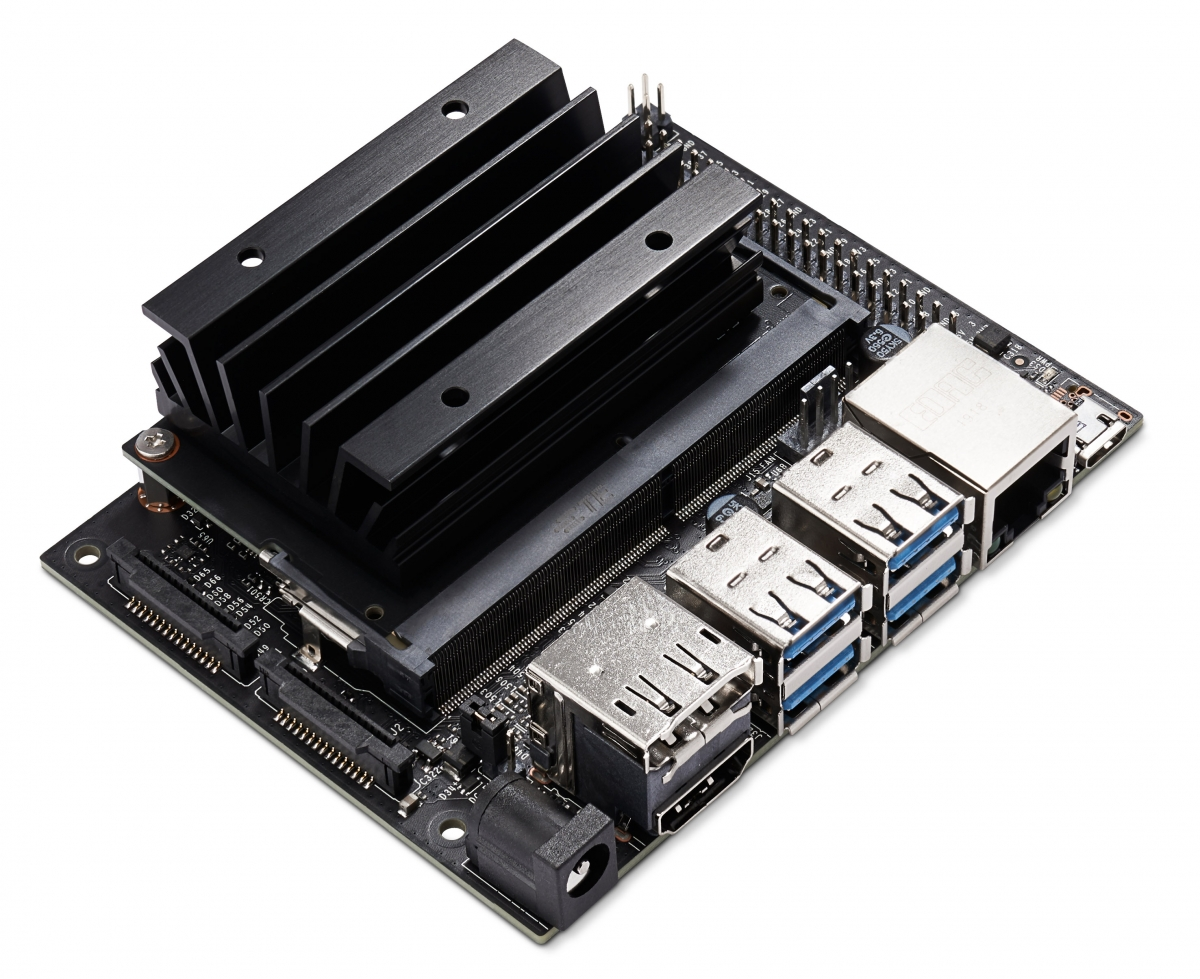
\includegraphics[scale=0.2]{fig/JetsonNano-DevKit_Front-Top_Right_trimmed.jpg}
    \caption{Jetson nano \cite{Jetson}}
\end{figure}

\subsection{Coral Edge TPU}
Google's Coral Edge Tensor Processing Unit (TPU) is a type of custom-built circuit known as an "application-specific integrated circuit" or ASIC. This TPU is specifically designed for deep learning inference, which involves making predictions from new data using a trained machine learning model. Similar to the GPU embedded in the Jetson Nano, this hardware is believed to execute object detection based on deep learning more rapidly than a CPU in a typical single-board computer. The Coral Edge TPU is a USB device, meaning it needs a computer to function.\\

Our interest in the Coral Edge was driven by its light weight and compact size. Coupled with a Raspberry Pi single-board computer, it would create a system that is cost-effective and light, ideal for our project requirements. We were keen to explore the performance potential of this hardware combination.\\

\begin{figure}[h]
    \centering
    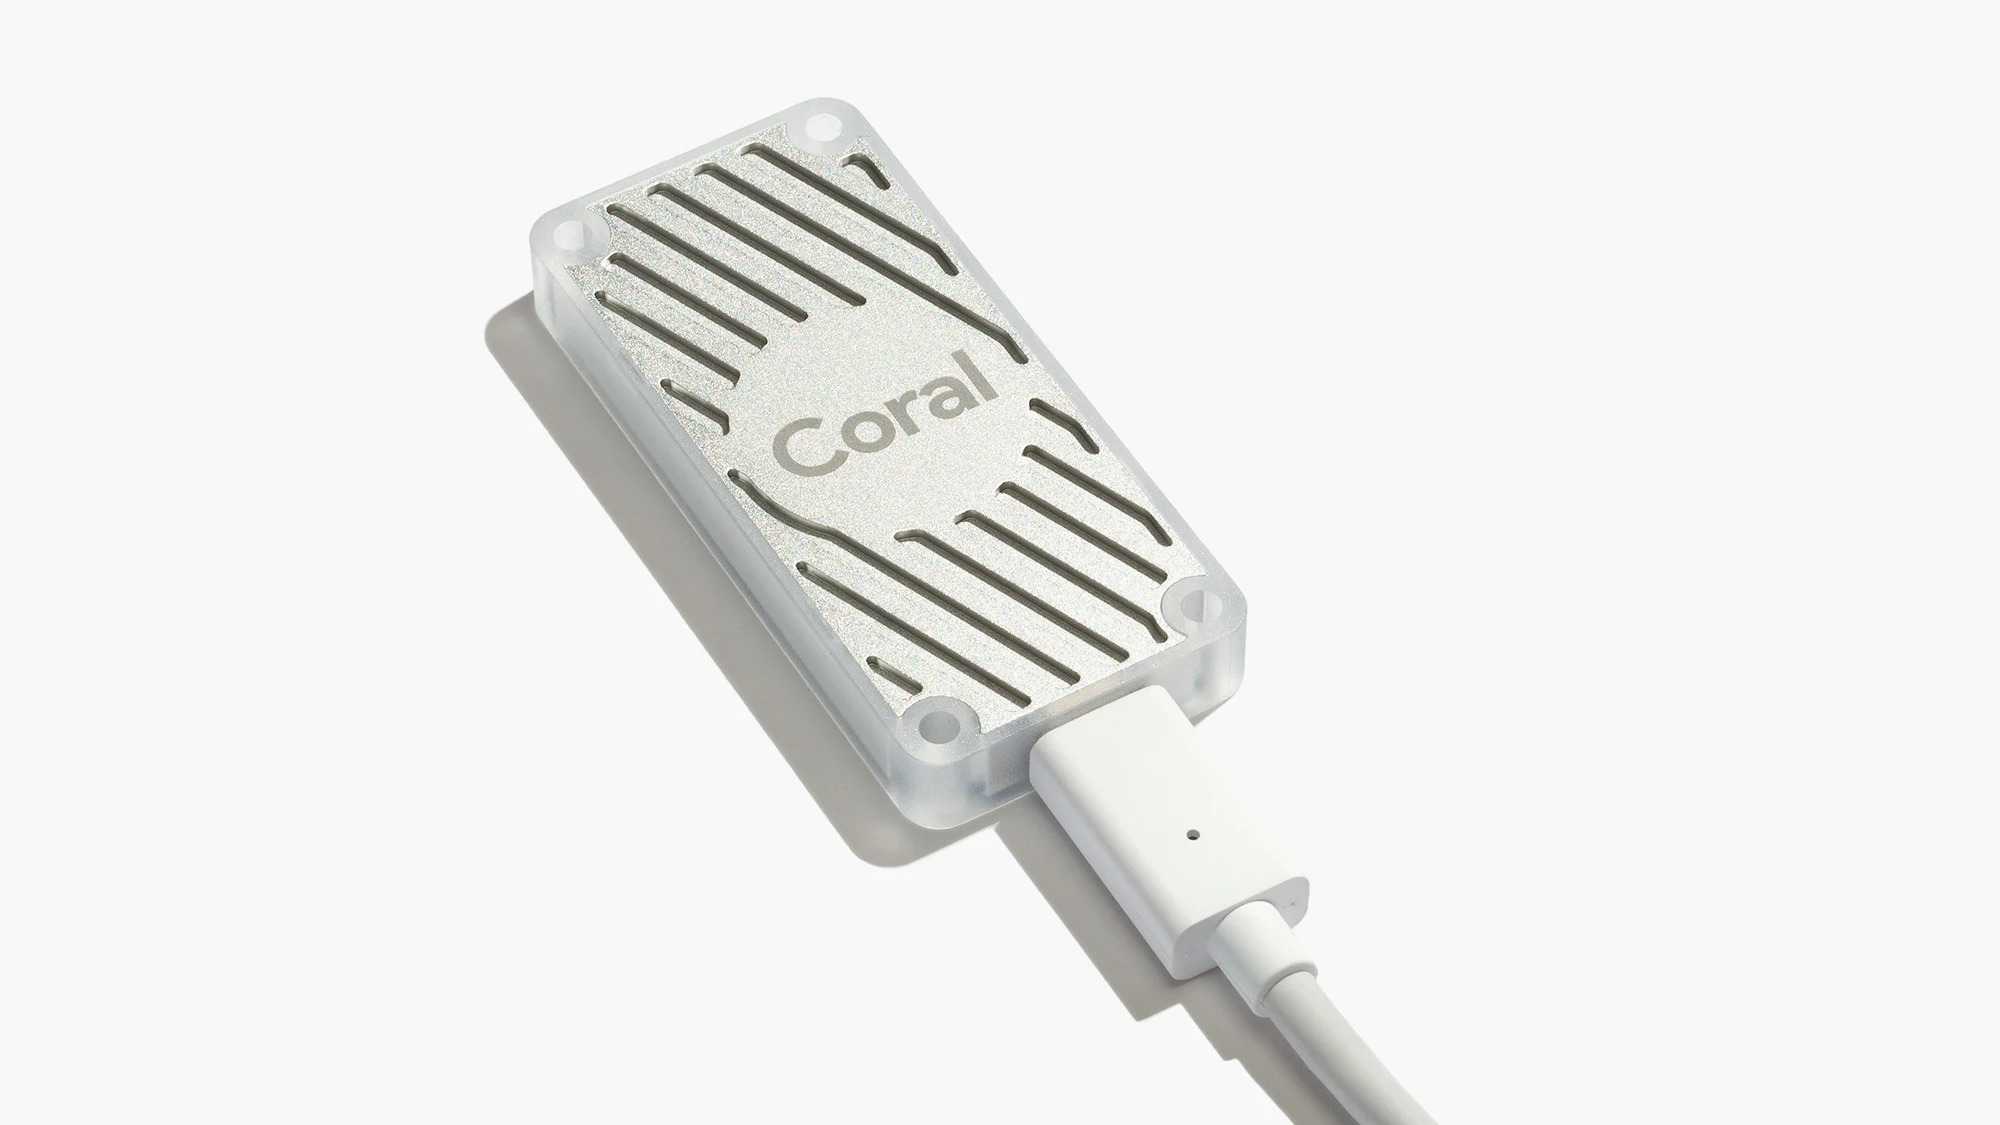
\includegraphics[scale=0.1]{fig/Coral TPU.jpg}
    \caption{Coral USB accelerator \cite{CoralTPU_bilde}}
\end{figure}


\subsection{Raspberry Pi 4B \& Zero 2}

The Raspberry Pi 4B and Raspberry Pi Zero 2 were chosen as integral components for the lightweight drone system due to their blend of power, flexibility, and cost-effectiveness.\\

The Raspberry Pi 4B's quad-core processor offers impressive computational power in a compact package, making it capable of handling complex tasks like navigation algorithms. On the other hand, while the Raspberry Pi Zero 2 is less powerful, it remains a competent device for managing lighter tasks within the system, making the two boards a complimentary pair.\\

An important consideration for drone applications is the weight and size of components. Both the Raspberry Pi 4B and Pi Zero 2 excel in this regard with their lightweight and compact form factors that do not compromise the flight time or maneuverability of the drone.\\

Cost-effectiveness is another compelling factor that makes these boards an attractive choice. They are significantly more affordable than other single-board computers of similar capabilities, fitting well within projects constrained by budget without sacrificing functionality.\\

Raspberry Pi's flexibility is also notable due to the broad range of available peripherals, such as cameras and sensors. These can be seamlessly integrated into the system, providing great versatility when constructing the drone setup. Additionally, the Raspberry Pi benefits from extensive software support and a large, active community. With the ability to run various Linux distributions, software development and troubleshooting become much easier tasks.\\

Finally, the Raspberry Pi offers scalability for future expansions or modifications. With numerous Raspberry Pi models available, it is feasible to scale the system up or down according to the changing requirements. For instance, upgrading to a more powerful Raspberry Pi model to accommodate increased computational demand or additional features can be done without substantially altering the system's architecture.\\

All these reasons underscore why the Raspberry Pi 4B and Raspberry Pi Zero 2 are optimal choices for a lightweight, efficient, and robust drone system.\\

\subsection{Pi Camera modules}

The Raspberry Pi Camera Module v2 and v3 were chosen as key components for our lightweight drone system due to their high-resolution capabilities, light weight, compatibility, and affordability. In addition to this, several group members already owned the version 2 of the camera, and this was available on the Jetson Nano.\\

The Raspberry Pi Camera Module v2 is equipped with an 8-megapixel sensor, capable of capturing high-resolution images and video, which is vital for effective image processing and object detection tasks. It provides impressive image quality, ensuring the data collected by the drone is clear and detailed.\\

On the other hand, the Raspberry Pi Camera Module v3 offers an even higher resolution with its 11.9-megapixel Sony IMX708 sensor. This module delivers crisp, high-quality images and better low-light performance, crucial for varied and unpredictable flight environments.\\

Both camera modules are exceptionally lightweight and compact, which is an essential aspect for drone-based applications. By using these camera modules, we avoid adding substantial weight to the drone, thereby maintaining optimal flight time and maneuverability.\\

In addition, both camera modules are fully compatible with the Raspberry Pi ecosystem, which assures seamless integration into our drone setup. The ability to directly connect these modules to the CSI camera port on Raspberry Pi boards enables efficient data transmission and simplifies the overall system design.\\

Lastly, similar to the Raspberry Pi boards, these camera modules are cost-effective. They offer high-quality imaging capabilities at a fraction of the cost of many other comparable camera modules. This affordability makes them an ideal choice for projects operating on tighter budgets.\\

In summary, the Raspberry Pi Camera Module v2 and v3 provide the perfect blend of performance, compatibility, and affordability for our drone system. They offer high-quality visual data, which is essential for tasks such as object detection and navigation.\cite{rpicam3specs}\cite{rpicam2specs}\cite{rpicamspecs}\\

%The Raspberry Pi Camera Module v2 was introduced in April 2016 to replace the original Camera Module. The v2 Camera Module is equipped with a Sony IMX219 8-megapixel sensor, which represents a significant upgrade from the 5-megapixel OmniVision OV5647 sensor found in the original camera. The Camera Module is capable of capturing high-definition video and still photographs. It is user-friendly for beginners, but also offers advanced features for users seeking to expand their knowledge. Online examples showcase the camera's versatility for time-lapse, slow-motion, and other video applications, while libraries provided with the camera facilitate the creation of special effects.\\

%Further details about the IMX219 and the Exmor R back-illuminated sensor architecture are available on Sony's website, underscoring that the camera's improved resolution represents a leap forward in image quality, color fidelity, and low-light performance. The Camera Module supports 1080p30, 720p60, and VGA90 video modes, in addition to still capture. It attaches via a 15cm ribbon cable to the Camera Serial Interface (CSI) port on the Raspberry Pi, and is compatible with all models of Raspberry Pi 1, 2, and 3. The camera can be accessed through the Multi-Media Abstraction Layer (MMAL) and Video for Linux (V4L) APIs, and numerous third-party libraries are available, such as the Picamera Python library. A "Getting Started with Picamera" resource is available for users seeking guidance on its use. The Camera Module is widely employed in home security applications, as well as in wildlife camera traps.\cite{rpicam2specs}\cite{rpicamspecs}\\

%\subsection{Pi Camera module v3}
%The Raspberry Pi Camera Module 3 is a compact camera designed by Raspberry Pi, equipped with a 12-megapixel sensor featuring high dynamic range (HDR) and phase detection autofocus. The camera is available in standard and wide-angle variants, both with or without an infrared cut filter.\\

%Capable of capturing full HD video and still photographs, the Camera Module 3 includes an HDR mode for up to 3 megapixels. Its operation is fully supported by the libcamera library, and its rapid autofocus feature makes it accessible to beginners while providing ample functionality for advanced users. The Camera Module 3 is compatible with all Raspberry Pi computers and features the same printed circuit board (PCB) size and mounting holes as its predecessor, the Camera Module 2. The only difference in dimension is the height, with the improved optics making the Camera Module 3 several millimetres taller than its predecessor. \\

\section{Operating System and System Software Decision Process}

In the pursuit of rigorous research and robust information, the significance of a controlled environment and reproducible results cannot be overstated. Absent these, the applicability and value of our findings risk being limited, particularly under rigorous scrutiny. A crucial component of establishing this controlled environment involves ensuring uniformity in our software across all configurations to the greatest feasible extent. This is to prevent the introduction of performance artifacts that could significantly impact performance, such as inconsistencies in software libraries or versions. In figure \ref{fig:operating_system_proposed} you can see how we envisioned our platform to function.\\

\begin{figure}[H]
    \centering
    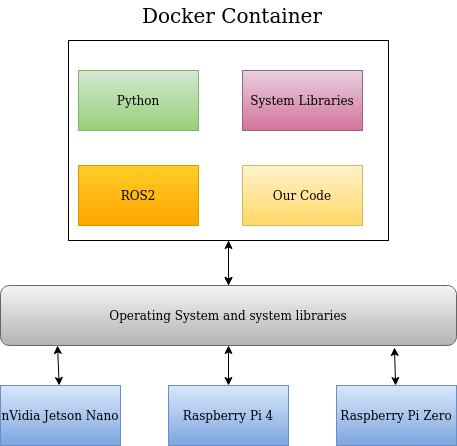
\includegraphics[scale=0.5]{fig/osdiag.png}
    \caption{Proposed Operating System Configuration}
    \label{fig:operating_system_proposed}
\end{figure}

In order to efficiently run the necessary software, we required a system configuration with robust hardware support. This system had to be compatible with a variety of Raspberry Pi hardware and the nVidia Jetson Nano. We decided to utilize the Python interpreted language for rapid prototyping. For the middleware and communication layer, we chose ROS2. \\

\textbf{ROS2 Introduction and Rationale}

Our first four proposals outlined in Section \ref{fig:architecture} each offer a certain degree of distribution. Distributing data processing across multiple hardware units necessitates machine-to-machine communication, a task for which the client specifically requested the use of ROS2. ROS2 is a comprehensive software suite designed for robotics, with its core feature being inter-process communication. By creating and building our software as ROS2 nodes, we can avoid dealing with networking complexities, as ROS2 abstracts them. In ROS2, nodes constitute a graph where edges represent topics. Nodes can publish and subscribe to these topics.\\

%Our first four initial proposals in \ref{fig:architecture} are all distributed to a degree. Distributing the data processing across multiple hardware units requires machine-to-machine communication. The client requested the use of ROS2 for this task. ROS2 is a software suite for robotics and its core feature is inter-process communication. By developing and building our software as ROS2 nodes we don’t have to deal with networking as this is abstracted away by ROS2. Nodes in ROS2 make up a graph where the edges represent topics. A node can publish and subscribe to topics.\\

\begin{figure}[H]
    \centering
    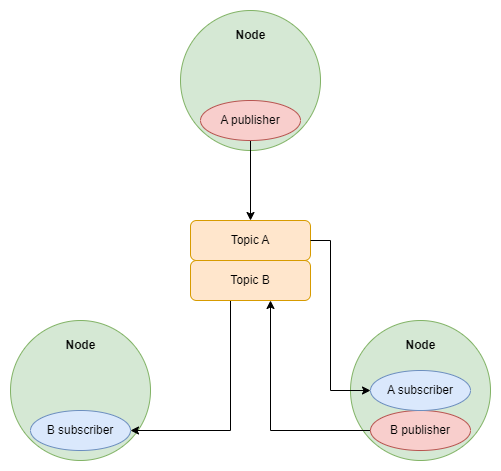
\includegraphics[scale=0.5]{a_martinbilder/ros_graph_example.png}
    \caption{Example ROS2 graph}
    \label{fig:ros_graph_example}
\end{figure}
Figure \ref{fig:ros_graph_example} presents a potential configuration of a ROS2 graph featuring three nodes. Beyond managing low-level communication between hardware units, integrating ROS2 contributes to high modularity, fostering the possibility for significant scalability. Upon reviewing our initial configurations, our client voiced interest in incorporating an additional single-board computer to further distribute the workload. This hardware expansion could also be implemented at subsequent stages without necessitating code rewrites. Essentially, nodes can be easily transferred from one hardware unit to another.\\

%Figure \ref{fig:ros_graph_example} illustrates how a ROS2 graph could look with three nodes. In addition to handling the low-level communication between hardware units, a ROS2 integration provides high modularity which creates a potential for high scalability. When proposed with our initial configurations, our client expressed their interest in adding an additional single board computer to further split up the workload. Adding hardware like this could also be done at later stages without rewriting any code. Nodes can simply be moved from one hardware unit to another.\\
\newpage

Our objective was to make an informed decision, ensuring we did not default to conventional software without considering potential alternatives that might offer performance benefits or simplified software deployment. Both the Raspberry Pi variants and the Jetson Nano are compatible with the Linux operating system. Linux, a free and open-source operating system, is available in several versions, commonly referred to as distributions or "distros". These distributions can greatly vary in terms of software availability and hardware support, contingent on the installed version. Consequently, we aimed to investigate the potential differences between these versions to determine which one best met our needs.

However, with over 600 distinct Linux distributions available, it was not feasible to evaluate all of them within our limited timeframe. To streamline our focus, we decided to sample the most commonly used distributions that also maintain an enterprise presence. Ultimately, we chose to evaluate Raspberry Pi OS, the version bundled with Raspberry Pi variants, along with Fedora Linux, openSUSE Linux, and Ubuntu.\cite{linuxcounter} \\ 

\newpage

After finalizing our decision, we turned our attention to designing our architecture, considering how the software would function on different hardware configurations and how we could ensure a uniform configuration across all systems. To this end, we explored the feasibility of running the software within what is commonly known as a container. A container is a compact, standalone, and executable software package that encompasses everything required to execute a piece of software, including the code, runtime, system tools, system libraries, and settings. Containers are isolated from each other and bundle their own software, libraries, and configuration files, communicating through well-defined channels. Implementing this technology would guarantee identical deployment configurations and could help mitigate any potential performance artifacts. The goal of this configuration was to encapsulate the necessary environment and libraries for ROS2 within these containers, as illustrated in Figure \ref{fig:dockerarch}.\\

\begin{figure}[H]
    \centering
    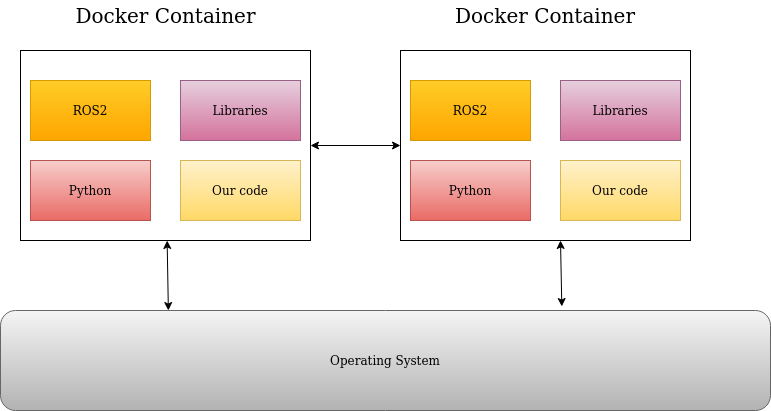
\includegraphics[scale=0.5]{fig/Docker Architecture.drawio.png}
    \caption{Docker architecture}
    \label{fig:dockerarch}
\end{figure}

Upon deciding which configurations to investigate, we initiated our examination by methodically installing the different distributions on physical hardware and assessing their functional capabilities and any shortcomings. As illustrated in Figure \ref{fig:osarch}, you can observe the different outcomes and ascertain which functions were successful and which were not. \\ 

\begin{figure}[H]
    \centering
    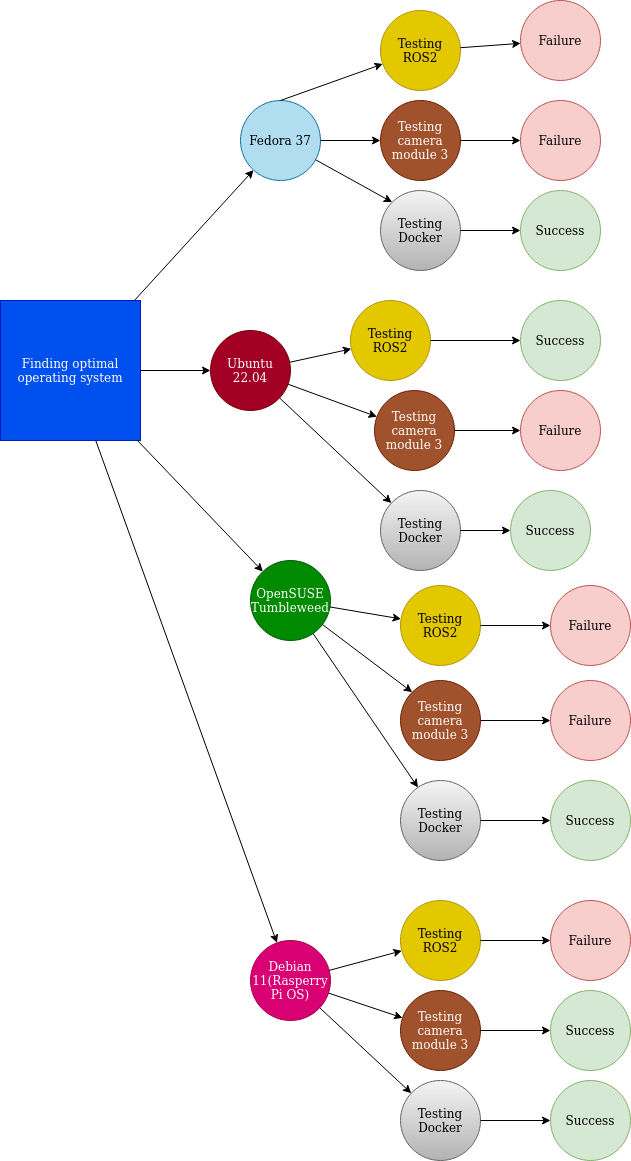
\includegraphics[scale=0.5]{fig/decision_os.png}
    \caption{Decision Process OS}
    \label{fig:osarch}
\end{figure}

\clearpage

As indicated in figure \ref{fig:osarch}, there were no systems that met all the requirements we had for our software platform, this caused a need to do further research in order to be able to decide which platform we would use going forward. \\

We further refined our choices to Ubuntu and Debian, as these platforms had only a single missing dependency. However, we needed to ascertain which option would offer the best outcomes relative to the efforts required to rectify each system.\\

\begin{figure}[H]
\centering
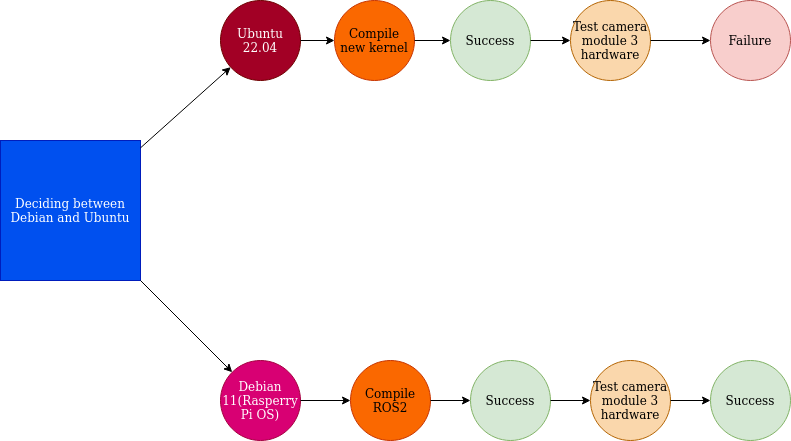
\includegraphics[scale=0.5]{fig/select_dist.png}
\caption{Decision Process Distribution}
\label{fig:distselect}
\end{figure}

Debian faced the disadvantage of having difficulties with the ROS2 operation, which entails a relatively complex and comprehensive build-system. The documentation can often be outdated due to the fast-paced advancement of the ROS2 project at the current stage. Conversely, Ubuntu's challenge lay in the lack of driver software for the Camera Module Version 3.\\

Given our limited experience with the ROS2 build system and the scant documentation on manual software building and installation, we decided to attempt installing the existing Debian driver in an Ubuntu environment. This would enable us to operate ROS2 with Camera Version 3.\\

\newpage

In the Linux operating system, drivers are typically formulated as modules and integrated with the operating system kernel. This kernel is the software component within an operating system that manages hardware resources. Within the Linux system, it is feasible to specifically compile this component for the running system, without interfering with the other system software components.\\

Our next step was to clone the git repository of the Raspberry Pi Foundation, given that the operating system bundled with these single-board computers (SBCs) supports that particular camera. Once completed, we managed to compile the Raspberry Pi OS kernel for our active version of Ubuntu.\\

After finalizing the installation and booting our new kernel, the hardware was detected, but there was no video output. At this juncture, we believed that we could get the hardware to function under Ubuntu, considering this as our best immediate course of action.\\

We proceeded with various tests under different configurations and compiled different versions of the Linux kernel, including an unmodified version directly from \url{https://kernel.org}. When none of these strategies produced the desired results, we were compelled to reassess our approach.\\

Our focus then transitioned towards an attempt at compiling ROS2 for Debian. We delved into the documentation to compile the software on our system. However, this task proved challenging, and we faced several hurdles while attempting to compile the software. As a temporary solution, we found someone who had compiled a Debian package on GitHub, albeit from an older build. We could not verify its applicability to our requirements, thus leaving us with necessary steps to continue deploying ROS2 while we concurrently operated an unsecured ROS2 installation, aiming to expedite development.\\

Following an extended period of continuous effort, we managed to compile ROS2 under a Debian system. This development allowed us access to Camera Module 3 and ROS2 on the same computer. The subsequent step involved deploying this to a Docker image, facilitating environment control and ensuring a consistent platform for our ROS2 source code.\\

However, an unfortunate consequence of compiling software is its substantial size growth. Post-building our Docker system, its size ballooned to 14GB, which was unwieldy for deployment and challenging to run on the Raspberry Pi Zero. Unfortunately, we were unable to rectify this issue in time for our project delivery. Although it does operate on the Raspberry Pi Zero, deployment is slow and can potentially create problems if the Zero exhausts memory while pulling the Docker image.\\

\subsection{Raspberry Pi 4 and Zero 2}
After reviewing our results from the selection process, we arrived at a proposed solution for our configurations based on the Raspberry Pi hardware and the Raspberry Pi OS. This solution mirrored the one depicted in figure \ref{fig:dockerarch}, thereby aligning closely with our initial research and concept.\\

\subsection{Jetson Nano System Software Configuration}

Upon finalizing the configuration for the Raspberry Pi, we shifted our focus to the Jetson Nano. Our initial plan was to have identical configurations across all hardware. However, the proprietary nature of Nvidia's hardware precluded the support of the Raspberry Pi OS.
This necessitated exploratory research on compatible software for the Jetson Nano, which would align closely with the Raspberry Pi configurations. We direct your attention to figure \ref{fig:jetsonnanodesc}, depicting the versions we attempted to install and set up on the hardware.\\

\begin{figure}[H]
    \centering
    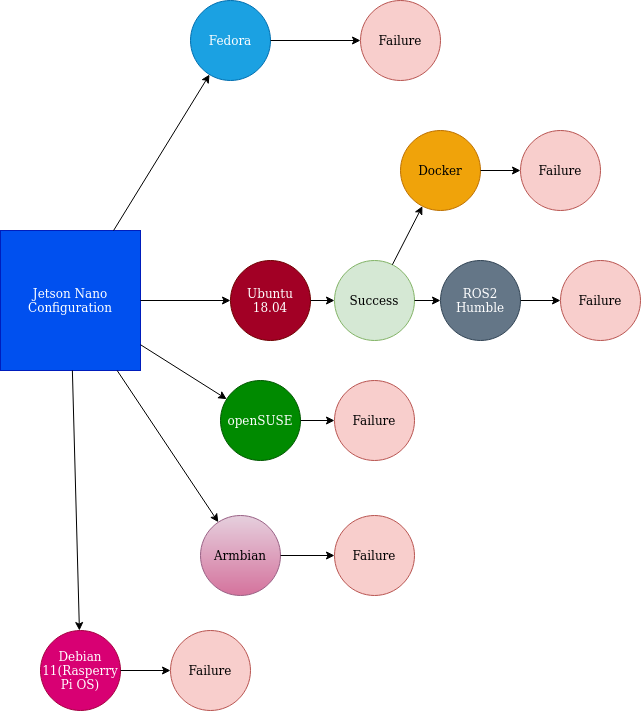
\includegraphics[scale=0.5]{fig/jetson_nano_os.png}
    \caption{Jetson Nano Decision Map}
    \label{fig:jetsonnanodesc}
\end{figure}

Following a rigorous testing phase where we attempted to run several different distributions on the Nano, we concluded that this approach was not an efficient use of our time. We chose instead to focus on executing the docker architecture on the bundled Ubuntu version running on the Jetson Nano. The supported version was released in April 2018. Despite its age, we believed that since Docker was available for it, we could adjust our container setup to secure a controlled environment to the extent possible.\\

\textbf{Docker Environment Jetson Nano}

When considering Docker on the Nano, we decided to implement the same configuration we had functioning on the other systems. However, adapting this to the hardware and software on the Nano proved challenging. Nvidia distributes the necessary software for the Nano in packages referred to as "Jetpacks". These packages are designed for use on specific versions of Linux that they ship with Jetson Nano; our version of the Jetson Nano was supported on Ubuntu 18.04, a five-year-old distribution. This presented challenges due to the rapid pace of change in many of the frameworks and Python libraries we wanted to use. Similar factors were also present in terms of features and performance improvements in the operating system itself.\\

Creating a Docker environment where we pass the GPU and every required library into the container in a functional manner proved to be a complex task. It demanded more expertise and time than we could provide during our project. Ultimately, the challenges posed by the Jetson Nano forced us to reconsider our architectural idea.\\

The final result for our Jetson Nano was that we utilized the system software bundled with the hardware, specifically Ubuntu 18.04. Owing to issues with Docker, we ran the software on the bare metal, as illustrated in figure \ref{fig:jetsonnanoros}. Moreover, unlike the Raspberry Pi configurations running ROS2 Humble, the Nano operates ROS2 Dashing. Despite these differences, the ROS2 architecture remains identical to the other configurations.\\

\begin{figure}[H]
    \centering
    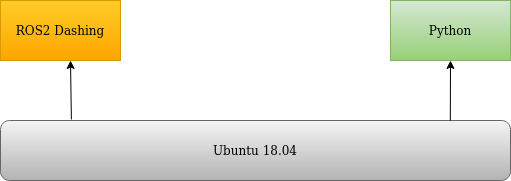
\includegraphics[scale=0.35]{fig/jetsonros.drawio.png}
    \caption{End Result Jetson Nano Architecture}
    \label{fig:jetsonnanoros}
\end{figure}
\newpage

\subsection{32-bit vs. 64-bit}
As Raspberry Pi OS 64-bit beats 32-bit in almost every metric regarding computation time \cite{32-bit_vs_64-bit} we decided to omit 32-bit based operating systems as a contender from this project.

\section{Proposed architectures}
\subsection{Initial Proposal}

Before we could start implementing our specific designs we needed to get the go-ahead from our client. We made a design sketch with five different configurations and presented these in order to reach an agreement on which areas we should focus on.

\begin{figure}[!h]
    \centering
    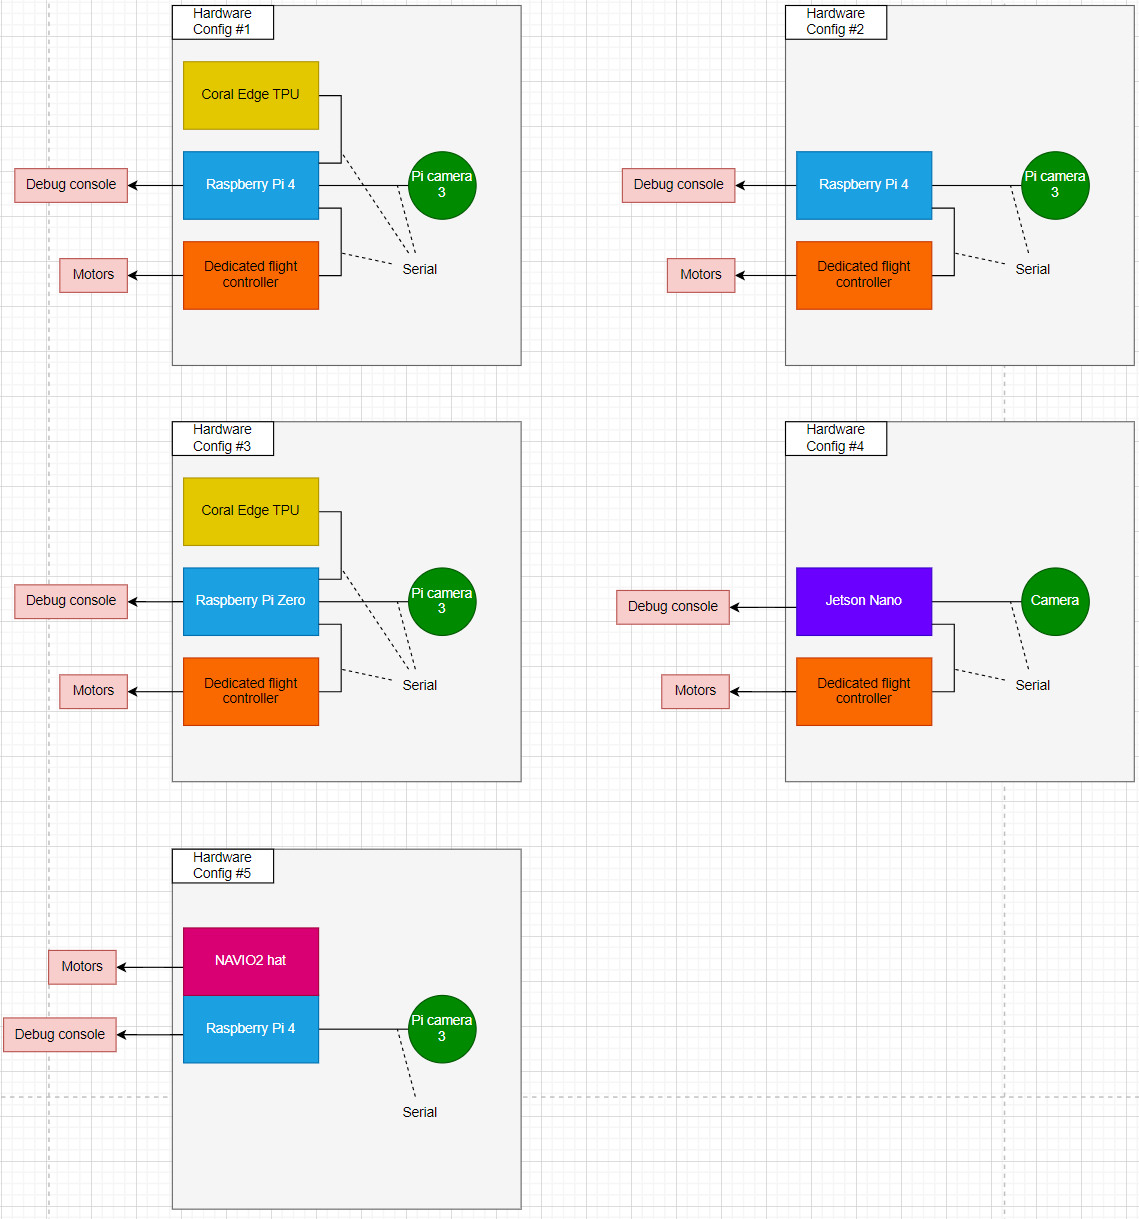
\includegraphics[scale=0.35]{fig/arkitektur.png}
    \caption{Initial architecture design}
    \label{fig:architecture}
\end{figure}
\newpage

From the figure \ref{fig:architecture} in this figure, you can see the five proposals which we presented to the client. These proposals were based on a variety of hardware configurations we had briefly discussed during meetings and the ones that we thought were the most likely to achieve our client's goals and deliver results that would show that this idea was viable. \\

\subsection{Second proposal}


\begin{figure}[H]
    \centering
    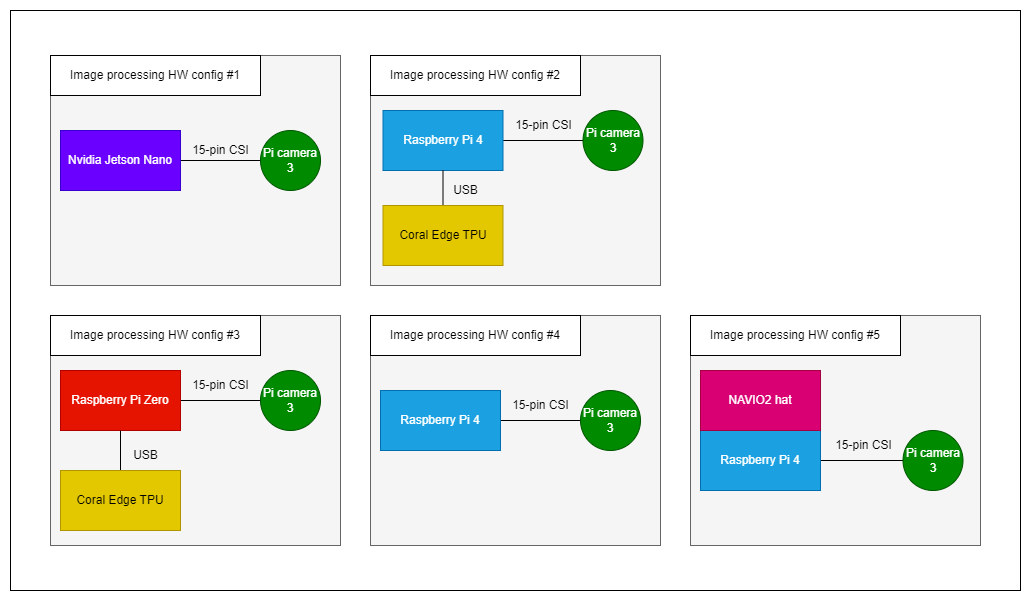
\includegraphics[scale=0.5]{a_martinbilder/hw_proposal2.drawio.png}
    \caption{Image processing modules}
    \label{fig:image_processing_prop2}
\end{figure}

\begin{figure}[H]
    \centering
    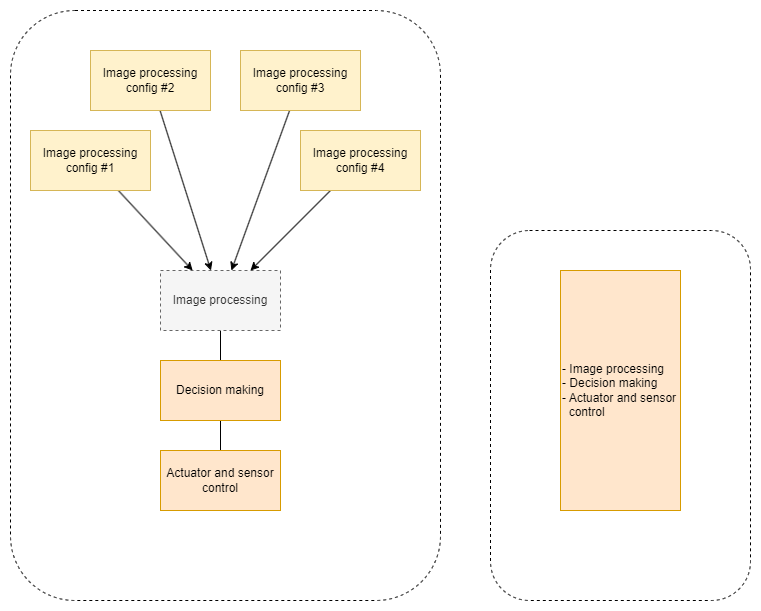
\includegraphics[scale=0.5]{fig/DistributedVsCentralized.png}
    \caption{Four distributed and one centralized architecture}
    \label{fig:distributed_vs_centralized}
\end{figure}

Figures \ref{fig:image_processing_prop2} and \ref{fig:distributed_vs_centralized} describe the second iteration of our hardware configuration designs. Our image processing hardware is now drawn as interchangeable modules, which plug into the rest of the drone. The “Decision making” module in \ref{fig:distributed_vs_centralized} represents a new single board computer, and the “Actuator and sensor control” module is the flight controller.
After further discussing our proposals with the client we agreed to drop configuration 5 due to time constraints. Discarding the centralized configuration gave us more time to explore image processing software, which at this point seemed to be the most time-consuming task ahead.\\

\subsection{Accepted architectures}
\label{sub:accepted_architectures}

Figure \ref{fig:accepted_hw_architectures} illustrates the final hardware architectures which were accepted by the client.

\begin{figure}[H]
    \centering
    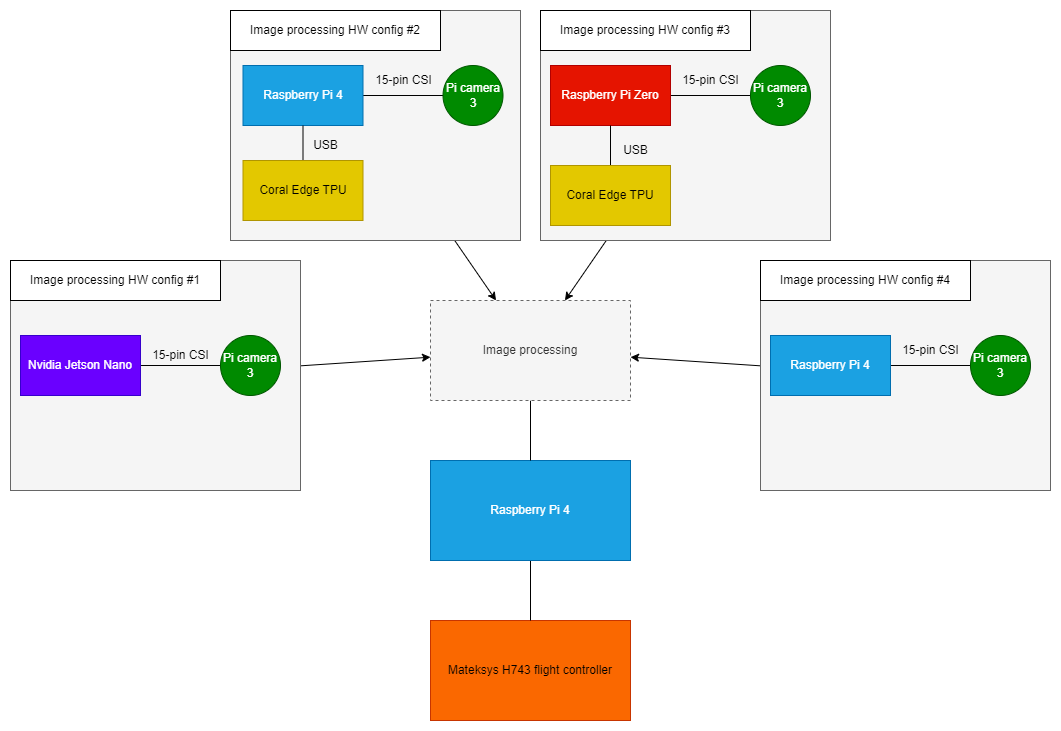
\includegraphics[scale=0.45]{a_martinbilder/accepted_hw_architecture.png}
    \caption{Hardware architectures accepted by client}
    \label{fig:accepted_hw_architectures}
\end{figure}


At this stage we had designed a high-level software architecture which shows our planned ROS2 nodes and how they should interface with each other. The architecture shown in figure \ref{fig:initial_software_architecture} is common for all our configurations. We decided that all 4 image processing modules should output the estimated distance to a detected object, and the detected object’s X and Y coordinates within the image frame. As a demonstration of a use case which needs the distance and position data, we designed the software architecture with “object following” in mind. For this use case the “Follow algorithm” node in figure \ref{fig:initial_software_architecture} would be a regulator which decides how the UAV should move to follow the detected object.

\begin{figure}[H]
    \centering
    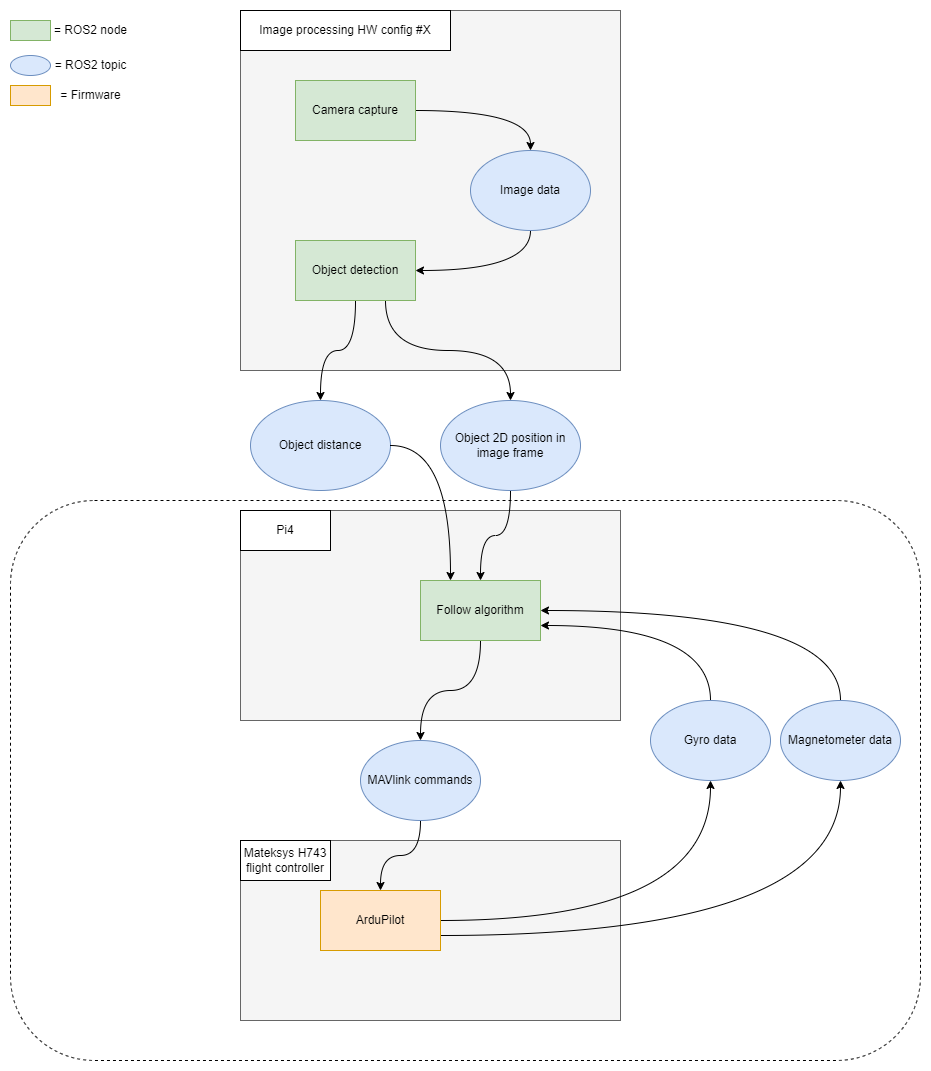
\includegraphics[scale=0.5]{a_martinbilder/initial_software_arch.drawio.png}
    \caption{Initial software architecture design}
    \label{fig:initial_software_architecture}
\end{figure}



\section{Object detection software}

One of the object detection systems we wanted to use was YOLO.\\

The YOLO (You Only Look Once) framework, developed by Joseph Redmon, revolutionized the field of object detection by providing a real-time object detection system. Contrary to traditional two-step object detection methods, where one step is dedicated to proposing regions where objects might exist and the second to classifying those regions, YOLO performs both tasks in one step. This makes it significantly faster and more efficient, which is particularly beneficial for applications that require real-time detection.\cite{YOLO}

The architecture of YOLO involves dividing the input image into a grid. Each grid cell predicts a certain number of bounding boxes and class probabilities. During the detection phase, bounding boxes with class probabilities below a certain threshold are discarded.

YOLO has gone through several iterations to improve its performance, in this study we have looked at YOLOv5 (released June 25th, 2020) \cite{YOLOv5}, and the latest YOLOv8 (released January 10th, 2023)\cite{YOLOv8}, both released by Ultralytics.

Given the novelty of YOLOv8, there was a lack of documentation regarding its operation on a Jetson Nano. All the available information concerning YOLO's operation on a Jetson Nano pertained to YOLOv5. Therefore, after meticulous comparison and deliberation, the decision was made to transition to the earlier iteration, YOLOv5.

Despite the commendable efforts of Ultralytics to simplify the application of YOLO, mastering the process of training on our own dataset, and effectively utilizing the diverse set of tools that accompany the framework, demanded a considerable investment of time. This learning curve demonstrates the complexity inherent in working with such advanced object detection systems. Readers are referred to the \ref{appendix:Yolo Training Tutorial} appendix for a concise guide on how to train models with custom data. Additional information and comprehensive documentation can be found on the Ultralytics website.

\subsubsection{Dataset}

In this study we decided on a common dataset for all the object detection models to be trained on. The dataset is divided into three distinct subsets - training, validation, and testing sets - each consisting of 110, 32, and 30 images respectively. The training set is used during the learning process, the model is then validated on the validation set at the end of each epoch. The test set is a dataset never seen before by the model and is used to do a final validation of the model.
Since we wanted to have a comparison between object detection and blob detection, we decided on a green tennis ball being the target for our models as this is easier to capture with blob detection.  


\section{Distance Measurement}

After wishes from our client, we've included the capability to calculate the distance to a detected object in our project. This is especially useful when considering the drone's relative position to the object and is particularly relevant for use cases such as landing. Understanding this distance becomes a key factor in ensuring precise and controlled landing maneuvers. \\

Due to the fact that we are using one singular camera, there is a problem getting the proper depth. The method we chose to use involves the idea of similar triangles to calculate the distance between a camera and an object. This method is based on the principle that the ratio of the object's actual width to its distance from the camera matches the ratio of the object's perceived width in the captured image (in pixels) to the camera's focal length. \cite{distanceobject}

To illustrate this concept mathematically, we introduce two similar triangles:

\begin{itemize}
    \item The first triangle (Triangle A) is constructed with the vertices being the camera, the object, and a selected point on the camera's image plane.
    \item The second triangle (Triangle B) includes the camera, the image of the object as perceived by the camera, and the identical point on the image plane as used in Triangle A.
\end{itemize}

In this scenario, the parameters for the two triangles are defined as follows:

\begin{itemize}
    \item In Triangle A, the 'height' is the distance to the object (D) and the 'base' is the actual width of the object (W).
    \item In Triangle B, the 'height' represents the camera's focal length (F), and the 'base' signifies the apparent width of the object in the image (P, in pixels).
\end{itemize}

Since the two triangles are similar, the ratios of the corresponding sides are equal, resulting in the equation:

\begin{equation}
\frac{D}{W} = \frac{F}{P}
\end{equation}

Using this equation, we can derive any one of the variables given the other three. For instance, the focal length of the camera (F) can be calculated by rearranging the equation to:

\begin{equation}
F = \frac{P \times D}{W}
\end{equation}

Furthermore, if the object's position shifts, altering the apparent width in the captured image (P'), the same equation can be adapted to compute the new distance (D'):

\begin{equation}
D' = \frac{W \times F}{P'}
\end{equation}



\section{Proposed Operating System and System Configuration}

After a comprehensive evaluation of operating systems suitable for various hardware configurations, we concluded that the Raspberry Pi configurations would utilize the system software provided with the devices. This decision was informed by the superior hardware support and the system's ability to effectively run ROS2 as required.\\

Contrarily, the situation with the Jetson Nano was distinct. Given the limited time for an in-depth exploration of the software construction on this platform, we decided to adhere to the configuration supported by nVidia. The final proposed system can be seen in Figure \ref{fig:sysconf}.

\begin{figure}[H]
    \centering
    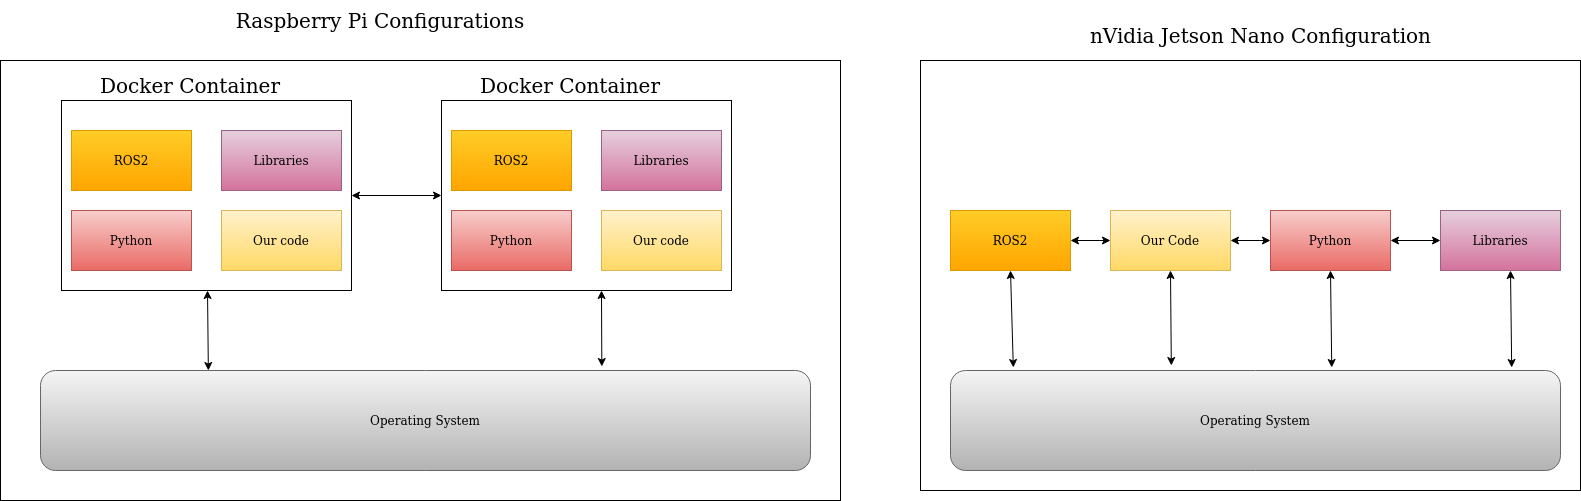
\includegraphics[scale=0.30]{fig/completeconfig.drawio.png}
    \caption{Finished Overview System Configuration}
    \label{fig:sysconf}
\end{figure}

\newpage

\section{Image processing modules}
In this chapter, we delve into the vital aspect of image processing configuration, a journey that has proven both challenging and enlightening. Our exploration began with an understanding of the integral role image processing plays in our project. As a technique that involves transforming or altering images using mathematical operations, image processing serves as a conduit that translates raw, visual data into a format that our systems can understand and utilize effectively.

Throughout this chapter, we discuss the myriad complexities involved in selecting, tuning, and applying appropriate image processing techniques and configurations. We recount our decision-making process, the technical considerations, the trial-and-error iterations, and the fortuitous insights that informed our eventual choices.

We acknowledge that the pathway toward effective image processing configuration is neither linear nor universally applicable. The optimal solutions often depend heavily on the specific contexts, goals, and constraints of the project at hand. However, we believe that by sharing our journey – our successes, our hurdles, and the lessons we learned along the way – we can provide valuable insights that may guide similar endeavors in the future.

Through this reflection, we aim to illuminate the depth and breadth of thought that underlies the seemingly mundane topic of image processing configuration, reinforcing its critical role in the success of our project and many others in the field. By the end of this chapter, readers will not only understand our journey toward an effective image processing configuration but also appreciate the intellectual richness that this journey entails.
\newpage

\subsection{Configuration 1, Jetson Nano}
This section aims to clarify the steps we followed to make object detection work on a Jetson Nano, incorporating details of unsuccessful attempts as well.

\begin{figure}[!h]
    \centering
    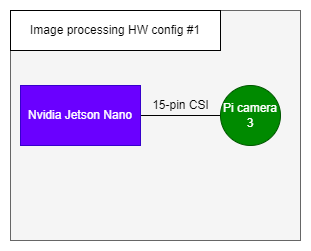
\includegraphics[scale=0.5]{fig/config1_hw.png}
    \caption{Hardware architecture, config 1}
    \label{fig:config1_hw}
\end{figure}


\subsubsection{Initial setup}

The NVIDIA Jetson Nano platform employs a software development kit (SDK) image known as JetPack, specifically version 4.6.1, which is the newest compatible version for the Jetson Nano device. JetPack 4.6.1 is built upon Ubuntu 18.04 (Bionic Beaver) and utilizes Python 3.6.9. The image is preconfigured with several essential developer tools, including TensorRT, cuDNN, and CUDA.\\

To flash the image onto the Jetson Nano, one can either use a terminal or the NVIDIA SDK Manager, which can be accessed at \cite{Jetson_sdk_manager}. It is strongly recommended to employ the NVIDIA SDK Manager for this task, as it significantly simplifies the installation process for the image and any additional SDKs. However, this method necessitates that the computer used for flashing possesses the same operating system as the target image. In the present case, the computer required reformatting to Ubuntu 18.04 to ensure compatibility.\\



Alternatively, the SD card can be directly flashed using the terminal. The necessary image can be obtained from the NVIDIA developer site \cite{Jetpack_461}. Subsequent instructions specific to your operating system can be found at \cite{Jetpack_461_write_to_sd}.\\

Following this, the NVIDIA SDK Manager can be used to install all additional SDKs via Secure Shell (SSH). This approach upholds the user-friendliness and efficient process inherent to the SDK Manager.

\subsubsection{Software overview}
Camera interface: Gstreamer and openCV\\
Object detector type: Deep neural network\\
Machine learning framework: Trained with Pytorch, TensorRT for inference\\
Model type: FP32 TensorRT model (.engine)\\
Model 1: 640x640x3 (Yolov5n)\\
Model output: Bounding boxes, prediction scores, class names, number of predictions\\
Model size: 7MB

\subsubsection{Config1 journey}


The process of getting infernece to run on the Jetson Nano platform has been a complex undertaking, with our efforts encompassing three distinct methodologies and two different models: MobileNet-SSD and YOLO. Each subsequent three subsection will delineate the specifics of these approaches. All methodologies employs TensorRT optimization to facilitate efficient execution on the NVIDIA hardware. The final method is the one currently in operation. see figure \ref{fig:storyline} for a visual representation of the journey.

\begin{figure}[H]
    \centering
    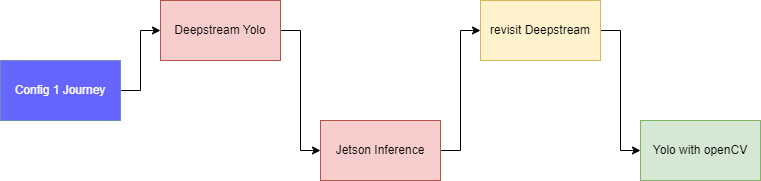
\includegraphics[scale=0.5]{evenbilder/storyline.drawio.png}
    \caption{Visual representation of the journey}
    \label{fig:storyline}
\end{figure}

\subsubsection{Yolo with Deepstream}
The process of deploying YOLOv5 on the Jetson Nano platform proved to be more complex compared to the implementation of MobileNet-SSD. The YOLOv5 documentation provides a dedicated page for its application on a Jetson Nano using a Software Development Kit (SDK) from Nvidia named Deepstream. However, the tutorial \cite{yolo_on_jetson}, last updated 18 November 2022) is not as straightforward as it might appear. For the purpose of this study, the deployment of YOLOv5 on the Jetson Nano was accomplished through two distinct approaches, both of which will be thoroughly explored in the following sections.


The initial step requires the use of a PC running Ubuntu 18.04 to operate the Nvidia SDK Manager in conjunction with the Jetson Nano. Following this, the installation of several additional packages, one of which is Deepstream, is necessary. This part of the procedure is fairly linear and should already be done with the initial setup of the Jetson.

The challenge arises when attempting to install dependencies for YOLO. Since YOLOv5 necessitates Python 3.7, while the Jetson Nano only supports Python 3.6.9, after cloning the repository, all entries in the requirements.txt file were commented out. Subsequent to numerous trials and errors, the tested system runs the following versions.

\begin{table}[H]
\centering
\begin{tabular}
{ |c|c| } 
\hline
Python package & Version number \\
\hline
gitpython & 3.1.20\\
\hline
matplotlib & 3.3.4 \\
\hline
numpy & 1.19.5 \\
\hline
opencv-python & 4.1.1\\
\hline
Pillow & 7.1.2\\
\hline
psutil & \\
\hline
PyYAML & 6.0\\
\hline
requests & 2.18.4\\
\hline
scipy & 1.5.4\\
\hline
thop & 0.1.1\\
\hline
tqdm & 4.64.1\\
\hline
seaborn & 0.11.0\\
\hline
setuptools & 59.6.0\\
\hline
\end{tabular}
\caption{pip packages used for deepstream}
\label{tab:yolo_requirements}
\end{table}
%gitpython>=3.1.20\\
%matplotlib>=3.3.4\\
%numpy>=1.19.5\\
%opencv-python>=4.1.1\\
%Pillow>=7.1.2\\
%psutil\\
%PyYAML>=6.0\\
%requests>=2.18.4\\
%scipy>=1.5.4\\
%thop>=0.1.1\\
%tqdm>=4.64.1\\
%seaborn>=0.11.0\\
%setuptools>=59.6.0\\


Continuing from this point, the subsequent steps as outlined on the GitHub repository should be followed until the DeepStream Configuration for YOLOv5 "Step 4. Generate the cfg and wts files". This can be accomplished with the following Python3 commands:

python3 gen\_wts\_yoloV5.py -w yolov5s.pt\\
python3 gen\_wts\_yoloV5.py -w custom.pt\\

Here, the user has the flexibility to either convert the pretrained yolov5s model or replace it with any model that has been subjected to transfer learning, as demonstrated above.

After completing the remaining steps, the user should be able to run inference on the included video. Additionally, to run inference on a Camera Serial Interface (CSI) camera, as employed in this study, the user must modify the source0 parameter in the deepstream\_app\_config.txt file as follows:



\begin{figure}[H]
    \centering
    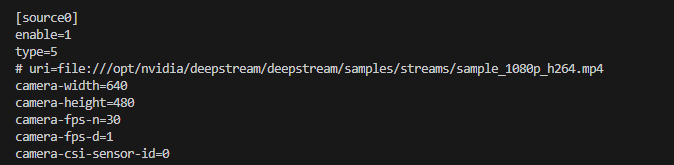
\includegraphics[scale=1]
    {evenbilder/yolo_deepstream_config.png}
    \caption{Deepstream app config file, source0}
    \label{yolo_deepstream_config}
\end{figure}

DeepStream offers built-in support for CSI cameras, with type=5 indicating the usage of a CSI camera. The camera's width and height can be adjusted according to the user's needs. It should be noted, however, that the model is optimized for an input resolution of 640x640 pixels, so providing an input close to this resolution would potentially enhance performance.\\

It is also important to modify the config-file under primary-gie, set this to config\_infer\_primary\_yoloV5.txt

To use a custom model, the configuration file must be modified in line with the particular version of YOLO in use, hence necessitating amendments to the 'config\_infer\_primary\_yoloV5.txt' file. The modifications include changes to the following parameters:

\begin{figure}[H]
    \centering
    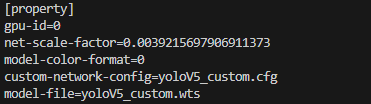
\includegraphics[scale=1]{evenbilder/yolo_deepstream__custom_model.png}
    \caption{config\_infer\_primary\_YoloV5.txt, custom model}
    \label{config_infer_primary}
\end{figure}

In this context, the weight (wts) and configuration (cfg) files have been renamed as 'yoloV5\_custom.cfg' and 'yoloV5\_custom.wts', respectively, indicating their customized nature and their association with the YOLOv5 model.
Now to run inference, simply use the command:\\
\\
deepstream-app -c deepstream\_app\_config.txt\\

As indicated on the Ultralytics webpage \cite{yolo_on_jetson}, the potential to achieve a rate of 30 frames per second (fps) exists when deploying a Jetson Xavier NX with FP32 and the YOLOv5s model. In contrast, the Jetson Nano, possessing lesser hardware capabilities than the Xavier, managed to reach a rate of 10 FPS with the YOLOv5n (Nano) model.

However, a substantial obstacle presented itself in the form of a 400 ms latency on the inference stream. Even with thorough system resource monitoring and various attempted solutions, the latency issue could not be mitigated. The implications of this problem suggested that the procedure overtaxed the Jetson Nano's hardware, thereby making it an unsuitable choice for applications like drone operations, which require instantaneous detection capabilities.

The Deepstream approach, despite its challenges, displayed a degree of adaptability. Specifically, it allowed a broad range of easy customizability via accessible configuration files.
\newpage



\subsubsection{Mobilenet-SSD}
Jetson Inference \cite{Jetson_inference}, a GitHub repository developed by Dustin Franklin from Nvidia, provides a well-documented tutorial complete with video walkthroughs, which is particularly beneficial for beginners in the field of computer vision working on the Jetson device. The process of getting this up and running is as simple as cloning the repo and then running the docker that is included. 

The pre-trained model demonstrated satisfactory performance at shorter distances but struggled with object detection when the objects were small or located at greater distances. To address this, transfer learning was applied to the model using our dataset, both on the Jetson device and on a separate computer equipped with a dedicated GPU. Despite training the model for over 1000 epochs, the inference failed to detect the object.

A survey of online forums confirmed that the model encountered difficulties with small objects. An attempt was made to upgrade the model to accommodate an input resolution of 512x512 instead of the standard 300x300. This was tried, and while this modification slightly improved the model's performance, it did not reach the level of the YOLO model trained earlier in the study. As a result, a decision was made to revisit YOLO.

\subsubsection{Yolo with openCV}

Since DeepStream did not yield satisfactory results, we searched for an alternative solution. During this exploration, we discovered newly created repository from Mailrocketsystems \url{https://github.com/mailrocketsystems/JetsonYolov5}. The repository applies TensorRT and OpenCV for inference. The configuration process is user-friendly, requiring merely adherence to the instructions provided in the repository's ReadMe file on GitHub.

The extraction of the right metadata from the model necessitates some modifications to the yoloDET script. Please refer to Figures \ref{fig:inference_before} and \ref{fig:inference_after} for the implemented changes.



\begin{figure}[H]
    \centering
    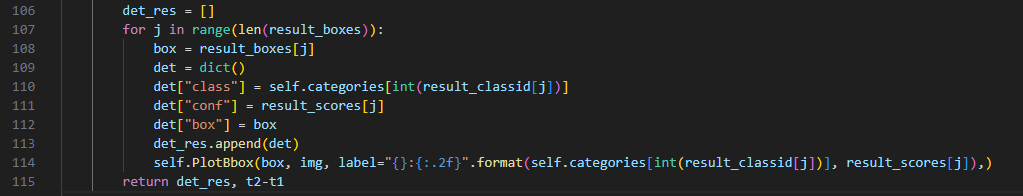
\includegraphics[scale=0.5]{evenbilder/yolo opencv/inference-before.png}
    \caption{YoloDET before}
    \label{fig:inference_before}
\end{figure}

\begin{figure}[H]
    \centering
    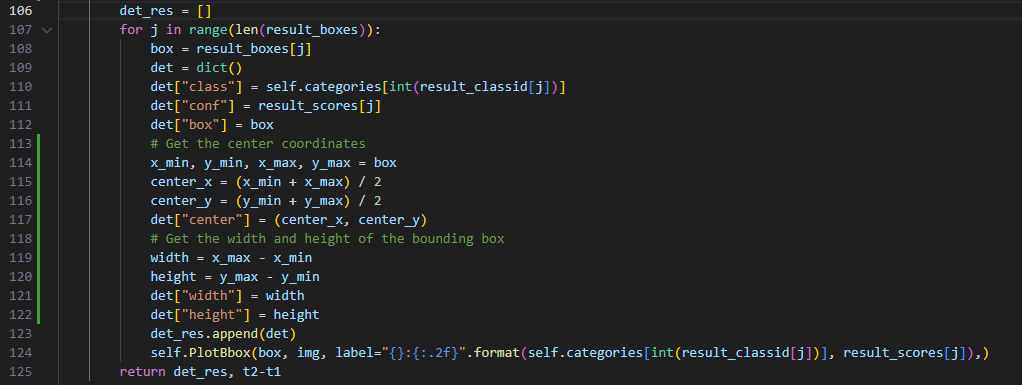
\includegraphics[scale=0.5]{evenbilder/yolo opencv/inference-after.png}
    \caption{YoloDET after}
    \label{fig:inference_after}
\end{figure}

Now we can simply edit the app.py script to use our model, and extract the metadata we just added in yoloDET. See figures \ref{fig:selecting_our_model}, \ref{fig:metadata_orginal}, \ref{fig:metadata_modified}\\

\begin{figure}[H]
    \centering
    
\includegraphics[scale=0.5]{evenbilder/yolo opencv/custommodel.png}
    \caption{Selecting our model}
    \label{fig:selecting_our_model}
\end{figure}

\begin{figure}[H]
    \centering
    
\includegraphics[scale=0.5]{evenbilder/yolo opencv/app1.png}
    \caption{extracting metadata original}
    \label{fig:metadata_orginal}
\end{figure}

\begin{figure}[H]
    \centering
    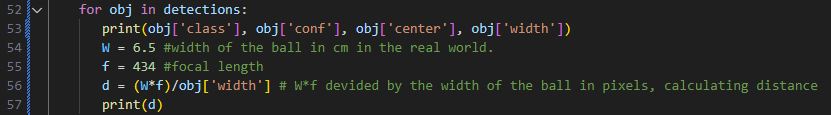
\includegraphics[scale=0.5]{evenbilder/yolo opencv/app2.png}
    \caption{extracting metadata modified}
    \label{fig:metadata_modified}
\end{figure}

The repository enabled us to perform inference in real-time with close no none latecy, which was particularly helpful in demonstrating the capabilities of the hardware within config1. 


\subsubsection{Reflections}


While the Jetson Nano boasts comparatively robust hardware, it is beginning to show signs of obsolescence, largely due to its reliance on an older version of the Jetpack SDK, which in turn is based on outdated versions of Ubuntu and Python. There have been considerable developments since Ubuntu 18.04 and Python 3.6. Nonetheless, we maintain that the Jetson Nano presents a compelling option for hobbyists seeking to delve into the realm of AI and explore its capabilities. For more advanced development pursuits, we would recommend a more contemporary model, such as the Jetson Orin Nano. This newer hardware is accompanied by support for the latest release of the Jetpack SDK, which is based on Ubuntu 20.04, and generally offers better compatibility with recent software.


The Jetson Nano was received quite late into the project, leaving us with approximately one month to set it up and get it working. With more time, and a deeper understanding of machine learning and ai, the results might have been different.


\newpage

\subsection{Configuration 2, Pi 4 w/ Coral Edge TPU}

\begin{figure}[h]
    \centering
    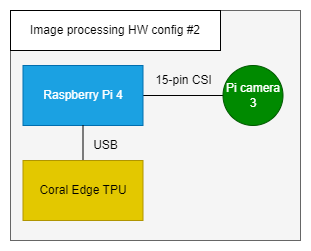
\includegraphics[scale=0.5]{fig/config2_hw.png}
    \caption{Hardware architecture, config 2}
    \label{fig:config2_hw}
\end{figure}


\subsubsection{Software overview}

\textbf{Camera interface:} picamera2 python library\\
\textbf{Object detector type:} Deep neural network\\
\textbf{Machine learning framework:} Tensorflow Lite\\
\textbf{Model type:} Tensorflow Lite model (.tflite) compiled for Coral Edge TPU\\
\textbf{Model 1 input:} 320x320x3 array (EfficientDet-lite0)\\
\textbf{Model 1 size:} 5.57MB (EfficientDet-lite0)\\
\textbf{Model 2 input:} 384x384x3 array (EfficientDet-lite1)\\
\textbf{Model 2 size:} 7.57MB (EfficientDet-lite1)\\
\textbf{Model outputs:} Bounding boxes, prediction scores, class names, number of predictions\\


\begin{table}[H]
\centering
\begin{tabular}
{ |c|c| } 
\hline
\textbf{Apt package name} & \textbf{Version} \\
\hline
python3-tflite-runtime & 2.5\\
\hline
python3-cv-bridge & 1.16.2\\
\hline
libedgetpu1-std & 16.0\\
\hline
python3-picamera2 & 0.3.9\\
\hline

\end{tabular}
\caption{Required apt packages, config 2}
\label{tab:config2_apt_packages}
\end{table}

\begin{table}[H]
\centering
\begin{tabular}
{ |c|c| } 
\hline
\textbf{Pip package name} & \textbf{Version} \\
\hline
numpy & 1.20\\
\hline
\end{tabular}
\caption{Required pip packages, config 2}
\label{tab:config2_pip_packages}
\end{table}


\subsubsection{Video capture software setup}

The configuration runs inference on image data provided by the Pi camera V2. The Picamera2 library is the Python interface to the currently supported Raspberry Pi camera stack. Picamera2 requires Raspberry Pi OS Bullseye or newer versions, and the legacy camera stack must be disabled through the raspi-config utility.\\

\subsubsection{Inference software setup}

Setting up the configuration with Python is straightforward as the Coral Edge TPU is well documented by Google’s Coral team. The TPU is only compatible with Tensorflow Lite models so the Tensorflow Lite Python API (Tensorflow Lite Runtime) is needed to run inference. Additionally, the Edge TPU runtime library is needed to provide an interface between Tensorflow Lite Runtime and the TPU. At the time of writing Tensorflow Lite Runtime is only compatible with Python versions 3.7 – 3.9.\\

\subsubsection{Deep learning models}

Using the same dataset as in configuration 1, we have trained 2 suitable models for this configuration. The models are trained with transfer learning on pre-trained neural networks. We used Tensorflow Lite Model Maker for training. This library simplifies transfer learning to a degree that allows it to be done with minimal knowledge of the inner workings of Tensorflow and neural networks. Using Tensorflow Lite Model Maker had the downside of limiting our options for pre-trained models. The library only supports 5 different object detection models, which are all from the EfficientDet family released in late 2019. We selected EfficientDet-lite0 and EfficientDet-lite1 for this configuration. These models are optimized for Tensorflow Lite and edge deployment \cite{efficientDetLite0} \cite{efficientDetLite1}. EfficientDet-lite0 is the lightest model with an input size of 320x320x3. EfficientDet-lite1 is slightly heavier with an input size of 384x384x3. An attempt was made to compile a custom Yolo v5 model for Tensorflow Lite and the Edge TPU for a better comparison against configuration 1. The Yolo model was discarded as we were unable to have it utilize the TPU. The Coral Edge TPU puts multiple constraints on the model choice \cite{edgetpuModels}, one of them being that not all commonly used neural network operations are supported. Deducing why our yolo model failed to run on the TPU was beyond the scope of this study, as it would likely require deep understanding of neural networks.\\

\subsubsection{Training the models}

We used transfer learning with the Tensorflow Lite Model Maker library to train models for configuration 2. We explored the possibility of using Keras as well, which is a high-level deep learning API with Tensorflow integration. Using Keras would enable us to use any available object detection model for transfer learning. While Model Maker only supports 5 object detectors. Model Maker was selected because of its low complexity. Due to our time constraints, we chose not to dedicate time to learning Keras.
Before training we prepared our dataset by annotating our images. The dataset used is the same as the one used in configuration 1.
The dataset is annotated using Labelimg, which is a GUI application for manually labeling objects. Labelimg generates an xml file for each image in the Pascal VOC annotation format. The annotation contains info on the bounding box location and class name for labeled objects in an image. Figure \ref{fig:pascalvoc} shows the content of an xml file, and its corresponding image with the bounding box drawn around our labeled object.

\begin{figure}[H]
    \centering
    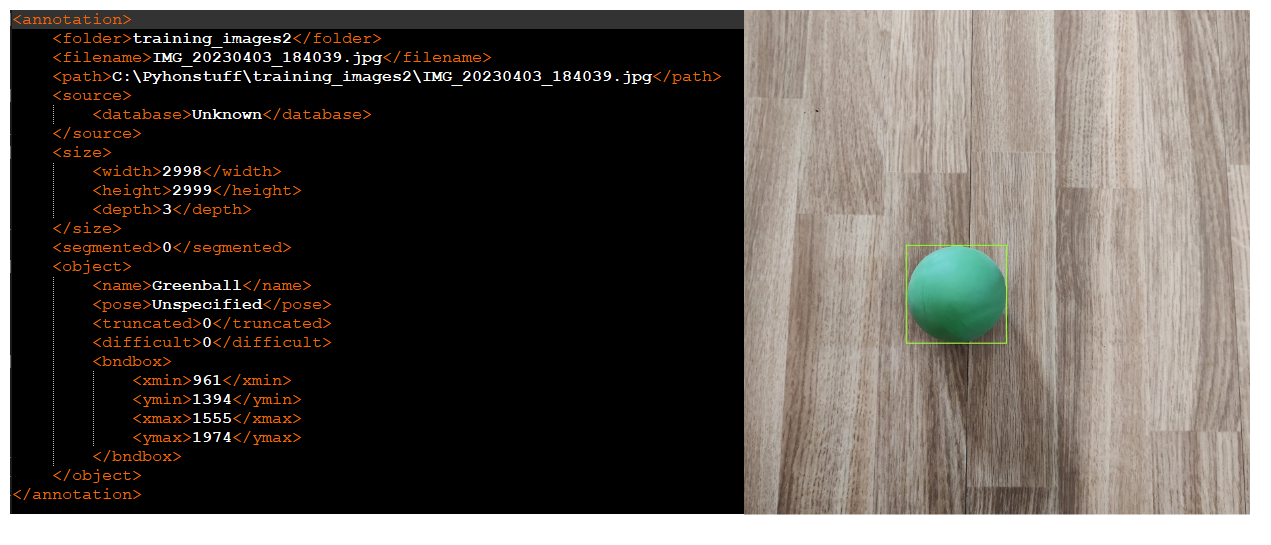
\includegraphics[scale=0.3]{a_martinbilder/pascalvoc_xml.drawio.png}
    \caption{Pascal VOC .xml contents (left), corresponding image (right)}
    \label{fig:pascalvoc}
\end{figure}

The annotated dataset is split into three categories: Training data, validation data and test data. Training data is the set used for training our model. The validation data is used to evaluate the model during the training process. Test data is used to evaluate the final model after training is complete. The final evaluation gives us the model’s precision statistics. The simplicity of Tensorflow Lite Model Maker is best described by the few lines of code required to train a model. Our training script for transfer learning with the EfficientDet Lite1 model can be found in \ref{appendix:ModelMaker}. When the Tensorflow Lite model is trained it needs to be compiled for the TPU. The compilation is done using the Edge TPU Compiler tool which can run on any Linux machine \cite{edgetpuCompiler}


\subsubsection{High level data flow}


Figure \ref{fig:config2_sw} shows the input and outputs of the Tensorflow Lite interpreter object which contains all the methods used to handle inference.
The picamera2 python library provides an interface to the Raspberry Pi camera drivers and allows us to capture image frames as multidimensional arrays. The tflite{\_}interpreter class provides methods for setting up and running inference with our trained object detection model. The model takes the image array as input and outputs the coordinates of bounding boxes around any detected object as well as a prediction score per detected object. The score describes how likely it is that the detection is a true positive. The full source code for configuration 2 can be found in appendix \ref{appendix:NodeCode}\\

\begin{figure}[H]
    \centering
    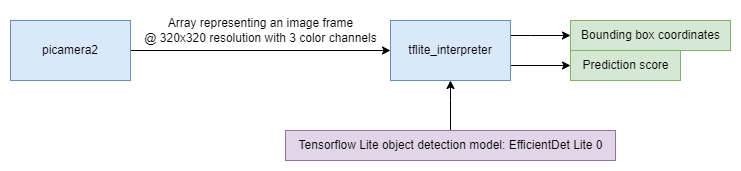
\includegraphics[scale=0.5]{fig/config_2_3_software_highlevel.drawio.png}
    \caption{Software, config 2}
    \label{fig:config2_sw}
\end{figure}

\subsubsection{Reflections}
This section covers aspects of configuration 3 we would have liked to explore further, if given the time.\\
\begin{itemize}
\item \textbf{Camera choice:} EfficientDet Lite 0 and 1 take input images in the sizes 320x320 and 384x384 respectively. Capturing video at resolutions above these values are a waste of resources. We should have used a camera with the ability to capture at low res with a high Field of View. Pi Camera V2 can capture at 640x480, but at this resolution the field of view is severely limited\cite{picameraFOV}. This issue could likely be resolved by using a different camera, unfortunately it was an issue we discovered very late in the project.
\item \textbf{Models:} Getting the YOLOv5 model used in configuration 1 to run on the TPU would result in a better comparison between the two.
\item \textbf{Multi TPU setup:} We only purchased one TPU which left us unable to explore the effects of a multi TPU setup. The Edge TPU Compiler can compile models in segments, each segment then runs on an individual TPU increasing the total throughput.
\end{itemize}




\subsection{Configuration 3, Pi Zero w/ Coral Edge TPU}

\begin{figure}[H]
    \centering
    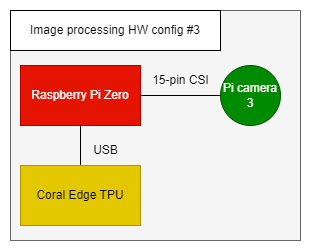
\includegraphics[scale=0.5]{fig/config3_hw.png}
    \caption{Hardware architecture, config 3}
    \label{fig:config3_hw}
\end{figure}

\subsubsection{Software}

Configuration 3 runs the same software as configuration 2.

\subsection{Configuration 4, Pi 4}

\begin{figure}[h]
    \centering
    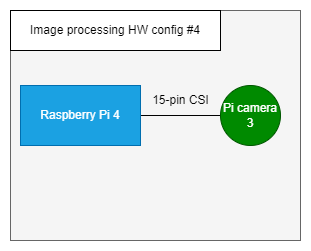
\includegraphics[scale=0.5]{fig/config4_hw.png}
    \caption{Hardware architecture, config 4}
    \label{fig:config4_hw}
\end{figure}

In this section, we will present Configuration 4, which stands out as the sole configuration that does not incorporate hardware acceleration, unlike the other configurations discussed in this report.

\subsubsection{Blob detection software}

For image capture, we use the Pi Camera V3, interfaced via the Picamera2 library. And for image processing, we implement OpenCV \cite{OpenCVDoc}, a widely-used library known for its powerful computer vision and image processing capabilities. It is particularly suitable for blob detection because of its versatility, efficiency, and ease of use. We also used a helper library, cvzone \cite{CVzoneDoc}, to reduce code and complexity. 

\subsubsection{Blob detection models and techniques}

We opted for blob detection or blob analysis \cite{OpenCVBlob}, an image processing technique that identifies and analyzes distinct areas of interest within an image. In the context of our project, blob detection was tasked with identifying balls of different colors.

Blob detection was chosen for its adaptability and precision. It can be finely tuned to detect specific objects, has a high degree of flexibility to meet different computational needs, and is particularly suited to the Raspberry Pi 4's limited processing power. These attributes made blob detection a compelling choice, as our project's aim was to balance detection accuracy with computational efficiency.

To identify the desired objects, our blob detection algorithm utilizes the HSV color space\cite{HSV}, which separates the hue, saturation, and value/brightness components of an image. By selecting appropriate color ranges, we are able to isolate specific objects based on their distinctive color properties.\cite{OpenCVBlob} Once we have found a colored object through color-based detection, our algorithm employs mathematical equations to analyze the contour properties of these objects. Specifically, we determine whether the contours of the detected blobs exhibit circular characteristics. This step helps differentiate the desired balls from other shapes or artifacts in the image. \cite{OpenCVContours}

Blob detection offers a high level of modifiability, allowing it to be tailored to meet specific computational requirements. By adjusting key parameters, the algorithm can be implemented with minimal computational resources, making it suitable for applications where processing power is limited. Alternatively, a larger set of parameters can be utilized, enabling more intricate analysis and detection of complex blobs. However, it should be noted that this approach requires higher computational resources. 

Considering the limitations of the Raspberry Pi 4 without acceleration hardware, the modifiability of blob detection allows us to strike a balance between detection accuracy and computational efficiency. We can optimize the algorithm by fine-tuning parameters to ensure reliable performance on this hardware platform. 

\subsubsection{Software overview}

Camera interface: Picamera2 Python library\\
Object detector type: Blob detection algorithm\\
Image processing library: OpenCV and cvzone\\
Model input: Images from Pi Camera V3\\
Model output: Coordinates of HSV color values and contour properties (circle)\\

OpenCV and our blob detection algorithm process these frames to identify distinct blobs (regions of interest) within the image. The algorithm outputs the coordinates of detected blobs, along with their HSV color values and contour properties. 

\subsubsection{Config4 journey}

\begin{figure}[H]
    \centering
    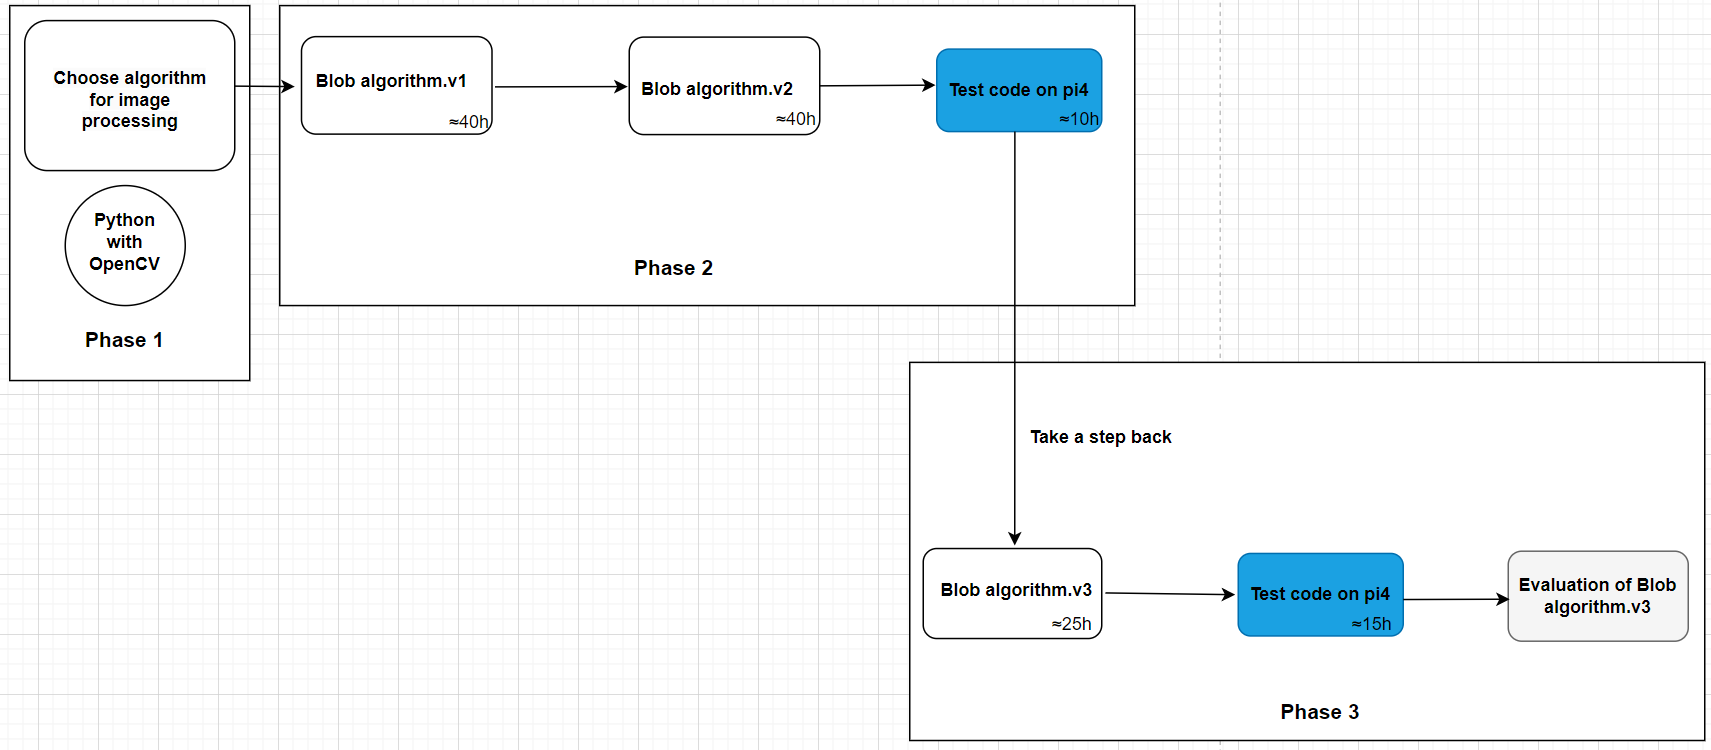
\includegraphics[scale=0.5]{fig/config4model.png}
    \caption{Config model, config 4}
    \label{fig:config4_model}
\end{figure}

To provide a clear and comprehensive understanding of our journey through this configuration, we developed a model accompanied by an explanatory guide. The model is divided into three phases, which illustrate the different stages of our work, the problems we encountered, and the solutions we implemented. This approach offers a better view of how our project developed from start to finish. 

In the first phase of our task, we decided to use Python with OpenCV for image processing. Python is a flexible and user-friendly language, making it an ideal choice for quick development. OpenCV is a powerful tool for image processing, offering a wide range of optimized algorithms. Using Python and OpenCV together enabled us to build and test our image-processing algorithms efficiently and effectively. 

After deciding to use Python and OpenCV for image processing, we needed to choose a suitable algorithm for our task. We selected blob detection, considering its efficiency and simplicity. This algorithm was an easy choice due to the lack of computing resources in our configuration. It’s important to note that efficiency and effectiveness can still depend on the specifics of a task. 

Moving to the second phase, we knew one of our client's wishes was for us to develop a program capable of detecting three tennis-sized balls, each of a different color. The program was also required to calculate and display their x, and y coordinates, the distance of each detected ball, and FPS on the frame. Initially, we worked in such a way that we developed and tested the program on a high-end laptop with a webcam. At this point, our blob detection algorithm could only detect the ball at approximately 1m, when our goal was to detect it up to 3-4m. Here is a picture of how we defined the color range for detection. 

\begin{figure}[H]
    \centering
    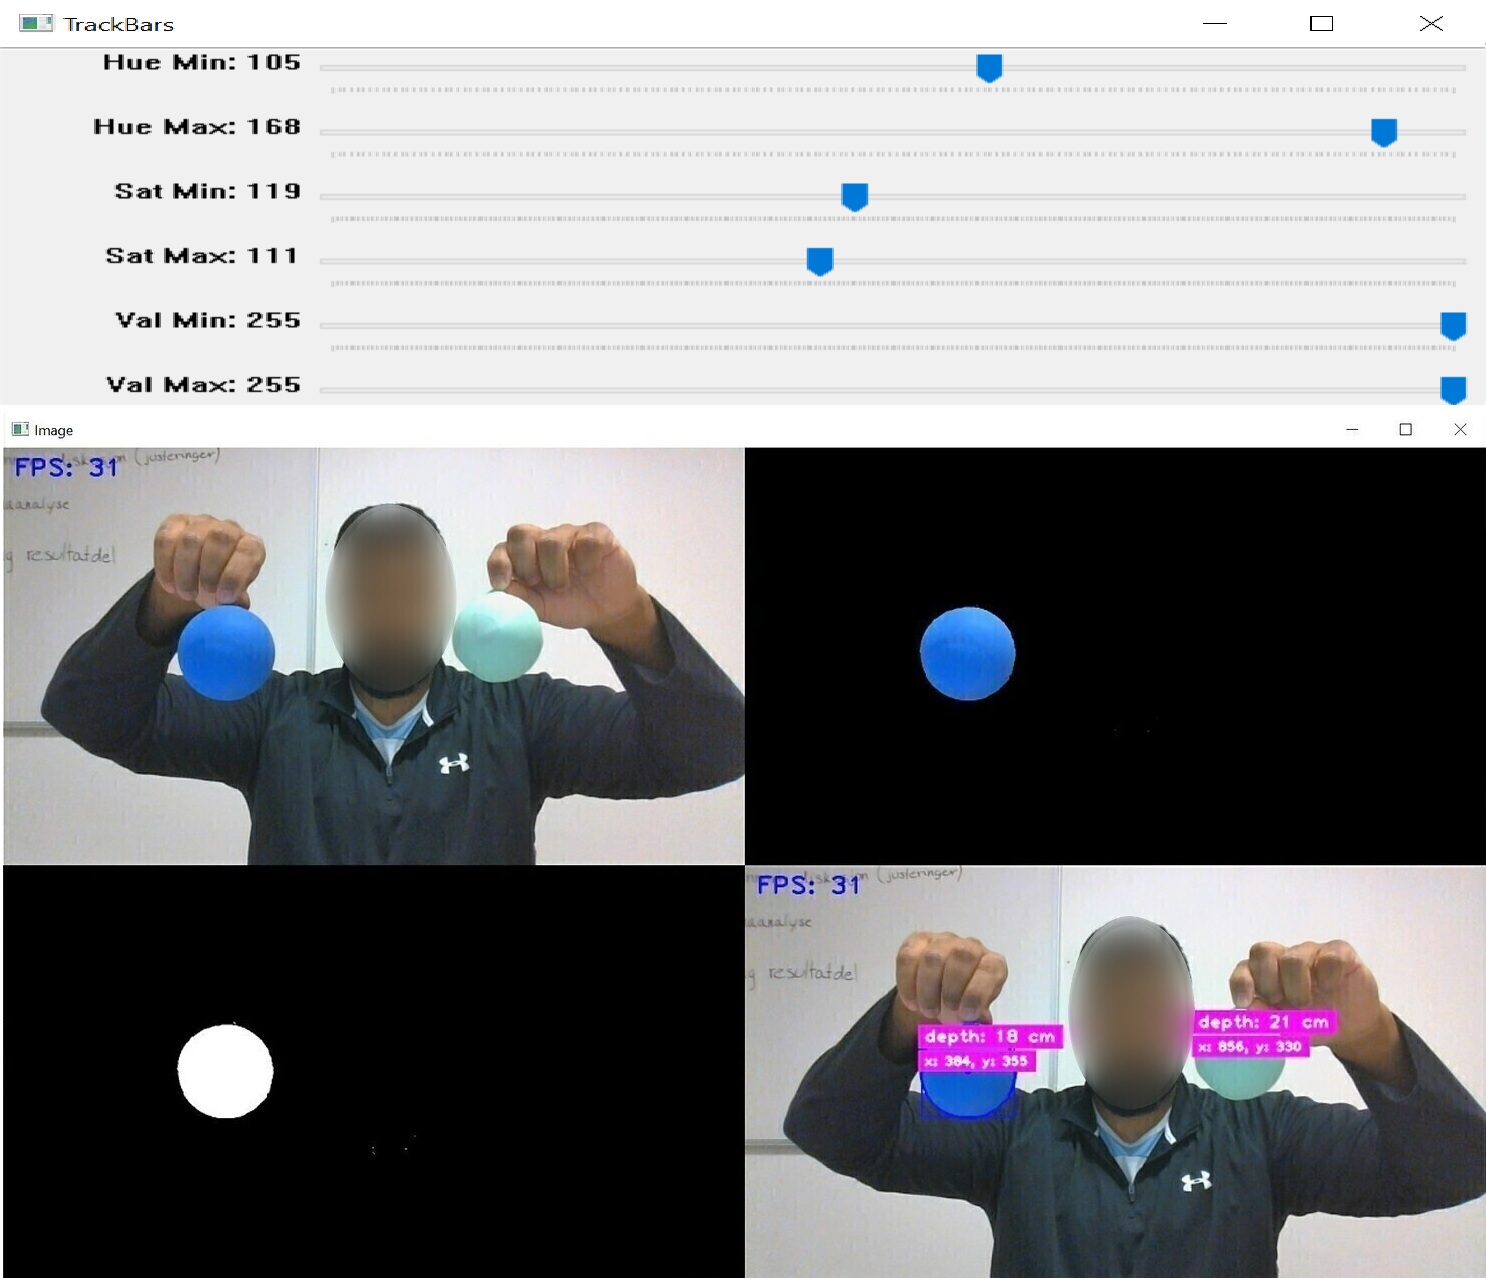
\includegraphics[scale=0.5]{fig/HsvColor.jpg}
    \caption{ColorFinder object, config 4}
    \label{fig:config4_color}
\end{figure}

Having realized that the initial version (Blob detection.v1) \ref{ch:algo} of our program did not fulfill the client's requirement, it became evident that we had to improve our blob detection. As we went to the next step to expand the program's capabilities from detecting one ball to three balls, the computational demands increased, which lead to the challenge of balancing efficiency and performance within our resource constraints.  

With the improvements in place, our v2 version \ref{ch:algo} of the program had advanced to the point where it could successfully detect three differently colored balls, simultaneously displaying their depth along with their x and y coordinates within the frame. However, despite better efficiency and accuracy, we were yet to reach our objective of detecting the balls from a distance of 3-4 meters. Furthermore, the frame rate was still a matter of concern, as we were only able to achieve an average of 4-8 frames per second, varying based on the resolution scale. 

\begin{figure}[H]
    \centering
    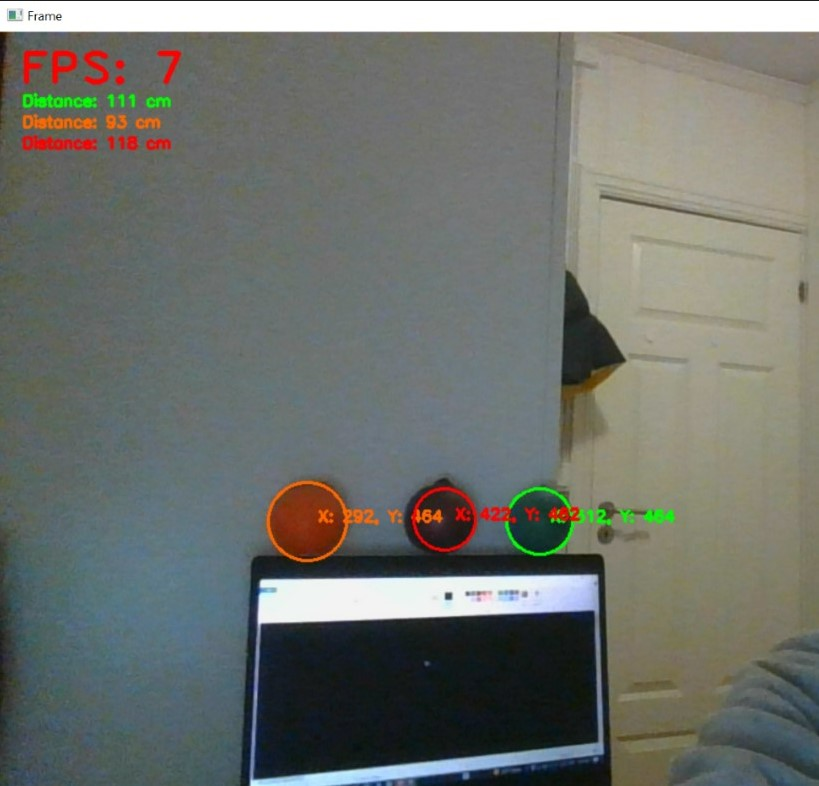
\includegraphics[scale=0.5]{fig/BlobDetection.v2.jpg}
    \caption{BlobDetection.v2, config 4}
    \label{fig:config4_v2}
\end{figure}

Upon testing the program on a Raspberry Pi, we found that the computational demands were too high for the hardware to handle effectively since we built and tested the program on a high-end laptop using the webcam.  As a result, we needed to revisit our approach and develop a more simplified version that could effectively run on the Raspberry Pi. 

In the third phase of our progress, in response to the computational constraints, we developed a simpler blob detection algorithm for the v3 version \ref{ch:algo}. By simplifying and removing some of the more computationally intense functionalities from the program, we were able to finally achieve the detection of the balls from a distance of 3-4 meters on our PC. While the precision of this version was somewhat compromised in comparison to v2, it was a necessary trade-off given our resource constraints. This version also offered a significant improvement in frame rate performance as we were now achieving between 20-25    frames per second, also resolving the previous frame rate issues we had encountered.

Upon testing our code on the Raspberry Pi, we encountered consistent results, primarily due to the frame rate on the desktop PC being limited to 30 fps. Due to the change of cameras being used from webcam to pi camera 3, the HSV values needed to be updated. The code can be modified to be more accurate with further iterations since we see that we can press the raspberry pi even further. 

To further test our configuration, we set out to evaluate the effectiveness of our blob detection. For this purpose, a script was developed to process labeled validation images, calculating precision, recall, and eventually yield the f1 score. This precision metric was chosen to compare our algorithm's performance with a trained model.

The optimal score we achieved was the result of testing over 10,000 different combinations of HSV values:

\begin{figure}[h!]
\centering
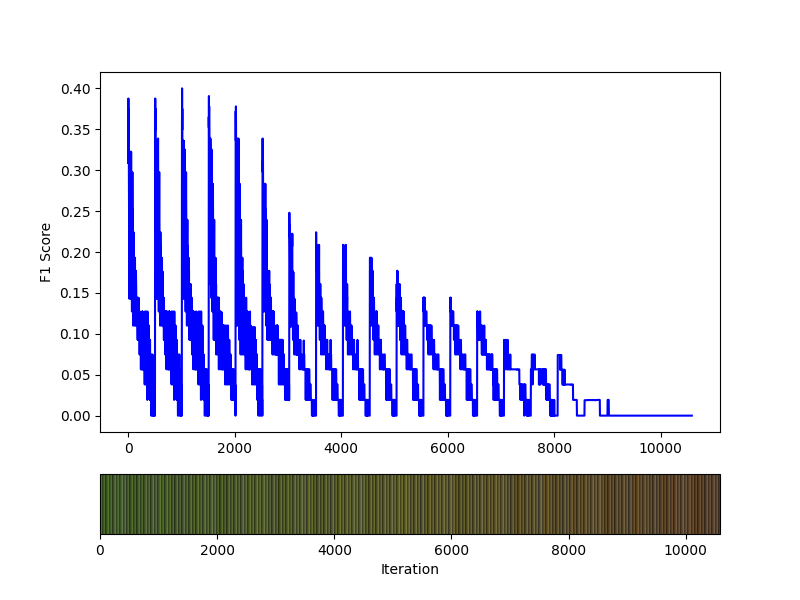
\includegraphics[scale=0.75]{sindrebilder/HSVfinal.png}
\caption{Trying different HSV combinations}
\label{fig:evaluationTest4}
\end{figure}

It's important to clarify that this figure does not aim to showcase the accuracy of our algorithm. Rather, it demonstrates our methodology for optimizing the F1 score across a set of images with varying lighting conditions and environmental factors. \ref{C4evaluation}

However, given the algorithm's dependency on HSV values, its performance varied significantly under different lighting conditions.\cite{Config4Dataset} This was a result of predetermined HSV values becoming inconsistent under varying lighting conditions, leading to inaccurate detections and incomplete detection of objects. To evaluate this, we utilized one image set captured under a wide variety of conditions. The images were taken in different environments, with lighting and distance variables changing extensively. The performance in these assorted conditions yielded varied results, indicating that the image set's robustness under uniform lighting conditions does not necessarily translate to the same level of accuracy under diverse lighting and environmental conditions.

The final test was done on FPS, where we recorded the fps over 30 secounds. This test was done using the ROS architectures and was relativly stable. We had one drop in FPS, but we did not have the time to investigate the manner further.

\subsubsection{Complexity}

While the initial implementation of the blob detection was relatively straightforward, achieving optimal performance was a more intricate process. It required meticulous fine-tuning of parameters to adapt to various conditions, and additional efforts were needed to handle the irregularities present in real-world data.

Maintenance added to the overall complexity, with a recurring need to manually adjust HSV values each time the environment changed. This repetitive process, although not adding significant complexity, was time-consuming and could potentially impact overall system efficiency. It's an area we aim to improve in future iterations of the project.

Despite these complexities, this configuration proved less complex in comparison to others, due largely to fewer encountered difficulties underway.



%\section{Technical overview}

%Our study aims to evaluate and compare four distinct distributed drone architectures, along with one centralized architecture. The distributed architectures solely vary in their approach to image processing. The leftmost diagram in figure \ref{fig:distributed_vs_centralized} illustrates a high-level overview of the four distributed architectures, wherein each box represents hardware with processing capabilities. The rightmost box represents the centralized architecture, where all the processing tasks are performed on a single hardware unit.

\section{Configurations, full context}

In this section, we present our configurations in the full UAV context, from image processing to the flight controller. We will cover ROS2 integration of the image processing modules, and the ROS2 nodes we have developed as we worked towards a complete UAV system.

\subsection{ROS2 integration}

As all image processing modules have the same outputs, the process of integrating them with ROS2 is the same for each module.
An image processing module is split into two nodes which each handle a specific task. One node handles video capture, while the other node handles object detection. The benefit of this modular approach is not obvious for our configurations as both video capture and object detection run on the same hardware. Having the option to run these nodes on dedicated hardware could be useful in the future, which is why we went with the modular approach. An abstract explanation of our nodes can be found in figure \ref{fig:node_description}. For more details see appendix \ref{appendix:NodeCode}, which contains commented code for each node we have developed.

\begin{figure}[h!]
    \centering
    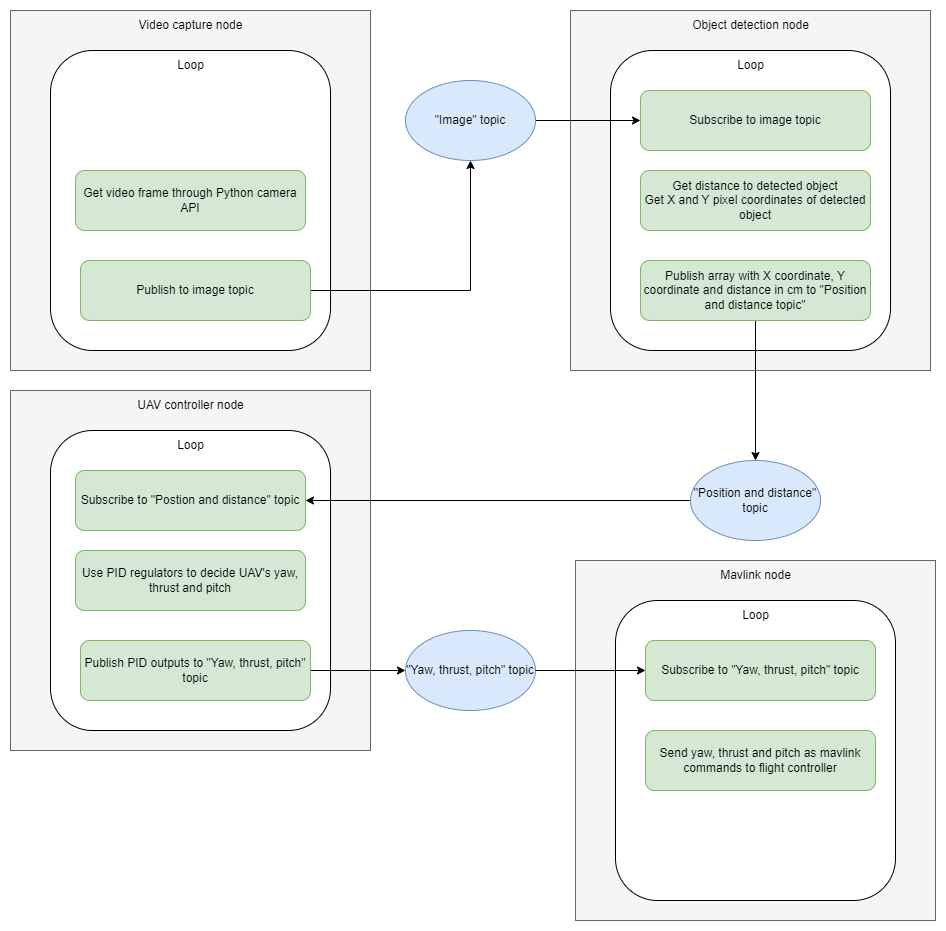
\includegraphics[width=\textwidth]{a_martinbilder/nodes.drawio.png}
    \caption{ROS2 node description}
    \label{fig:node_description}
\end{figure}

\subsection{UAV side project}

Throughout this study we have had ambition to fly a UAV with the ability to follow an object, as mentioned briefly in \ref{sub:accepted_architectures}. The “UAV controller node” and “Mavlink node” in figure \ref{fig:node_description} were made to achieve this goal. Results from real world testing on a UAV would be valuable when comparing the performance of our configurations. Unfortunately, we didn’t reach the point where we could launch a drone with the object following capability. We elaborate on this side project in appendix \ref{drone_impl}




\section{Drone architecture}

\begin{figure}[h]
    \centering
    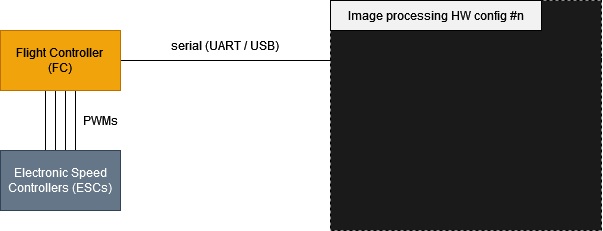
\includegraphics[width=\textwidth]{fig/arch_fc.png}
    \caption{Hardware architecture including the flight controller and ESCs}
    \label{fig:hw_fc}
\end{figure}

The configuration consists of a flight controller flashed with a firmware featuring the ability to receive relatively high-level commands from any image processing-stack and turn it into real, physical movement of a drone.\\
The firmware chosen for this Bachelor's thesis is the "ArduCopter"-firmware from the well-known ArduPilot\cite{documentation-ArduPilot} project, widely regarded as the best open-source flight controller firmware for UAV projects.\cite{firmware-FC} The high-level commands in question being sent is from the widely used MAVLink\cite{documentation-MAVLink} messaging protocol which can be received and transmitted through serial communications (UART / USB).

\subsection{Flight controller firmware setup}
The drone's flight controller has to be flashed with a version of ArduCopter and all necessary calibrations, ESC/motor-setup and tuning can be done through ArduPilot's official Mission Planner-application\cite{documentation-ArduPilot} installed on a desktop computer running Windows or Linux operating system.\\
The flight controller has to also be configured to accept the MAVLink messaging protocol on one of its serial Rx/Tx-ports, which also can be configured through Mission Planner.

\newpage

\subsection{Communication software setup}
The single-board computer in the image processing config-stack needs a way to transmit and recieve MAVLink messages to and from the flight controller. There exists readily available software solutions which can encode MAVLink messages and transmit them over a serial communications interface such as UART or USB.\\\\
Two software solutions were assessed during this Bachelor's thesis:\\
The "Pymavlink" Python-libraries\cite{github-Pymavlink} and the "MAVROS" ROS-package\cite{wiki-MAVROS}.\\\\
While both these solutions were assessed, only "Pymavlink" was actually implemented in a working configuration. This is due to the "MAVROS" ROS-package for the supported ROS 2 distributions (Foxy and Humble) still being in an alpha state\cite{github-MAVROS} as of the time of writing this report, and was therefore omitted.\\
More in-depth information and examples on MAVLink and "Pymavlink" can be found in \ref{MAVLink}.


\newpage

%\subsection{Test bench for distributed architectures}

%This section will cover the commonalities between the distributed architectures. \\

%Figure \ref{fig:dataflow} describes the test setup with internal interfaces. This setup contains all the components needed for a drone with autonomous capabilities, apart from the chassis and actuators which are not needed to measure data processing performance.
%As described in figure \ref{fig:dataflow} all four image processing configurations have the same output format. They publish distance and position data to ROS2 topics which the decision making module subscribes to. This common interface enables testing of the different image processing configurations without making any changes to the remaining modules that make up the drone.




\section{Exploring Use cases}

In this section of the research report, we delve into one of the primary motivations for this project, which is the potential applications of edge computing. Of particular interest is the use case involving drones, which encapsulates the entire spectrum of our work, ranging from the simulation of a drone via the Qualisys motion capture system to the actual construction and piloting of one.

In the following subsections, we will discuss the various tests conducted in our research, along with a detailed analysis of their respective outcomes.

\subsection{Qualisys and drone tracking}
The Qualisys motion capture system is a powerful tool that we use to pinpoint the exact location of the drone. It gives us real-time data on the drone's position in 3D space, with six degrees of freedom (6DOF). This means it can track the drone's movements forward and backward, up and down, left and right, as well as its rotations around three perpendicular axes. With this system, we can monitor and evaluate the drone's position in any environment, including a room. \cite{Qualisys}

\subsubsection{Drone tracking with Qualisys}
Qualisys is exceptionally efficient in tracking drones. It goes beyond merely determining the drone's location; Qualisys supplies accurate tracking data that captures the drone's nuanced movements in real-time. Specifically, we are focused on the yaw, x and y coordinates.
The yaw value helps us understand the drone's rotation around the vertical axis, while the x and y coordinates pinpoint the drone's position in three-dimensional space. By comparing this data with our drone location algorithm's output, we can assess the algorithm's accuracy and reliability. If there are discrepancies, we can refine our algorithm using this high-quality data, ensuring the drone's precise positioning and control.

\subsubsection{Drone position}
In order to calculate the drone position we need to get the distance data (denoted as $d$) from our image processing configurations, and we need to get the yaw (denoted as $\theta$) from the qualisys.
We use the yaw data to simulate magnetometer data we would get from the flightcontroller.
This testing have been done with a dummy drone with qualisys markers on the floor, so that we don't factor in the z axis.

We're essentially using a polar coordinate system with the object at the origin. In this system, a point is described by its distance from the origin, and its angle measured counterclockwise from a reference direction. For our specific problem, this angle is the drone's yaw.

Given this setup, the drone's x ($x_{\text{drone}}$) and y ($y_{\text{drone}}$) positions can be calculated by using trigonometric functions with the distance to the object and the drone's yaw. This calculation assumes that the object is at a location relative to origio, and the drone's yaw is defined as 0 when the drone is north of the object with the camera pointing south, increasing counterclockwise, and decreasing clockwise.

The equations to calculate the drone's position are as follows:

\begin{equation}
x_{\text{drone}} = x_{\text{object}} - d \cdot \sin(\theta)
\end{equation}

\begin{equation}
y_{\text{drone}} = y_{\text{object}} + d \cdot \cos(\theta)
\end{equation}

These equations account for the drone's distance from the object and its orientation. The trigonometric functions sin and cos help to decompose the total distance $d$ into x and y components, providing an estimate for the drone's position. After the estimation, we compare the calculated position with the true position. This allows us to gauge the accuracy of our algorithm. In addition, we plot these positions over time to visually assess the performance of our drone location algorithm.

\subsubsection{Test Results}

With the use of ROS2s get\_logger().info() and the plots generated, we were able to reliably read the test data from our calculations:

\begin{table}[h]
\centering
\resizebox{\textwidth}{!}{%
\begin{tabular}{|c|c|c|c|c|}
\hline
\textbf{Yaw (rad)} & \textbf{Distance to Object (cm)} & \textbf{Estimated Position(x,y)} & \textbf{True Position(x,y)} & \textbf{Difference (\%)}\\ \hline
-0.045 & 92 & (0.0395, 0.919) & (-0.086, 0.941) & 2.65 \\ \hline
1.524 & 88 & (-0.878, 0.0498) & (-0.984, -0.004) & 10.6 \\ \hline
3.015 & 80 & (-0.100, -0.793) & (-0.051, -0.810) & 1.43 \\ \hline
-1.581 & 86 & (0.859, -0.005) & (0.773, -0.017) & 11.1 \\ \hline
\end{tabular}%
}
\caption{Drone Position Testing Data}
\label{tab:qssTest}
\end{table}


The numbers we're discussing are average measurements taken from each yaw, using a still camera. These measurements consider all areas of the coordinate system that our Qualisys tracking system is adjusted to match. We compare our test data with the real coordinates from the Qualisys Tracking Manager (QTM). By finding the distance between each point, we can estimate the difference between them. This test was conducted with the object at the origin point (0,0).

\begin{figure}[!h]
    \centering
    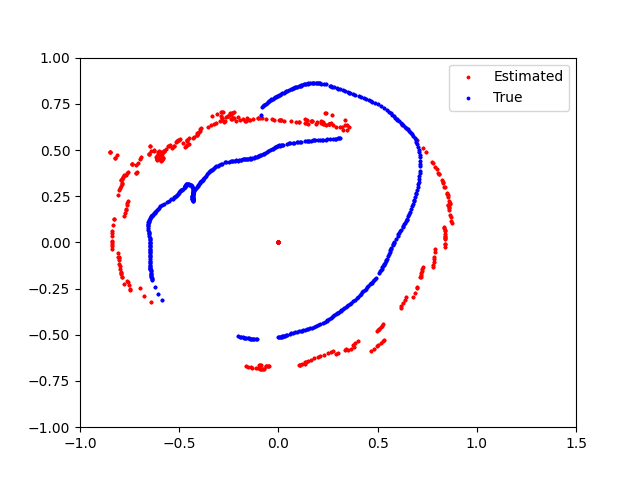
\includegraphics[scale=0.5]{sindrebilder/plotDronefinal.png}
    \caption{Estimated drone position vs Qualisys tracking data}
    \label{fig:qssPlot}
\end{figure}

Data from a moving camera, as shown in \ref{fig:qssPlot}, is not as accurate as the data from a still camera. This might be because the camera was placed half a meter above the ground, something we didn't account for in our tests. Even so, the results indicate that our function is working correctly, which is our main goal.

The testing was done with image processing configuration 4. And since the contours in the frames fluctuate a little from each time, this also factors in on the estimated values. 
\newpage

\subsubsection{ROS1 to ROS2}

The previous project by Local Hawk had utilized Qualisys for drone tracking, and we opted to use their existing codebase. However, this code was designed for ROS1, which required us to convert it to the newer ROS2 standard.

Initially, we contemplated using a bridge between ROS1 and ROS2. However, given that this bridge is still in the alpha phase and only supports standard ROS messages, it was not suited for our application as we were dealing with custom message types developed by Local Hawk. Hence, we decided to translate the ROS-related code from ROS1 to ROS2. We did not make any big changes to the calculations, other than setting some initial values, due to errors parsing the data into the calculation function.

A significant portion of the changes we made were the underlying architecture and methodology of ROS2, which diverges significantly from its predecessor.

The API client library has been changed, and they changed the architecture to be more object-oriented in ROS2. So everything from simple syntax to architecture have been changed. But most of the time was understanding how the ROS1 script worked.

One main challenge arose due to the Qualisys Tracking Manager (QTM) library's dependency on "Asyncio". Both Asyncio and ROS utilize event loops, which manage and distribute the execution of different tasks in an asynchronous programming environment.

This meant we needed to learn how the Asyncio event loop worked to understand what changes had been made. Essentially, these event loops allow multiple tasks to be executed concurrently, without the need for multi-threading or multi-processing. They achieve this by running one task until it needs to wait for an external event (like an I/O operation), then pausing that task and running another. This allows the program to utilize CPU time efficiently, as it can continue processing other tasks while waiting for the external event, instead of just sitting idle.\cite{loopRTS} \newpage

Instead of using the ROS2 spin function, we put the node into the Asyncio event loop. The Local Hawk team started this, but we had to change some parts of the code. You can see these changes in our code breakdown \hyperref[ch:ros1toros2]{here}.


\chapter{Measurements}
\label{ch:Measurements}
\section*{Performance Measurement Results}

The purpose of this section is to evaluate and compare the performance of the four different hardware configurations. This assessment will help us determine the most suitable configuration for achieving the desired balance between processing power, accuracy, and energy efficiency.\\


\textbf{Detection accuracy (precision, recall, F1-score)}
\begin{itemize}

\item Precision: Precision is a measure of how many of the detected objects are actually relevant. It is calculated as the number of true positives (TP) divided by the sum of true positives and false positives (FP). A high precision indicates that the object detection system is good at identifying relevant objects while avoiding false detections. 
Precision = TP / (TP + FP)

\item Recall: Recall is a measure of how many of the relevant objects are detected by the system. It is calculated as the number of true positives (TP) divided by the sum of true positives and false negatives (FN). A high recall indicates that the object detection system is good at finding all the relevant objects in the scene.
Recall = TP / (TP + FN)

\item F1-score: The F1-score is the harmonic mean of precision and recall, providing a single metric that balances both precision and recall. This is useful when you want to compare the performance of different object detection systems, especially when there's a trade-off between precision and recall. An F1-score closer to 1 indicates a better-performing object detection system.
F1-score = 2 * (Precision * Recall) / (Precision + Recall) \cite{preandrec}[p. 155-156]\\ 
\end{itemize}
\newpage
\textbf{Frame Rate}
\begin{itemize}
\item Frame Rate, often measured in frames per second (fps), refers to the speed at which the system can process consecutive images for object detection. It represents the number of images the system can analyze and generate object detection results for within a second.
\item Higher frame rates indicate better performance, as the system can analyze more images in a given period. This is particularly important for drone applications, where real-time or near-real-time object detection is crucial for seamless operation and rapid decision-making.\\
\end{itemize}

\textbf{Power consumption}
\begin{itemize}
 \item Power consumption refers to the amount of electrical power used by the edge configurations while performing object detection tasks. It is measured in watts (W) and is obtained by monitoring the current and voltage supplied to the device during operation.
\item Lower power consumption is generally more desirable, as it indicates higher energy efficiency and can result in longer flight times for the drone. Comparing the power consumption of the four configurations can help determine which option is better suited for a lightweight drone, where battery life and weight are critical factors.\\
\end{itemize}

\textbf{Weight Efficiency}
\begin{itemize}
    \item Weight efficiency refers to the total weight of the configuration, including the computational hardware (like the Jetson Nano or Raspberry Pi), any attached accelerators (like the Google Coral TPU), and necessary components for their function (like heat sinks, cables, power supply, etc.). In the context of drones, lower weight is preferable as it can lead to longer flight times and improved maneuverability. \\
\end{itemize}

\textbf{Complexity (Ease of Setup and Operation)}
\begin{itemize}
\item Complexity in this context refers to the level of difficulty involved in setting up and operating the object detection system. This includes tasks such as installing and configuring the necessary software, implementing the object detection model, troubleshooting issues, and managing the system during operation.
\item 1 represents a very complex system that is difficult to set up and operate. This might include challenges such as complicated installation procedures, hard-to-resolve errors, poor documentation, a steep learning curve, and significant maintenance requirements.
\item 10 represents an easy-to-use system that is straightforward to set up and operate. This might include factors such as clear and thorough documentation, simple installation procedures, easy-to-use tools and interfaces, minimal troubleshooting requirements, and low maintenance needs.\\
\end{itemize}

\textbf{Results}
\begin{table}[ht]
\centering
\begin{tabular}
{ |c|c|c|c|c|c|c|c| } 
\hline
Configuration & config 1 & config 1 & config 2 & config 2 & config 3 & config 3 & config 4\\
              & yolov5n & yolov5s  &  edl0    &  edl1     & edl0    & edl1     & blob\\
\hline
Precision & 0.991 & 0.995 & 0.945 & 0.924 & 0.945 &  0.924 & 0.96\\
\hline
Recall & 1.00 & 1.00 & 0.516 & 0.580 & 0.516 & 0.580 & 0.25\\
\hline
F1-score & 0.96 & 0.96 & 0.667 & 0.712 & 0.667 & 0.712 & 0.399\\
\hline
Avg FPS over 30 sec & 11.03 & 5.966 & 24.64 & 16.46 & 5.70 & 3.92 & 23.33\\
\hline
Power Consumption (W) & 10.8 &  & 11.7 & & 11.7 & & 7,2 W \\
\hline
Weight (g) & 246.1 &  & 87.6 & & 43.3 & & 51.1 \\
\hline
Complexity & 2 &  & 9 & & 9 & & 7 \\
\hline
Price & 124\$ &  & 145\$ & & 100\$ & & 85\$ \\
\hline
\end{tabular}
\caption{Results}
\label{tab:målinger}
\end{table}

\newpage


\begin{figure}[h]
    \centering
    \begin{subfigure}{0.45\textwidth}
        \centering
        \includegraphics[width=\linewidth]{evenbilder/spiderdiag/config1.png}
        \caption{Config 1 results}
        \label{fig:a}
    \end{subfigure}
    \hfill
    \begin{subfigure}{0.45\textwidth}
        \centering
        \includegraphics[width=\linewidth]{evenbilder/spiderdiag/config2.png}
        \caption{Config 2 results}
        \label{fig:b}
    \end{subfigure}
    \\ % this line break will put the next two images on the next line
    \begin{subfigure}{0.45\textwidth}
        \centering
        \includegraphics[width=\linewidth]{evenbilder/spiderdiag/config3.png}
        \caption{Config 3 results}
        \label{fig:c}
    \end{subfigure}
    \hfill
    \begin{subfigure}{0.45\textwidth}
        \centering
        \includegraphics[width=\linewidth]{evenbilder/spiderdiag/config4.png}
        \caption{Config 4 results}
        \label{fig:d}
    \end{subfigure}
    \caption{Results represented in spider diagrams}
    \label{fig:fourgrid}
\end{figure}

\newpage

\section{Config1}

The following figure show the FPS performance of configuration 1 while running object detection.
We ended up testing two Yolo models, nano and small. 
\begin{figure}[H]
    \centering
    \includegraphics[width=\textwidth]{evenbilder/Framerate yolo.png}
    \caption{Yolov5 nano versus small model FPS}
    \label{fig:yolofps}
\end{figure}


\section{Config2 \& Config3}

Both the EfficientDet Lite 0 and EfficientDet Lite 1 models has been benchmarked on the following three hardware configurations:
\begin{itemize}
    \item Raspberry Pi 4B       w/ Coral USB Accelerator (Config 2)
    \item Raspberry Pi Zero2    w/ Coral USB Accelerator (Config 3)
    \item Raspberry Pi 3B+      w/ Coral USB Accelerator
\end{itemize}

All three hardware configurations has been benchmarked by running the Docker-container at "benchmark/coral-1xRPi" from the "Aerial-Edge/Drone" repository \cite{github-Aerial-Edge_Drone} with the latest Raspberry Pi OS Lite (64-bit) natively installed on a Class A2 SDXC-card.

\subsection{EfficientDet Lite 0}
\begin{figure}[H]
    \centering
    \includegraphics[width=\textwidth]{fig/plots/EDL0.png}
    \caption{EfficientDet Lite 0 on various Raspberry Pies}
    \label{fig:edl0}
\end{figure}

\newpage

\subsection{EfficientDet Lite 1}
\begin{figure}[H]
    \centering
    \includegraphics[width=\textwidth]{fig/plots/EDL1.png}
    \caption{EfficientDet Lite 1 on various Raspberry Pies}
    \label{fig:edl1}
\end{figure}

\newpage

\begin{figure}[H]
    \centering
    \includegraphics[width=\textwidth]{fig/plots/EDL0_vs_EDL1.png}
    \caption{EfficientDet Lite 0 compared to EfficientDet Lite 1 on Raspberry Pi 4B}
    \label{fig:edl0_vs_edl1}
\end{figure}

\newpage

\subsection{USB 3.0 vs. USB 2.0}

Plugging the Coral USB Accelerator to a USB 2.0-port instead of 3.0-port pretty much halves the frame rate during the object-detection benchmark. This is consistent with the Coral's tech specs\cite{CoralTPU} which claims that the USB Accelerator is compatible with USB 2.0 but the inferencing speed is slower. Note that both the Raspberry Pi 3B+ and Zero 2 only have USB 2.0 ports but the 4B still produces a substantially higher frame rate than these two when it also is connected on USB 2.0.

\begin{figure}[H]
    \centering
    \includegraphics[width=\textwidth]{fig/plots/EDL0-USB_3_vs_2.png}
    \caption{EfficientDet Lite 0, USB 3.0 vs 2.0 on RPi 4B}
    \label{fig:edl0-usb_2_vs_3}
\end{figure}

\begin{figure}[H]
    \centering
    \includegraphics[width=\textwidth]{fig/plots/EDL1-USB_3_vs_2.png}
    \caption{EfficientDet Lite 1, USB 3.0 vs 2.0 on RPi 4B}
    \label{fig:edl1-usb_2_vs_3}
\end{figure}

\newpage

\section{Config4}

The following figure displays the frame per second (FPS) performance of Configuration 4 while tracking a single object over a 30-second interval with our final blob detection: \ref{ros2nodeC4}

\begin{figure}[h]
    \centering
    \includegraphics[width=\textwidth]{sindrebilder/config4_fps.png}
    \caption{FPS, Configuration 4}
    \label{fig:fpsConfig4}
\end{figure}



\chapter{Conclusion}
\label{ch:conclusion}
Our bachelor's project aimed to provide readers with valuable insights into edge image processing for lightweight unmanned aerial vehicles (UAVs). Through our research and experimentation, we successfully achieved object detection capabilities tailored specifically for such UAVs. We utilized four different hardware and software configurations to accomplish this task.

By benchmarking our four configurations, we assessed their respective detection accuracy and frame-per-second (FPS) performance on a single object. This allowed us to comprehensively evaluate the suitability and effectiveness of each configuration for lightweight UAVs in terms of precision and real-time processing capabilities.

Our findings not only contribute to the field of edge image processing but also hold practical significance for the Local Hawk Project and its endeavors. The results highlight the importance of selecting appropriate hardware and software configurations to achieve optimal object detection performance within the constraints of lightweight UAVs.

Furthermore, this project serves as a foundation for future research and development in the area of edge image processing for lightweight UAVs. The insights gained from our study can guide further improvements in detection accuracy and FPS, leading to enhanced capabilities for lightweight UAVs in various domains, including surveillance, monitoring, and search-and-rescue operations.

Overall, our project successfully addresses the goal of providing the reader with knowledge on edge image processing for lightweight UAVs. Through our experimentation and evaluation, we have demonstrated the feasibility and efficacy of object detection using different configurations, thereby contributing to the advancement of lightweight UAV technologies and applications.


%\chapter{Hovedkapitlene}
%\label{ch:main}

%\section{Underkapittel}
%\label{sec:underkappittel}

%<Her følger eksempler på objekter som ofte brukes i en rapport og hvordan de skal nummereres.>

%Under er det en tabell som benevnes \tabref{tab:number} (\LaTeX-kode: \verb#\tabref{tab:number}#). OBS! Legg merke til at tabellteksten skal være på oversiden av tabellen.

%\begin{table}[!ht]
%  \caption{The different number systems}
%  \label{tab:number}
%  \centering
%  \begin{tabular}{|r|l|}
%    \hline
%    7C0 & hexadecimal \\
%    3700 & octal \\ \cline{2-2}
%    11111000000 & binary \\
%    \hline \hline
%    1984 & decimal \\
%    \hline
%  \end{tabular}
%\end{table}

%\section{Enda en underkapittel}
%\label{sec:endaunderkappittel}

%Under følger en figur og medfølgende figurtekst, \figref{fig:usn-logo} (\LaTeX-kode: \verb#\figref{fig:usn-logo}#), som skal plasseres under bildet/figuren. Figuren og figurteksten skal være midtstilt.

%\begin{figure}[!ht]
%  \centering
%  \includegraphics[width=0.8\textwidth]{USN_logo}
%  \caption{Norwegian (bokmål) variant of the USN logo}
%  \label{fig:usn-logo}
%\end{figure}

%\lipsum

%\begin{figure}[!ht]
%  \centering
%  \includegraphics[width=0.8\textwidth]{USN_logo_en}
%  \caption{English variant of the USN logo.}
%  \label{fig:usn-logo-en}
%\end{figure}

%\lipsum[9]

%\chapter{Diskusjon}
%\label{sec:diskusjon}

%<Utfør diskusjonen her>

%The differential forms of Maxwell's equations as found by Heaviside, while completely valid, are now considered somewhat archaic, and have been replaced by the more useful (equivalent) integral forms. Each law is named according to the person(s) who originally discovered the connections represented by the equation. Here are the four equations\eqref{eq:gaussele} to \eqref{eq:max}

%\begin{eqnarray}
%  \text{Gauss' law for electricity:}& \displaystyle \oint{\vec{E}\cdot\mathrm{d}\vec{A}}&=\frac{Q_{enc}}%{\epsilon_0}\label{eq:gaussele}\\
%  \text{Gauss' law for magnetism:}& \displaystyle \oint{\vec{B}\cdot\mathrm{d}\vec{A}}&=0\label{eq:gaussmag}\\
%  \text{Faraday's law:}& \displaystyle\oint{\vec{E}\cdot\mathrm{d}\vec{s}}&=-\frac{\emph{d}\phi_b}{\mathrm{d}t}\label{eq:fara}\\
%  \text{Ampere-Maxwell law:}& \displaystyle\oint{\vec{B}\cdot\mathrm{d}\vec{s}}&=\mu_0\epsilon_0\frac{\emph{d}\phi_e}{\mathrm{d}t}+\mu_0 i_{enc}\label{eq:max}
%\end{eqnarray}

%Note: $\oint$ is used to specify a closed loop integral, also known as a line integral. It simply means that in the calculations, we must go all the way around the loop; we can't stop part way through or the equations won't be valid.

%\chapter{Konklusjon}
%\label{sec:konklusjon}
%<Skriv konklusjonen her>

%\begin{table}[!ht]
% \caption{The weather forecast}
%  \centering
%   \begin{tabular}{| l | l | l | p{5cm} |}
%    \hline
%    Day & Min Temp & Max Temp & Summary \\ \hline
%    Monday & 11C & 22C & A clear day with lots of sunshine.
%    However, the strong breeze will bring down the temperatures. \\ \hline
%    Tuesday & 9C & 19C & Cloudy with rain, across many northern regions. Clear spells
%    across most of Scotland and Northern Ireland,
%    but rain reaching the far northwest. \\ \hline
%    Wednesday & 10C & 21C & Rain will still linger for the morning.
%    Conditions will improve by early afternoon and continue
%    throughout the evening. \\
%    \hline
%    \end{tabular}
%\end{table}


% A dummy command that causes all bibliographyentries to be displayed
% even though there were not cited in the document. Used for demonstration
% purposes only in this template file.
~\nocite{*}

\cleardoublepage

% The bibliography should be displayed here...
%\printbibliography[heading=bibintoc]
% You rather like to call the bibliography "References"? Then use this instead:
\printbibliography[heading=bibintoc, title={References}]


\appendix


%\chapter{Operating System Architecture}
%\label{ch:osarch}
%\section{Operating System Selection Process}

We wanted to ensure that we had the same operating system configuration across all configurations, and to that end we started testing out different distributions to figure out which one would be the best for our purposes.\\

We wanted to make sure we made an informed decision when it came to our platform, and as such we did a number of tests on other operating systems in order to ensure that we made the correct choice.\\

Initially, we decided to eliminate and narrow down our choices, as the amount of Linux distributions available would make this process in itself take up most of our time. So in order to limit the time spent on this task, we decided to select the most common and mainstream Linux distributions, which effectively narrowed it down to Fedora, Ubuntu, and OpenSUSE in addition to the vendor-supplied Raspberry Pi OS. \\

Then we decided to look at what our architecture should look like with the software running on the different hardware configurations and how we would ensure a uniform configuration across all our running systems. A decision was made to run everything within containers, this would ensure that libraries and versions of software running would be identical across all systems. As a container system, we opted to go for Docker, as this is the most used and the most common configuration out there, and it is well supported on all the platforms we evaluated, and our team already had some knowledge of how to best utilize docker to our advantage.  \\

For the software for communicating between the different parts of our system, we opted to use Robot Operating System version 2 (ROS2). This is a ready-to-run turnkey solution for setting up robots or drones, it makes it easy to communicate between different parts of our system, and it is network aware as well as having a communications system between ROS2 instances running within a Docker environment.\\


After deciding which configurations to explore, we started by systematically installing the different distributions on physical hardware, and examining what functionality worked and what did not. From figure \ref{fig:osarch} you can see the different results and what worked and what did not. \\ 

\begin{figure}[h]
    \centering
    \includegraphics[scale=0.5]{fig/decision_os.png}
    \caption{Decision Process OS}
    \label{fig:osarch}
\end{figure}


As indicated in the figure, there were no systems that met all the requirements we had for our software platform, this caused a need to do further research in order to be able to decide which platform we would use going forward. \\

We further narrowed down our choices to Ubuntu or Debian, as these platforms only had one missing dependency, however, we needed to determine which path would yield the best results in contrast to the work needed to fix each system.\\

\begin{figure}[h]
    \centering
    \includegraphics[scale=0.5]{fig/select_dist.png}
    \caption{Decision Process Distribution}
    \label{fig:distselect}
\end{figure}

Debian had the disadvantage of having problems getting ROS2 to work, which has a fairly complicated and extensive build-system, where the documentation can be outdated due to how fast the ROS2 project moves at this point in time. On the other hand, the challenge posed by the Ubuntu system was the absence of driver software for the camera module version 3. \\

As we had limited experience with the ROS2 build system, and documentation on how to manually build and install the software was sparse, we decided to attempt to install the existing driver from Debian in a Ubuntu environment, in order to run ROS2 with camera version 3. \\

We started by cloning the git repository from the Raspberry Pi foundation, where we knew there was a working driver, as our initial tests with Debian showed this to be the case. After cloning the repository we cross-compiled the kernel configuration along with the necessary libraries for installation on our Ubuntu system. \\

After finishing the installation and booting our new kernel, the hardware was detected, but there was no video output. At this point, it was our opinion that we could still get the hardware to function under Ubuntu, as that would be our best course of action at this moment in time. \\

We continued to perform different tests with different configurations, as well as compiling different versions of the Linux kernel, including a vanilla upstream version. When none of these approaches yielded the results we needed, we were forced to re-evaluate our attack vector for this problem.\\

We revisited the drawing board and had a look at running ROS2 on our Debian system, which would provide us access to the camera module 3 driver, and would simplify the deployment of our software. \\

After deciding to attempt a ROS2 compile for Debian, we dove into the documentation for compiling the software on our system, however, this proved less than straightforward and we had numerous challenges attempting to get the software to compile. As an intermediary solution, we found someone who had compiled a Debian package for us on github, but this was from an older build and we could not verify it for our uses, leaving us with the necessary steps to continue to deploy ROS2 while we had an insecure installation with ROS2 for other group members so we could work in parallel and speed up development.\\

After a long period of non-stop work, we were able to compile ROS2 under a Debian system, allowing us access to the camera module 3 and ROS2 on the same computer. After this step was done, we needed to deploy this to a Docker image, allowing us to control the environment and secure a cohesive and uniform platform for our ROS2 source code.\\



However, an unfortunate side-effect of compiling software is that it grows rather large, and after building our Docker system, it had increased in size to 14GB, which was unwieldy for deployment and it posed a challenge to run on the Raspberry Pi Zero. This was sadly nothing we were able to rectify in time before delivering our project, and while it does work in the Raspberry Pi Zero, deployment is slow and prone to create problems if the Zero runs out of memory while pulling the Docker image.\\

\chapter{Hardware}
\label{ch:hardware}
\iffalse
A single-board computer Ż.Ŵ Image processing configurations
TODO: TABELL MED OVERSIKT OVER CONFIGS
Table 8.1: Image processing configurations
Hardware Computer Vision
Software
Weight
Config 1 Nvidia Jetson
Nano, ArduCamŻ.Ŵ Image processing configurations
TODO: TABELL MED OVERSIKT OVER CONFIGS
Table 8.1: Image processing configurations
Hardware Computer Vision
Software
Weight
Config 1 Nvidia Jetson
Nano, ArduCam
Mini
TensorRT,
YOLOv5
...
Config 2 Raspberry Pi 4,
Coral Edge TPU,
Pi Camera 3.0
OpenCV, Tensor-
Flow Lite
...
Config 3 Raspberry Pi Zero
Mini
TensorRT,
YOLOv8
...
Config 2 Raspberry Pi 4,
Coral Edge TPU,
Pi Camera 3.0
OpenCV, Tensor-
Flow Lite
...
Config 3 Raspberry Pi Zero 
\fi

\title{Hardware}
\section{Specification tables for configs}

All values from these tables that are not referenced externally are done by own measuring.\\
The power supply component for the single-board computers has been omitted from these tables due to there being several different options to choose from when supplying power to these boards and not all of them can be covered here.

\subsection{Config 1}

\begin{table}[!htb]
\begin{tabular}{ | >{\raggedright}p{\dimexpr 0.30\linewidth-2\tabcolsep} |
                   >{\raggedleft}p{\dimexpr 0.14\linewidth-2\tabcolsep} |
                   >{\raggedleft}p{\dimexpr 0.14\linewidth-2\tabcolsep} |
                   >{\raggedleft}p{\dimexpr 0.14\linewidth-2\tabcolsep} |
                    >{\raggedleft}p{\dimexpr 0.14\linewidth-2\tabcolsep} |
                   >{\raggedleft\arraybackslash}p{\dimexpr 0.14\linewidth-2\tabcolsep} | } \hline

&\bfseries{MSRP} & \bfseries{Weight} & \bfseries{Volume} & \bfseries{Power} (idle)   & \bfseries{Power (max)}    \\\hline

\bfseries{Jetson Nano}      & \$ 99     & 241 g     & 232 cm$^{3}$  & 5 W       & 10 W      \\\hline
\bfseries{Pi camera 3}      & \$ 25     & 4 g       & 7 cm$^{3}$    & 0,66 W    & 0,83 W    \\\hline
\bfseries{Camera ribbon}    & -         & 1,1 g     & -             & -         & -         \\\hline
\bfseries{SUM}              & \$ 124    & \bfseries{246,1 g}   & \bfseries{239 cm$^{3}$}    & \bfseries{5,7 W}    & \bfseries{10,8 W}    \\\hline
\end{tabular}
\caption{Hardware specification table for Config 1 hardware \cite{Jetson}\cite{specifications-cameras}}
\label{tab:spec_table_Config1}
\end{table}


\subsection{Config 2}

\begin{table}[!htb]
\begin{tabular}{ | >{\raggedright}p{\dimexpr 0.30\linewidth-2\tabcolsep} |
                   >{\raggedleft}p{\dimexpr 0.14\linewidth-2\tabcolsep} |
                   >{\raggedleft}p{\dimexpr 0.14\linewidth-2\tabcolsep} |
                   >{\raggedleft}p{\dimexpr 0.14\linewidth-2\tabcolsep} |
                    >{\raggedleft}p{\dimexpr 0.14\linewidth-2\tabcolsep} |
                   >{\raggedleft\arraybackslash}p{\dimexpr 0.14\linewidth-2\tabcolsep} | } \hline

&\bfseries{MSRP} & \bfseries{Weight} & \bfseries{Volume} & \bfseries{Power} (idle)   & \bfseries{Power (max)}    \\\hline

\bfseries{Raspberry Pi 4B 4GB}  & \$ 60     & 46 g      & 86 cm$^{3}$   & 2,7 W     & 6,4 W     \\\hline
\bfseries{Pi camera 3}          & \$ 25     & 4 g       & 7 cm$^{3}$    & 0,66 W    & 0,83 W    \\\hline
\bfseries{Camera ribbon}        & -         & 1,1 g     & -             & -         & -         \\\hline
\bfseries{Coral USB}            & \$ 60     & 19,7 g    & 15,6 cm$^{3}$ & 2,5 W     & 4,5 W     \\\hline
\bfseries{USB C-A cable}        & -         & 16,8 g    & -             & -         & -         \\\hline
\bfseries{SUM}                  & \$ 145 & \bfseries{87,6 g}   & \bfseries{109 cm$^{3}$}    & \bfseries{5,7 W}    & \bfseries{11,7 W}    \\\hline
\end{tabular}
\caption{Hardware specification table for Config 2 hardware \cite{datasheet-RPi4B}\cite{power-consumption-RPi4}\cite{specifications-cameras}\cite{CoralTPU}}
\label{tab:spec_table_Config2}
\end{table}

\newpage

\subsection{Config 3}

\begin{table}[!htb]
\begin{tabular}{ | >{\raggedright}p{\dimexpr 0.30\linewidth-2\tabcolsep} |
                   >{\raggedleft}p{\dimexpr 0.14\linewidth-2\tabcolsep} |
                   >{\raggedleft}p{\dimexpr 0.14\linewidth-2\tabcolsep} |
                   >{\raggedleft}p{\dimexpr 0.14\linewidth-2\tabcolsep} |
                    >{\raggedleft}p{\dimexpr 0.14\linewidth-2\tabcolsep} |
                   >{\raggedleft\arraybackslash}p{\dimexpr 0.14\linewidth-2\tabcolsep} | } \hline

&\bfseries{MSRP} & \bfseries{Weight} & \bfseries{Volume} & \bfseries{Power} (idle)   & \bfseries{Power (max)}    \\\hline

\bfseries{Raspberry Pi Zero2}   & \$ 15     & 11 g      & 9,75 cm$^{3}$     & 0,6 W     & 6,4 W     \\\hline
\bfseries{Pi camera 3}          & \$ 25     & 4 g       & 7 cm$^{3}$        & 0,66 W    & 0,83 W    \\\hline
\bfseries{Camera ribbon}        & -         & 1,1 g     & -                 & -         & -         \\\hline
\bfseries{Coral USB}            & \$ 60     & 19,7 g    & 15,6 cm$^{3}$     & 2,5 W     & 4,5 W     \\\hline
\bfseries{USB C-micro cable}    & -         & 7,5 g     & -                 & -         & -         \\\hline
\bfseries{SUM}                  & \$ 100 & \bfseries{43,3 g}   & \bfseries{32 cm$^{3}$}    & \bfseries{3,8 W}    & \bfseries{11,7 W}    \\\hline
\end{tabular}
\caption{Hardware specification table for Config 3 hardware \cite{datasheet-RPiZero2}\cite{power-consumption-RPiZero2}\cite{specifications-cameras}\cite{CoralTPU}}
\label{tab:spec_table_Config3}
\end{table}



\subsection{Config 4}

\begin{table}[!htb]
\begin{tabular}{ | >{\raggedright}p{\dimexpr 0.30\linewidth-2\tabcolsep} |
                   >{\raggedleft}p{\dimexpr 0.14\linewidth-2\tabcolsep} |
                   >{\raggedleft}p{\dimexpr 0.14\linewidth-2\tabcolsep} |
                   >{\raggedleft}p{\dimexpr 0.14\linewidth-2\tabcolsep} |
                    >{\raggedleft}p{\dimexpr 0.14\linewidth-2\tabcolsep} |
                   >{\raggedleft\arraybackslash}p{\dimexpr 0.14\linewidth-2\tabcolsep} | } \hline

&\bfseries{MSRP} & \bfseries{Weight} & \bfseries{Volume} & \bfseries{Power} (idle)   & \bfseries{Power (max)}    \\\hline

\bfseries{Raspberry Pi 4B}  & \$ 60     & 46 g      & 86 cm$^{3}$   & 2,7 W     & 6,4 W     \\\hline
\bfseries{Pi camera 3}      & \$ 25     & 4 g       & 7 cm$^{3}$    & 0,66 W    & 0,83 W    \\\hline
\bfseries{Camera ribbon}    & -         & 1,1 g     & -             & -         & -         \\\hline
\bfseries{SUM}              & \$ 85 & \bfseries{51,1 g} & \bfseries{93 cm$^{3}$}  & \bfseries{3,4 W}  & \bfseries{7,2 W}    \\\hline

\end{tabular}
\caption{Hardware specification table for Config 4 hardware \cite{datasheet-RPi4B}\cite{power-consumption-RPi4}\cite{specifications-cameras}}
\label{tab:spec_table_Config4}
\end{table}

\subsection{Comparison}

\begin{table}[!htb]
\begin{tabular}{ | >{\raggedright}p{\dimexpr 0.30\linewidth-2\tabcolsep} |
                   >{\raggedleft}p{\dimexpr 0.14\linewidth-2\tabcolsep} |
                   >{\raggedleft}p{\dimexpr 0.14\linewidth-2\tabcolsep} |
                   >{\raggedleft}p{\dimexpr 0.14\linewidth-2\tabcolsep} |
                    >{\raggedleft}p{\dimexpr 0.14\linewidth-2\tabcolsep} |
                   >{\raggedleft\arraybackslash}p{\dimexpr 0.14\linewidth-2\tabcolsep} | } \hline

&\bfseries{MSRP} & \bfseries{Weight} & \bfseries{Volume} & \bfseries{Power} (idle)   & \bfseries{Power (max)}    \\\hline

\bfseries{Config 1}& \$ 124     & 246,1 g   & 239 cm$^{3}$  & 5,7 W     & 10,8 W    \\\hline
\bfseries{Config 2}& \$ 145     & 87,6 g    & 109 cm$^{3}$  & 5,7 W     & 11,7 W    \\\hline
\bfseries{Config 3}& \$ 100    & 43,3 g    & 32 cm$^{3}$   & 3,8 W     & 11,7 W    \\\hline
\bfseries{Config 4}& \$ 85    & 51,1 g    & 93 cm$^{3}$   & 3,4 W     & 7,2 W     \\\hline

\end{tabular}
\caption{Hardware specification table for comparison of all configs}
\label{tab:spec_table_comparison}
\end{table}

\section{Single-board computer (SBC)}

A single-board computer (SBC) is a complete computer built on a single circuit board, with microprocessor(s), memory, input/output (I/O) and other features required of a functional computer. Single-board computers are commonly made as demonstration or development systems, for educational systems, or for use as embedded computer controllers. Many types of home computers or portable computers integrate all their functions onto a single printed circuit board.

Unlike a desktop personal computer, single board computers often do not rely on expansion slots for peripheral functions or expansion. Single board computers have been built using a wide range of microprocessors. Simple designs, such as those built by computer hobbyists, often use static RAM and low-cost 32- or 64-bit processors like ARM. Other types, such as blade servers, would perform similar to a server computer, only in a more compact format. \cite{SBC}

Thanks to the characteristics of SBCs, they are a core hardware component in all of the architectural designs in this comparative study.

\newpage
\begin{table}
\begin{tabular}{ | >{\raggedright}p{\dimexpr 0.19\linewidth-2\tabcolsep} |
                   >{\raggedleft}p{\dimexpr 0.27\linewidth-2\tabcolsep} |
                   >{\raggedleft}p{\dimexpr 0.27\linewidth-2\tabcolsep} |
                   >{\raggedleft\arraybackslash}p{\dimexpr 0.27\linewidth-2\tabcolsep} | } \hline

                            & \centering\bfseries{RPi 4B} & \centering\bfseries{RPi Zero2} & \centering\arraybackslash\bfseries{Jetson Nano}\\\hline
\bfseries{CPU}              & Cortex-A72 @ 1.5GHz       & Cortex-A53 @ 1.0GHz   & Cortex-A57 @ 1.43GHz \\\hline
\bfseries{GPU}              & VideoCore IV @ 500MHz     & VideoCore IV @ 400MHz & 128-core Maxwell @ 921MHz \\\hline
\bfseries{Memory}           & 1 GB - 8 GB               & 512 MB                & 4 GB \\\hline
\bfseries{Video decoding}   & H.264/H.265 (4Kp60)       & H.264 (1080p30)       & H.264/H.265 (4Kp60) \\\hline
\bfseries{Video encoding}   & H.264/H.265 (1080p30)     & H.264 (1080p30)       & H.264/H.265 (4Kp30) \\\hline
\bfseries{Connectivity}     & USB 3.0 × 2               & USB 2.0 × 1           & USB 3.0 × 4 \\
                            & USB 2.0 × 2               & UART × 1              & USB 2.0 × 1 \\
                            & UART × 1                  & SPI × 2               & UART × 1 \\
                            & SPI × 2                   & I2C × 1               & SPI × 2 \\
                            & I2C × 1                   &                       & I2C × 3 \\\hline
\bfseries{Form factor}      & 85mm × 56mm               & 65mm × 30mm           & 69mm × 45mm \\\hline
\bfseries{Weight}           & 46g                       & 11g                   & 250g \\\hline
\bfseries{MSRP}             & \$ 35 - \$ 75             & \$ 15                 & \$ 99 \\\hline

\end{tabular}
\caption{Comparison table for single-board computers (SBCs) \protect\cite{datasheet-RPiZero2}\cite{datasheet-RPi4B}\cite{datasheet-JetsonNano}}
\label{tab:comparison_table_SBCs}
\end{table}

When proposing what SBCs to deploy in our test-solution architectures we tend to mainly look at specifications regarding processing power (CPU \& GPU), memory (RAM), hardware-accelerated video encoding/decoding and connectivity (USB, UART etc.) in relation to the weight and form factor of the board. We also need to take into consideration the availability and discrepancy between MSRP and actual sale price due to the current world-wide chip shortage disrupting the market.\\

We decided the top-contenders and implemented them across all configurations:
\begin{itemize}
    \item Raspberry Pi Zero 2 (RPi Zero 2)
    \item Raspberry Pi 4B (RPi 4B)
    \item nVidia Jetson Nano
\end{itemize}

% Fjerne denne? Usikker:
\iffalse
\subsection{nVidia Jetson Nano}
Jetson Nano Developer Kit is a compact, high-performance computer designed to run multiple neural networks simultaneously for applications such as image classification, object detection, segmentation, and speech processing. It enables developers to build AI-powered applications and projects using GPU acceleration. The Jetson Nano comes with a quad-core ARM CPU, NVIDIA GPU with 128 CUDA cores, and 4GB of RAM, making it suitable for applications like robotics, computer vision, and edge computing.\cite{Jetson}

\begin{figure}[h]
    \centering
    \includegraphics[scale=0.3]{fig/JetsonNano-DevKit_Front-Top_Right_trimmed.jpg}
    \caption{Jetson nano \cite{Jetson}}
\end{figure}
\fi


\newpage

\section{Camera}

\begin{table}[!h]
\begin{tabular}{ | >{\raggedright}p{\dimexpr 0.25\linewidth-2\tabcolsep} |
                   >{\raggedleft}p{\dimexpr 0.25\linewidth-2\tabcolsep} |
                   >{\raggedleft}p{\dimexpr 0.25\linewidth-2\tabcolsep} | 
                   >{\raggedleft\arraybackslash}p{\dimexpr 0.25\linewidth-2\tabcolsep} | } \hline

& \centering\bfseries{Camera Module v2}   & \centering\bfseries{Camera Module 3 NoIR}   & \centering\arraybackslash\bfseries{Camera Module 3 Wide} \\\hline
\bfseries{Video Modes}
& 1920 × 1080p47                & 2304 × 1296p56                    & 2304 × 1296p56 \\
& 1640 × 1232p41                & 2304 × 1296p30                    & 2304 × 1296p30 \\
& 640 × 480p206                 & 1536 × 864p120                    & 1536 × 864p120 \\\hline
\bfseries{Focus}
& Adjustable                    & Motorized                         & Motorized  \\\hline
\bfseries{Depth of field}
& Approx 10 cm to ∞             & Approx 10 cm to ∞                 & Approx 5 cm to ∞ \\\hline
\bfseries{Horizontal FoV}
& 62.2 degrees                  & 66 degrees                        & 102 degrees \\\hline
\bfseries{Vertical FoV}
& 48.8 degrees                  & 41 degrees                        & 67 degrees \\\hline
\bfseries{Size}
& 25 × 24 × 9mm                 & 25 × 24 × 11.5mm                  & 25 × 24 × 12.4mm \\\hline
\bfseries{Weight}
& 3g                            & 4g                                & 4g \\\hline
\bfseries{MSRP}
& \$ 25                         & \$ 25                             & \$ 35\\\hline
\end{tabular}
\caption{Comparison table for selected cameras\cite{specifications-cameras}}
\end{table}

\subsection{Rolling vs. Global shutter}
All the cameras selected for this project use a "rolling shutter", meaning each frame of a video is captured not by taking a snapshot of the entire scene at a single instant in time but rather by scanning across the scene rapidly, vertically, horizontally or rotationally. In other words, not all parts of the image of the scene are recorded at exactly the same instant. (Though, during playback, the entire image of the scene is displayed at once, as if it represents a single instant in time.) This produces predictable distortions of fast-moving objects or rapid flashes of light. This is in contrast with "global shutter" in which the entire frame is captured at the same instant. \cite{wikipedia-rolling-shutter}\\
A camera using a "global shutter" would therefore cause less distortion of objects in frame moving very fast, for example in the case of a drone capturing high-speed video footage.

\subsubsection{Raspberry Pi Global Shutter Camera}
Raspberry Pi recently released a new camera during this spring named the "Global Shutter (GS) Camera". The Global Shutter Camera’s image sensor has a 6.3mm diagonal active sensing area, which is similar in size to Raspberry Pi’s HQ Camera. However, the pixels are larger and can collect more light. Large pixel size and low pixel count are valuable in machine-vision applications; the more pixels a sensor produces, the harder it is to process the image in real time. To get around this, many applications downsize and crop images. This is unnecessary with the Global Shutter Camera and the appropriate lens magnification, where the lower resolution and large pixel size mean an image can be captured natively. \cite{documentation-RPi_cameras}\\
The new "GS Camera" would likely work substantially better for the application of capturing video on a drone for object detection, with the only drawback being additional weight from a heavier lens.

\iffalse
\subsection{Pi Camera module v2}
The Raspberry Pi Camera Module v2 was introduced in April 2016 to replace the original Camera Module. The v2 Camera Module is equipped with a Sony IMX219 8-megapixel sensor, which represents a significant upgrade from the 5-megapixel OmniVision OV5647 sensor found in the original camera. The Camera Module is capable of capturing high-definition video and still photographs. It is user-friendly for beginners, but also offers advanced features for users seeking to expand their knowledge. Online examples showcase the camera's versatility for time-lapse, slow-motion, and other video applications, while libraries provided with the camera facilitate the creation of special effects.\\

Further details about the IMX219 and the Exmor R back-illuminated sensor architecture are available on Sony's website, underscoring that the camera's improved resolution represents a leap forward in image quality, color fidelity, and low-light performance. The Camera Module supports 1080p30, 720p60, and VGA90 video modes, in addition to still capture. It attaches via a 15cm ribbon cable to the Camera Serial Interface (CSI) port on the Raspberry Pi, and is compatible with all models of Raspberry Pi 1, 2, and 3. The camera can be accessed through the Multi-Media Abstraction Layer (MMAL) and Video for Linux (V4L) APIs, and numerous third-party libraries are available, such as the Picamera Python library. A "Getting Started with Picamera" resource is available for users seeking guidance on its use. The Camera Module is widely employed in home security applications, as well as in wildlife camera traps.\cite{rpicam2specs}\cite{rpicamspecs}\\


\subsection{Pi Camera module v3}
The Raspberry Pi Camera Module 3 is a compact camera designed by Raspberry Pi, equipped with a 12-megapixel sensor featuring high dynamic range (HDR) and phase detection autofocus. The camera is available in standard and wide-angle variants, both with or without an infrared cut filter.\\

Capable of capturing full HD video and still photographs, the Camera Module 3 includes an HDR mode for up to 3 megapixels. Its operation is fully supported by the libcamera library, and its rapid autofocus feature makes it accessible to beginners while providing ample functionality for advanced users. The Camera Module 3 is compatible with all Raspberry Pi computers and features the same printed circuit board (PCB) size and mounting holes as its predecessor, the Camera Module 2. The only difference in dimension is the height, with the improved optics making the Camera Module 3 several millimetres taller than its predecessor.\cite{rpicam3specs} \\
\fi

\subsection{Camera drivers}
There are currently two different driver libraries for capturing with the Raspberry Pi Cameras:
\begin{itemize}
  \item libcamera \cite{docs-libcamera}
  \item RaspiCam (legacy) \cite{github-raspicam}
\end{itemize}

Some quick benchmark tests indicates that the legacy RaspiCam drivers outperforms the newer libcamera drivers in terms of CPU-usage. The reason for this is likely that the legacy drivers are proprietorially made by the own producer of the Rasberry Pi's GPU-stack (Broadcom) and are therefore more efficiently taking advantage of the hardware.\\\\
Below are screenshots of an RTP-stream, the first using piped output from "libcamera-vid" and the second using "v4l2src", both with a Pi Camera Module v2.\\
The \%CPU usage is over double for the "libcamera-vid" command compared to "v4l2src" when streaming @ 1080p30.

\begin{figure}[!htb]
    \centering
    \includegraphics[width=\textwidth]{fig/gstreamer-libcamera_top_v2.png}
        \caption{libcamera-vid piping video to gstreamer}
\end{figure}

\begin{figure}[!htb]
    \centering
    \includegraphics[width=\textwidth]{fig/gstreamer-raspicam_top_v2.png}
    \caption{v4l2src (RaspiCam) feeding video to gstreamer}
\end{figure}

Unfortunately, the newest Pi Camera Module v3 is not compatible with the legacy RaspiCam drivers.

\section{Hardware Acceleration for ML Inference}

\subsection{Google Coral TPU}
The Coral TPU is a compact, power-efficient chip designed by Google to accelerate TensorFlow Lite models on devices. It enables rapid machine learning processing, enhances data privacy, and eliminates the need for continuous internet connectivity. Developers can achieve high-performance machine learning inferencing, making it an ideal choice for applications like computer vision and natural language processing in various edge devices. \cite{CoralTPU}

\begin{figure}[h]
    \centering
    \includegraphics[scale=0.15]{fig/Coral TPU.jpg}
    \caption{Coral USB accelerator \cite{CoralTPU_bilde}}
\end{figure}

\section{Flight controller}
\label{fc}

When choosing flight controller (FC) board(s) for the hardware stack of our test-solution architectures we tend to mainly look at processor speed and flash memory in relation to form factor and weight as well as the availability in local retail shops. The boards' sensor and connectivity options are aspects we deem less relevant for our research project.

F1, F3, F4, G4, F7, and H7 are the different STM32 processors (aka MCU – Micro Controller Unit). The processor is the brain of a flight controller (FC), similar to the CPU in a computer.

There are currently 11 series of STM32 MCU, from faster to slower processing speeds they are: H7, F7, G4, F4, F3, F2, F1, F0, L4, L1, and L0. \cite{comparison-FC}

We decided to go for a single FC to be used in all the hardware stacks of our test-solution architectures of the latest and greatest generation FC that employs the fastest H7-generation microcontroller unit (MCU) with 2 MB of flash memory. This ensures the drone can run very smoothly and has sufficient flash memory to support any firmware with a full set of features.

\begin{table}
\begin{tabular}{ | >{\raggedright}p{\dimexpr 0.26\linewidth-2\tabcolsep} |
                   >{\raggedleft}p{\dimexpr 0.25\linewidth-2\tabcolsep} |
                   >{\raggedleft}p{\dimexpr 0.25\linewidth-2\tabcolsep} |
                   >{\raggedleft\arraybackslash}p{\dimexpr 0.24\linewidth-2\tabcolsep} | } \hline

\bfseries{Processor}        & \centering\bfseries{Processor Speed}    & \centering\bfseries{Flash Memory}   & \centering\arraybackslash\bfseries{SRAM} \\\hline
\bfseries{F0 (STM32F051)}   & 48MHz                         & 256KB                     & 32KB  \\\hline
\bfseries{F1 (STM32F103)}   & 72MHZ                         & 128KB                     & 96KB  \\\hline
\bfseries{F3 (STM32F303)}   & 72MHz                         & 256KB                     & 80KB  \\\hline
\bfseries{F4 (STM32F405)}   & 168MHz                        & 1MB                       & 192KB \\\hline
\bfseries{F4 (STM32F411)}   & 100MHz                        & 512KB                     & 128KB \\\hline
\bfseries{G4 (STM32G491)}   & 170MHz                        & 512KB                     & 128KB \\\hline
\bfseries{F7 (STM32F745)}   & 216MHz                        & 1MB                       & 320KB \\\hline
\bfseries{F7 (STM32F722)}   & 216MHz                        & 512KB                     & 256KB \\\hline
\bfseries{F7 (STM32F765)}   & 216MHz                        & 2MB                       & 512KB \\\hline
\bfseries{H7 (STM32H743)}   & 480MHz                        & 2MB                       & 1MB   \\\hline

\end{tabular}
\caption{Comparison table for microcontroller unit (MCU) \protect\cite{comparison-FC}}
\end{table}

We decided we wanted to go for a single FC for the hardware stacks of our test-solution architectures. Employing the "STM32H743" MCU, it ensures the drone can run very smoothly and has sufficient flash memory to support any firmware with a full set of features.

We ended up going for a MATEKSYS Flight Controller H743-SLIM \cite{MateksysH743-SLIM} as it fulfills our criteria and could be readily ordered at the Norwegian online store "elefun.no".

\begin{figure}[!htb]
    \centering
    \includegraphics[width=\textwidth]{fig/H743-SLIM_1.jpg}
    \caption{Showcase of MATEKSYS H743-SLIM, from mateksys.com \protect\cite{MateksysH743-SLIM}}
\end{figure}

\newpage


% Deaktiverer denne:
\iffalse
\subsection{PID controller for autonomous flying}

A proportional–integral–derivative controller (PID controller or three-term controller) is a control loop mechanism employing feedback that is widely used in industrial control systems and a variety of other applications requiring continuously modulated control. A PID controller continuously calculates an error value e(t) as the difference between a desired setpoint (SP) and a measured process variable (PV) and applies a correction based on proportional, integral, and derivative terms (denoted P, I, and D respectively), hence the name. \cite{wiki-PID-controller}

\begin{figure}[!htb]
    \centering
    \includegraphics[width=\textwidth]{fig/PID-controller.png}
    \caption{PID controller, from wikipedia.org \protect\cite{wiki-PID-controller}}
\end{figure}

We believe in this stage of the project that it's possible to employ a PID controller program for real-time calculation of the drone's desired action while fed input data from an object detection program running in parallel.
The PID controller program will then generate MAVLink messages to somehow control the drone. This can possibly be done through MAVLink's Manual Control Protocol.
\fi

\chapter{UAV}
\label{ch:UAV}
\section{Flight controller}\label{firmware}
\subsection{Firmware}
\label{fc-firmware}
Flight controller (FC) firmware is the software that runs on a flight controller and controls the operation of an FPV drone. It affects flight performance and features, and different firmware options offer various advantages and disadvantages for different flying styles and preferences. \cite{firmware-FC}

There are mainly two firmwares \cite{firmware-FC} to choose from for autonomous flying today:
\begin{itemize}
  \item INAV
  \item ArduPilot
\end{itemize}

ArduPilot is perhaps the most popular open-source autopilot software suite. It supports a variety of vehicles, including quadcopters, planes, rovers, ground vehicles, even RC submarines.

ArduPilot is known for its extensive features and customization options, making it a good choice for advanced pilots and developers. It supports both autonomous and manual control modes, GPS waypoint navigation, and various sensors like barometers and magnetometers. \cite{firmware-FC}

\begin{figure}[!htb]
    \centering
    \includegraphics[width=\textwidth]{fig/ardupilot_logo.jpg}
    \caption{ArduPilot logo, from ardupilot.org \protect\cite{documentation-ArduPilot}}
\end{figure}

ArduPilot was chosen as baseline firmware since it is a long-standing open-source project that's well-documented \cite{documentation-ArduPilot} compared to INAV \cite{github-wiki-INAV}. ArduPilot is also the only firmware officially supported by the MATEKSYS Flight Controller H743-SLIM (ref: \ref{fc}) out of these two options.


\subsection{MAVLink}
\label{MAVLink}

MAVLink is a very lightweight messaging protocol for communicating with drones (and between onboard drone components).

MAVLink follows a modern hybrid publish-subscribe and point-to-point design pattern: Data streams are sent / published as topics while configuration sub-protocols such as the mission protocol or parameter protocol are point-to-point with retransmission. \cite{documentation-MAVLink}

\iffalse
As ArduPilot natively supports MAVLink  we wanted to take advantage of this and have employed the MAVLink protocol via a ROS2-node running a program utilizing the "pymavlink" python-libraries for serial communcation between the FC and the SBC.
\fi

\subsubsection{MAVLink Commands}
\label{MAVLink-commands}
With the help of the relatively low-level "Pymavlink" Python-library we're able to send and receive messages to and from an ArduCopter-flashed flight controller. To do this, first import "mavutil" from the "pymavlink" libraries and establish a connection and wait for a heartbeat from the flight controller:
\begin{lstlisting}[language=PythonPlus]
from pymavlink import mavutil

# Tries to establish connection on Raspberry Pi serial UART:
the_connection = mavutil.mavlink_connection("/dev/ttyACM0", baud=57600)
the_connection.wait_heartbeat()
\end{lstlisting}

After "the\_connection" is successfully initialized its from here on possible to communicate with the flight controller.
\newpage
As an example, to command the flight controller to change mode, arm throttle, and take off can be done by encoding each of these three desired commands in each of their respective "COMMAND\_LONG" messages, including all the command's parameters, as per the MAVLink.io\cite{documentation-MAVLink} documentation:
\begin{lstlisting}[language=PythonPlus]
# Sets flight controller flight mode to "GUIDED":
the_connection.mav.command_long_send(
    the_connection.target_system,           # Established after heartbeat
    the_connection.target_component,        # Established after heartbeat
    mavutil.mavlink.MAV_CMD_DO_SET_MODE,    # Command to be sent
    0,                                      # Confirmation bit
    1, 4, 0, 0, 0, 0, 0)                    # The command's 7 parameters

# Arms the throttle to allow for motors to spin:
the_connection.mav.command_long_send(
    the_connection.target_system,
    the_connection.target_component,
    mavutil.mavlink.MAV_CMD_COMPONENT_ARM_DISARM,
    0,
    1, 0, 0, 0, 0, 0, 0)

# Takes off to 5 metres above ground level:
the_connection.mav.command_long_send(
    the_connection.target_system,
    the_connection.target_component,
    mavutil.mavlink.MAV_CMD_NAV_TAKEOFF,
    0,
    0, 0, 0, 0, 0, 0, 5)
\end{lstlisting}

Every MAVLink command has 7 parameters that need to be set, these parameters can be looked up in the MAVLink.io\cite{documentation-MAVLink} documentation for each respective command.

\subsubsection{Manual Control Protocol}
The "MAVLink Commands" example above works fine for programmatically moving the drone on a "macro"-scale where the flight controller has GNSS-signal available. To programmatically move the drone on a "micro"-scale its possible to do this through the "MANUAL\_CONTROL"-message as per the MAVLink.io\cite{documentation-MAVLink} documentation:

\begin{lstlisting}[language=PythonPlus]
# After connection already established and heartbeat recieved:
the_connection.mav.manual_control_send(
    the_connection.target_system,   # Established after heartbeat
    x,                              # Pitch, in range [-1000,1000]
    y,                              # Roll, in range [-1000,1000]
    z,                              # Thrust, in range [-1000,1000]
    r,                              # Yaw, in range [-1000,1000]
    0)                              # Bitfield corresponding to extra
                                    # buttons, not needed and can be
                                    # set to 0 in this case
\end{lstlisting}

Note that the z-value (thrust) is in the range [-1000,1000] where -1000 is full negative thrust, 0 is no thrust and 1000 is full thrust. Most aircraft only operate in the range [0,1000] without any functionality for negative thrust. \\
Also note that the thrust can not be modified through this protocol unless the flight controller is in a flight mode that supports manual control, as per the ArduPilot.org\cite{documentation-ArduPilot} documentation.




\subsection{Drone simulation}
\label{drone_sim}
Simulation is implemented by using a Flight Dynamics Model (FDM) of the vehicle to simulate the physics involved with vehicle movement. It receives inputs from a SITL (Software in the Loop) program running the ArduPilot firmware (which are the firmware’s servo/motor outputs) and outputs vehicle status, position, velocities, etc. that result from those inputs back to the firmware simulation. Just as sensors would in the real world case. \cite{documentation-ArduPilot}

\subsubsection{SITL Simulator (Software in the Loop)}
The SITL simulator allows you to run Plane, Copter, or Rover without any hardware. It is a build of the autopilot code using an ordinary C++ compiler, giving you a native executable that allows you to test the behavior of the code without hardware. \cite{documentation-ArduPilot}

Through simulating the drone's flight controller running ArduPilot and interfacing with it through MAVLink messages we're able to test code in a safe environment before deploying it on a physical drone. With the addition of Gazebo \cite{Gazebo} we can see a 3D-rendering of the drone and its surrounding, making it ideal for controlling the simulated drone on a "micro"-scale.

\begin{figure}[!htb]
    \centering
    \includegraphics[width=\textwidth]{fig/sitl-gazebo.png}
    \caption{SITL with Gazebo}
\end{figure}

\newpage
\newpage

\section{Drone implementation}
\label{drone_impl}

During the project a four-rotor "quadcopter" drone was built as the project's attempt at a real-world implementation, mainly to act as a platform for our proof of concept.\\
Due to time constraints and hardware difficulties, the full context configuration with all the ROS2-nodes could not be tuned properly and therefore not implemented safely. The full context implementation was limited only to simulations with SITL.

\begin{figure}[!htb]
    \centering
    \includegraphics[width=\textwidth]{fig/drone/drone_top.jpg}
    \caption{Photo of drone from top}
\end{figure}

\newpage

\begin{figure}[!htb]
    \centering
    \includegraphics[width=\textwidth]{fig/drone/drone_left.jpg}
    \caption{Photo of drone from left}
\end{figure}

\newpage

\begin{figure}[!htb]
    \centering
    \includegraphics[width=\textwidth]{fig/drone/drone_right.jpg}
    \caption{Photo of drone from right}
\end{figure}

\newpage

\begin{figure}[!htb]
    \centering
    \includegraphics[width=\textwidth]{fig/drone/drone_front.jpg}
    \caption{Photo of drone from front}
\end{figure}

\newpage

\begin{figure}[!htb]
    \centering
    \includegraphics[width=\textwidth]{fig/drone/drone_airshot_3p.png}
    \caption{Photo of a drone hovering in the air}
\end{figure}

\newpage

\begin{figure}[!htb]
    \centering
    \includegraphics[width=\textwidth]{fig/drone/drone_airshot_1p.png}
    \caption{Photo taken from drone's perspective doing object detection}
\end{figure}

\chapter{Config4 Code Explanation and Analysis}
\label{ch:algo}

\section{Blob detection.v1}

Since we use the Raspberry Pi Camera Module v3 and not a depth camera, we need to find a way to find the distance to a known object. We ended up using OpenCV and cvzone. Our approach involves detecting a specific color in the video frames, identifying the contours of the detected object, and then calculating the distance based on the object's apparent size in the image.

First, we import the necessary packages for image processing, numerical operations, and color detection:

\begin{lstlisting}[language=PythonPlus]
import cv2
import cvzone
from cvzone.ColorModule import ColorFinder
import numpy as np
\end{lstlisting}

We create a VideoCapture object (OpenCV) to read video frames from the camera \cite{OpenCVDoc}, and set the capture dimensions to 640x480 pixels \cite{OpenCVDoc}:

\begin{lstlisting}[language=PythonPlus]
cap = cv2.VideoCapture(0)
cap.set(3, 640)
cap.set(4, 480)
\end{lstlisting}

Next, we create a ColorFinder object (cvzone) with automatic color range update turned off \cite{CVzoneDoc}, and define the color range for detection (using predetermined HSV values):

\begin{lstlisting}[language=PythonPlus]
myColorFinder = ColorFinder(False)
hsvVals = {'hmin': 97, 'smin': 21, 'vmin': 23, 'hmax': 125, 'smax': 255, 'vmax': 193}
\end{lstlisting}

In a continuous loop, we read the video frames from the camera (OpenCV) \cite{OpenCVDoc}, detect the specified color range in the image using the ColorFinder object (cvzone) \cite{CVzoneDoc}, and find the contours in the binary mask (cvzone) \cite{CVzoneDoc}:

\begin{lstlisting}[language=PythonPlus]
while True:
    success, img = cap.read()
    imgColor, mask = myColorFinder.update(img, hsvVals)
    imgContour, contours = cvzone.findContours(img, mask)
\end{lstlisting}

When contours are detected, we extract data from the first contour (assumed to be the object of interest) and calculate the distance to the object based on its apparent size in the image. We use the real-world dimensions of the object (in this case, a tennis ball with a width of 6.5 cm) and the camera's focal length to compute the distance:

\begin{lstlisting}[language=PythonPlus]
if contours:
    data = contours[0]['center'][0], h - contours[0]['center'][1], int(contours[0]['area'])
    
    f = 535  # focal length of the camera
    W = 6.5  # real-world width of the tennis ball

    w = np.sqrt(contours[0]['area']/np.pi) * 2  # width of the tennis ball in the image
    d = (W * f) / w  # calculate the distance

    print(d)
\end{lstlisting}

Finally, we display the distance in centimeters on the image (cvzone) \cite{CVzoneDoc} and stack the original image, detected color image, binary mask, and contour image for visualization (cvzone) \cite{CVzoneDoc} this is done for testing purpose:

\begin{lstlisting}[language=PythonPlus]
cvzone.putTextRect(img, f'depth: {int(d)} cm', (contours[0]['center'][0] - 75, contours[0]['center'][1] - 50), scale= 2)
imgStack = cvzone.stackImages([img, imgColor, mask, imgContour], 2, 0.5)
cv2.imshow("Image", imgStack)
cv2.waitKey(1)
\end{lstlisting}

This approach is suitable for objects with known dimensions and relatively uniform color distribution. This testing was used with simple color detection. We can use this function to use the contours of trained models to find the distance as well. \newpage

\section{Blob detection.v2}

This code uses OpenCV \cite{OpenCVDoc} and cvzone \cite{CVzoneDoc} to track and measure the distance of 3 tennis-sized balls with different colors in a live video feed from a webcam.

First, we import the necessary packages:
\begin{lstlisting}[language=PythonPlus]
import cv2 as cv
from cvzone.FPS import FPS
import imutils
import math
import numpy as np
\end{lstlisting}

This function \verb|calculateDistance| is used to calculate the distance from the camera to the object based on the radius of the object in pixels. This calculation is based on similar triangles and the field of view of the camera.
\begin{lstlisting}[language=PythonPlus]
# Function to calculate distance from the object based on its radius in pixels
def calculateDistance(ballRadius_px):
    return int(faktor / ballRadius_px)
\end{lstlisting}

This function \verb|detect_colored_object| uses color-based filtering and shape-based detection to identify and locate the colored ball in the video frame \cite{ColoredObject}. The function uses color filtering to create a mask for pixels within the defined color range and applies the Hough Transform function \cite{OpenCVHoughCircle} on a blurred grayscale version of the frame to detect circles. If a detected circle's center lies within the color mask, the function returns the circle's coordinates and radius\cite{CircleDetection}.
\begin{lstlisting}[language=PythonPlus]
# Function to detect a colored object within a given color range and size
def detect_colored_object(colorLower, colorUpper, min_radius, max_radius):
    mask = cv.inRange(hsv, colorLower, colorUpper)
    
    # Erode the mask to remove noise & Dilate the mask to fill gaps
    mask = cv.erode(mask, None, iterations=2)
    mask = cv.dilate(mask, None, iterations=2)
    
    # Convert the frame to grayscale and apply median blur
    gray = cv.cvtColor(frame, cv.COLOR_BGR2GRAY)
    gray = cv.medianBlur(gray, 5)

    # Detect circles using the Hough transform
    circles = cv.HoughCircles(gray, cv.HOUGH_GRADIENT, 1, 20, param1=100, param2=30,
                              minRadius=min_radius, maxRadius=max_radius)

    # Check if any circles were detected
    if circles is not None:
        circles = np.uint16(np.around(circles))

        for circle in circles[0, :]:
            x, y, radius = circle

            # Check if the circle's center is within the mask's boundaries
            if 0 <= x < mask.shape[1] and 0 <= y < mask.shape[0] and mask[y, x] > 0:
                return (x, y, radius)
    return None
\end{lstlisting}

The function \verb|display_object_info| visualizes \cite{OpenCVDisplay} details such as a circle around the detected object, x, and y coordinates, and estimated distance on the video frame. 
\begin{lstlisting}[language=PythonPlus]
# Function to display information about the detected object on the frame
def display_object_info(frame, x, y, radius, distance, color, text_offset):
    if x is not None and y is not None:
        # Draw a circle around the detected object
        cv.circle(frame, (x, y), radius, color, 2)
        
        # Display the coordinates x and y
        coordinates_text = f"X: {x}, Y: {y}"
        
        # Display the distance text
        distance_text = f"Distance: {distance} cm"
        
        # Put the coordinate text on the frame
        cv.putText(frame, coordinates_text, (x + 10, y), cv.FONT_HERSHEY_SIMPLEX, 0.5, color, 2)
        
        # Put the distance text on the frame
        cv.putText(frame, distance_text, (22, 70 + text_offset), cv.FONT_HERSHEY_SIMPLEX, 0.5, color, 2)
\end{lstlisting}

The \verb|ballRadius| is a variable indicating the radius of the tennis ball, the \verb|cameraFOV| is the camera's field of view, and lastly, the \verb|faktor| is a calculation parameter \cite{CircleParameters} used to determine the distance of the object from the camera. 
\begin{lstlisting}[language=PythonPlus]
ballRadius = 3.25   # cm (radius of the ball)
cameraFOV = 62.2    # degrees (field of view of the camera)
faktor = (1280 / 2) * (ballRadius / math.tan(math.radians(kameraFOV / 2))) # Pixels from center to edge divided by minimum distance from the lens
\end{lstlisting}

For each color, the program attempts to detect an object of that color in the frame \cite{OpenCVIterate}. If an object is found, its properties (coordinates, distance) are updated in the color dictionary. The updated information is then displayed \cite{OpenCVDisplay} on the frame. This process repeats for each frame, enabling real-time tracking.
\begin{lstlisting}[language=PythonPlus]
# Main loop
while True:
    (grabbed, frame) = videoCap.read() # Read a frame from the video capture
    fps, img = fpsreader.update(frame, color=(255, 0, 0)) # Update the FPS overlay on the frame
    frame = imutils.resize(frame, width=1280) # Resize the frame
    hsv = cv.cvtColor(frame, cv.COLOR_BGR2HSV) # Convert the frame to HSV format

    # Initialize x, y, and ballRadius_px values for each color
    for color_info in colors.values():
        color_info['x'] = None
        color_info['y'] = None
        color_info['ballRadius_px'] = None

    # Iterate through the defined colors and detect objects
    for idx, (color_name, color_info) in enumerate(colors.items()):
        # Call the detect_colored_object function to find objects in the frame
        obj = detect_colored_object(color_info['lower'], color_info['upper'], color_info['min_radius'],
                                    color_info['max_radius'])

        if obj: # If an object is detected, get the coordinates and radius, distance
            x, y, ballRadius_px = obj
            distance = kalkulerDistanse(ballRadius_px) 
            
            # Update the color_info dictionary with the new values
            color_info['x'] = x
            color_info['y'] = y
            color_info['ballRadius_px'] = ballRadius_px
            color_info['distance'] = distance
\end{lstlisting}

The \verb|display_object_info| function visually \cite{OpenCVDisplay} presents data about the detected object on the video feed.
\begin{lstlisting}[language=PythonPlus]
# Display information about the detected object on the frame
        display_object_info(frame, color_info['x'], color_info['y'], color_info['ballRadius_px'],
                            color_info.get('distance'), color_info['color'], color_info['text_offset'])

    cv.imshow("Frame", frame)  # Show the frame
\end{lstlisting}
Referring back to the discussion in the 'Configuration 4 Journey' section, it was clear that the computational demands of our program far exceeded the capabilities of the hardware in use, given that the development and testing were conducted on a high-end laptop utilizing a webcam. As a result, we needed to revisit our approach and develop Blob detection.v3. 

\section{Blob detection.v3}
By simplifying and
removing some of the more computationally intense functionalities from the program we developed Blob detection.v3.

First, we import the necessary packages:
\begin{lstlisting}[language=PythonPlus]
import cv2
import cvzone
from cvzone.ColorModule import ColorFinder
from cvzone.FPS import FPS
import numpy as np
\end{lstlisting}

The \verb|is_circle| function checks if a shape is circular enough to be considered a circle. If the shape is "round enough" (the roundness is more than the given threshold, which is set to 0.6), it filters out shapes that are not "round enough".
\begin{lstlisting}[language=PythonPlus]
# Function to check if a contour is a circle
def is_circle(cnt, threshold=0.6):
    area = cv2.contourArea(cnt) # Compute the area of the contour
    perimeter = cv2.arcLength(cnt, True) # Compute the perimeter of the contour
    if perimeter == 0: # If the perimeter is zero, it cannot be a circle, return False
        return False
    circularity = 4 * np.pi * area / (perimeter * perimeter) # Calculate the circularity of the contour
    return circularity >= threshold
\end{lstlisting}


Next, we create a \verb|ColorFinder| object (cvzone) with automatic color range update turned off \cite{CVzoneDoc}, and define the color range for detection using predetermined HSV (Hue, Saturation, Value) values:
\begin{lstlisting}[language=PythonPlus]
myColorFinder: ColorFinder = ColorFinder(False)

# Define the HSV color range for blue, green and orange
hsvValsBlue = {'hmin': 105, 'smin': 168, 'vmin': 119, 'hmax': 111, 'smax': 255, 'vmax': 255} #blue
hsvValsGreen = {'hmin': 76, 'smin': 29, 'vmin': 132, 'hmax': 97, 'smax': 124, 'vmax': 255} #green
hsvValsOrange = {'hmin': 0, 'smin': 120, 'vmin': 120, 'hmax': 20, 'smax': 255, 'vmax': 255} #orange
\end{lstlisting}

Each frame from the camera (OpenCV) \cite{OpenCVDoc}, is read and processed for frame rate, which at first is analyzed to find areas that match the color profiles defined for blue, green, and orange in HSVvalues\cite{CVzoneDoc}, and then analyze these colored areas further to identify contours in those regions. These contours are checked for circularity using the \verb|is_circle| function, thereby extracting contours that are likely to be circles.  
\begin{lstlisting}[language=PythonPlus]
    # Update the color detection for blue, green and orange
    imgColorBlue, mask = myColorFinder.update(img, hsvValsBlue)
    imgColorGreen, maskRed = myColorFinder.update(img, hsvValsGreen)
    imgColorOrange, maskOrange = myColorFinder.update(img, hsvValsOrange)

    # Find contours in blue, green and orange color mask 
    imgContourBlue, contours = cvzone.findContours(img, mask)
    imgContourGreen, contoursRed = cvzone.findContours(img, maskRed)
    imgContourOrange, contoursOrange = cvzone.findContours(img, maskOrange)

    # Filter contours that are circles
    circular_contours_blue = [cnt for cnt in contours if is_circle(cnt['cnt'])]
    circular_contours_green = [cnt for cnt in contoursRed if is_circle(cnt['cnt'])]
    circular_contours_orange = [cnt for cnt in contoursOrange if is_circle(cnt['cnt'])]
\end{lstlisting}

Processes and displays the depth, x-position, and y-position for each detected ball. It iterates over three lists containing circular contours for each color, and checks if there are circular contours detected. If so, it selects the first contour and calculates the depth of the ball using its area and predefined values for focal length and ball width \cite{distanceobject}. It then prints the color of the ball and its depth.
\begin{lstlisting}[language=PythonPlus]
# Process and display depth, x, and y position for each ball
    for color, circular_contours_list in zip(['blue', 'green', 'orange'],
                                             [circular_contours_blue, circular_contours_green, circular_contours_orange]):
        if circular_contours_list:
            cnt = circular_contours_list[0]
            data = cnt['center'][0], h - cnt['center'][1], int(cnt['area'])

            f = 474 #focal length of the camera
            W = 6.5 # real-world width of the tennis ball
            w = np.sqrt(cnt['area'] / np.pi) * 2 # width of the tennis ball in the image
            d = (W * f) / w # calculate the distance
            print(f"{color}: {d}")
\end{lstlisting}

The depth is displayed using \verb|cvzone.putTextRect| function\cite{CVzoneDoc} which adds the text "depth: {int(d)} cm" to the \verb|imgContourBlue| image. The x and y position is also displayed using \verb|cvzone.putTextRect|. \verb|ImgStack| is a stack of the original image, color image with a blue mask, binary mask, and contour image, which is then shown with \verb|cv2.imshow|\cite{CVzoneDoc}.
\begin{lstlisting}[language=PythonPlus]
            # Display depth on the frame
            cvzone.putTextRect(imgContourBlue, f'depth: {int(d)} cm',
                               (cnt['center'][0] - 75, cnt['center'][1] - 50), scale=2)
            # Display x and y position on the frame with more space between depth and position
            cvzone.putTextRect(imgContourBlue, f'x: {cnt["center"][0]}, y: {cnt["center"][1]}',
                               (cnt['center'][0] - 75, cnt['center'][1] - 10), scale=1.5)

    imgStack = cvzone.stackImages([img, imgColorBlue, mask, imgContourBlue], 2, 0.5)
    cv2.imshow("Image", imgStack)
\end{lstlisting}
This version offered a significant improvement in frame rate performance and detection and was further tested on Rasberry Pi. 

\newpage


\newpage
\section{Blob Detection.v3 Evaluation} \label{C4evaluation}

We first import the necessary packages to enable image processing, numerical operations, and color detection:

\begin{lstlisting}[language=PythonPlus]
import cv2
import cvzone
from cvzone.ColorModule import ColorFinder
import numpy as np
import xml.etree.ElementTree as ET
import os
import csv
\end{lstlisting}

The function \verb|is_circle| is created to check if a detected contour is circular or not. We calculate the area and the perimeter of the contour and use these values to calculate the circularity. A threshold is set to determine whether the contour is circular or not:

\begin{lstlisting}[language=PythonPlus]
def is_circle(cnt, threshold=0.6):
    area = cv2.contourArea(cnt)
    perimeter = cv2.arcLength(cnt, True)
    if perimeter == 0:
        return False
    circularity = 4 * np.pi * area / (perimeter * perimeter)
    return circularity >= threshold
\end{lstlisting}

The \verb|parse_label| function is designed to parse label information from an XML file. It extracts the name and bounding box coordinates of an object:

\begin{lstlisting}[language=PythonPlus]
def parse_label(xml_file):
    tree = ET.parse(xml_file)
    root = tree.getroot()

    label = {}
    for obj in root.findall('object'):
        name = obj.find('name').text
        box = obj.find('bndbox')
        xmin = int(box.find('xmin').text)
        xmax = int(box.find('xmax').text)
        ymin = int(box.find('ymin').text)
        ymax = int(box.find('ymax').text)
        
        label[name] = [(xmin, ymin, xmax, ymax)]
    return label
\end{lstlisting}
\newpage
We create the \verb|calculate_f1_score| function to compute the F1 score given precision and recall:\cite{preandrec}[p. 156]

\begin{lstlisting}[language=PythonPlus]
def calculate_f1_score(precision, recall):
    if precision + recall == 0:  # to avoid division by zero
        return 0
    else:
        f1_score = 2 * (precision * recall) / (precision + recall)
        return f1_score
\end{lstlisting}

Next, we define the \verb|read_image| function that simply reads an image from a given path using the OpenCV function \verb|imread|:

\begin{lstlisting}[language=PythonPlus]
def read_image(image_file):
    return cv2.imread(image_file)
\end{lstlisting}

In the \verb|detect_color| function, we detect colors in an image using a pre-defined HSV value range. We then use cvzone's findContours function to find the contours in the binary mask. A filter is applied to only select contours that pass the is\_circle test:

\begin{lstlisting}[language=PythonPlus]
def detect_color(image):
    myColorFinder = ColorFinder(False)
    #hsvVals = {'hmin': 49, 'smin': 69, 'vmin': 17, 'hmax': 108, 'smax': 255, 'vmax': 181} #green
    #hsvVals = {'hmin': 0, 'smin': 42, 'vmin': 0, 'hmax': 20, 'smax': 186, 'vmax': 219} #red
    hsvVals = {'hmin': 87, 'smin': 78, 'vmin': 0, 'hmax': 114, 'smax': 195, 'vmax': 174} #blue
    imgColor, mask = myColorFinder.update(image, hsvVals)
    imgContour, contours = cvzone.findContours(image, mask)

    circular_contours = [cnt for cnt in contours if is_circle(cnt['cnt'])]

    results = []
    if circular_contours:
        for cnt in circular_contours:
            x, y, w, h = cv2.boundingRect(cnt['cnt'])
            results.append(('blue', (x, y, x+w, y+h)))
    return results
\end{lstlisting}
\newpage
The \verb|calculate_iou| function is designed to compute the Intersection over Union (IoU) between two bounding boxes. This metric is commonly used in computer vision tasks to evaluate the accuracy of object detection models: \cite{IoUdoc}

\begin{lstlisting}[language=PythonPlus]
def calculate_iou(box1, box2):
    x1, y1, w1, h1 = box1
    x2, y2, w2, h2 = box2

    xi1 = max(x1, x2)
    yi1 = max(y1, y2)
    xi2 = min(x1 + w1, x2 + w2)
    yi2 = min(y1 + h1, y2 + h2)

    inter_area = max(xi2 - xi1, 0) * max(yi2 - yi1, 0)

    box1_area = w1 * h1
    box2_area = w2 * h2
    union_area = box1_area + box2_area - inter_area

    return inter_area / union_area if union_area > 0 else 0
\end{lstlisting}
\newpage
We define the \verb|calculate_precision_recall| function to compute precision and recall based on predictions and ground truth data. For each prediction, we calculate the maximum IoU with all ground truth boxes of the same color. If this maximum IoU is greater than or equal to a set IoU threshold, it's considered a true positive; otherwise, it's a false positive. False negatives are counted as those ground truth boxes that don't have any corresponding prediction with an IoU greater than or equal to the threshold:\cite{preandrec}[p. 155-156]

\begin{lstlisting}[language=PythonPlus]
def calculate_precision_recall(predictions, ground_truth, iou_threshold=0.5):
    TP = FP = FN = 0

    for image_predictions, image_ground_truth in zip(predictions, ground_truth):
        for pred_color, pred_box in image_predictions:
            if pred_color in image_ground_truth:
                ious = [calculate_iou(pred_box, truth_box) for truth_box in image_ground_truth[pred_color]]
                max_iou = max(ious) if ious else 0

                if max_iou >= iou_threshold:
                    TP += 1
                else:
                    FP += 1
            else:
                FP += 1

        for truth_color, truth_boxes in image_ground_truth.items():
            if truth_color not in [pred_color for pred_color, _ in image_predictions]:
                FN += len(truth_boxes)
            else:
                for truth_box in truth_boxes:
                    ious = [calculate_iou(pred_box, truth_box) for pred_color, pred_box in image_predictions if pred_color == truth_color]
                    max_iou = max(ious) if ious else 0
                    if max_iou < iou_threshold:
                        FN += 1

    precision = TP / (TP + FP) if TP + FP > 0 else 0
    recall = TP / (TP + FN) if TP + FN > 0 else 0

    return precision, recall
\end{lstlisting}
\newpage
In our main procedure, we define paths to our image and label directories, then sort and pair up the corresponding image and label files:

\begin{lstlisting}[language=PythonPlus]
image_dir = '/home/vaffe/RandomStuff/dataset/valid/blue/'
label_dir = '/home/vaffe/RandomStuff/dataset/valid/blue/labels/'

image_files = sorted(os.listdir(image_dir))
label_files = sorted(os.listdir(label_dir))
\end{lstlisting}

The code processes each image file and corresponding label file one by one. It reads the image, detects the color (our function returns the bounding boxes of detected objects), and parses the XML label file to obtain the ground truth bounding boxes. The predictions and ground truth are stored for later evaluation:

\begin{lstlisting}[language=PythonPlus]
for image_file, label_file in zip(image_files, label_files):
    image_path = os.path.join(image_dir, image_file)
    label_path = os.path.join(label_dir, label_file)

    image = read_image(image_path)
    label = parse_label(label_path)

    prediction = detect_color(image)

    predictions.append(prediction)
    ground_truths.append(label)

    print('Predicted: ', prediction)
    print('Ground Truth: ', label)

\end{lstlisting}

Finally, we calculate precision, recall, and F1 score, which are commonly used metrics to evaluate the performance of object detection models:

\begin{lstlisting}[language=PythonPlus]
precision, recall = calculate_precision_recall(predictions, ground_truths)
f1_score = calculate_f1_score(precision, recall)

print('Precision: ', precision)
print('Recall: ', recall)
print('F1 Score: ', f1_score)
\end{lstlisting}

The precision metric quantifies the number of correct positive predictions made, while recall (also known as sensitivity) quantifies the number of correct positive results divided by the number of all relevant samples (all samples that should have been identified as positive). The F1 Score is the harmonic mean of precision and recall and provides a single score that balances both the concerns of precision and recall in one number. \cite{preandrec}[p. 155-156]


%References:

%[1] OpenCV VideoCapture. Retrieved from https://docs.opencv.org/master/d8/dfe/classcv_1_1VideoCapture.html

%[2] OpenCV VideoCapture::set. Retrieved from https://docs.opencv.org/master/d8/dfe/classcv_1_1VideoCapture.html#aa6480e6972ef4c00d74814ec841a2939

%[3] Cvzone. (02.22). ColorModule. Retrieved from  https://github.com/cvzone/cvzone/blob/master/cvzone/ColorModule.py

%[4] Cvzone. (02.22). findContours. Retrieved from https://github.com/cvzone/cvzone/blob/master/cvzone/Utils.py#L81

%[5] Cvzone. (02.22). putTextRect. Retrieved from https://github.com/cvzone/cvzone/blob/master/cvzone/Utils.py#L145

%[6] Cvzone. (02.22). stackImages. Retrieved from https://github.com/cvzone/cvzone/blob/master/cvzone/Utils.py#L12

\chapter{Config4 Source code}
\section{Blob Detection.v1}

\begin{lstlisting}[language=PythonPlus]
import cv2 
import cvzone 
from cvzone.ColorModule import ColorFinder
from cvzone.FPS import FPS  
import numpy as np 

fpsreader = FPS() 
cap = cv2.VideoCapture(0)  
cap.set(3, 640)  
cap.set(4, 480) 

success, img = cap.read()  
h, w, _ = img.shape  

myColorFinder = ColorFinder(False)  
hsvVals = {'hmin': 36, 'smin': 29, 'vmin': 44, 'hmax': 90, 'smax': 150, 'vmax': 187}

while True: 
    success, img = cap.read() 
    fps, img = fpsreader.update(img)
    imgColor, mask = myColorFinder.update(img, hsvVals)
    imgContour, contours = cvzone.findContours(img, mask)  

    if contours:  
        data = contours[0]['center'][0], h - contours[0]['center'][1], int(contours[0]['area'])

        f = 535
        W = 6.5
        w = np.sqrt(contours[0]['area'] / np.pi) * 2
        d = (W * f) / w

        x, y = contours[0]['center'][0], contours[0]['center'][1]

        print("x: ", x)
        print("y: ", y)

        print(fps)

        cvzone.putTextRect(img, f'depth: {int(d)} cm', (contours[0]['center'][0] - 75, contours[0]['center'][1] - 50),
                           scale=2)  
        cv2.putText(img, f'x: {int(x)}, y: {int(y)}', (20, h - 600), cv2.FONT_HERSHEY_SIMPLEX, 1.5, (255, 0, 0),
                    thickness=2)

    imgStack = cvzone.stackImages([img, imgColor, mask, imgContour], 2,
                                  0.5)
    cv2.imshow("Image", imgStack) 

    if cv2.waitKey(1) & 0xFF == ord('q'):
        break
cap.release()
cv2.destroyAllWindows()
\end{lstlisting}

\section{Blob Detection.v2}

\begin{lstlisting}[language=PythonPlus]
import cv2 as cv
from cvzone.FPS import FPS
import imutils
import math
import numpy as np

def calculateDistance(ballRadius_px):
    return int(faktor / ballRadius_px)

def detect_colored_object(colorLower, colorUpper, min_radius, max_radius):
    
    mask = cv.inRange(hsv, colorLower, colorUpper)
    mask = cv.erode(mask, None, iterations=2)
    mask = cv.dilate(mask, None, iterations=2)

    gray = cv.cvtColor(frame, cv.COLOR_BGR2GRAY)
    gray = cv.medianBlur(gray, 5)

    circles = cv.HoughCircles(gray, cv.HOUGH_GRADIENT, 1, 20, param1=100, param2=30,
                              minRadius=min_radius, maxRadius=max_radius)

    if circles is not None:
        circles = np.uint16(np.around(circles))

        for circle in circles[0, :]:
            x, y, radius = circle

            if 0 <= x < mask.shape[1] and 0 <= y < mask.shape[0] and mask[y, x] > 0:
                return (x, y, radius)
    return None

def display_object_info(frame, x, y, radius, distance, color, text_offset):
    if x is not None and y is not None:
       
        cv.circle(frame, (x, y), radius, color, 2)
        coordinates_text = f"X: {x}, Y: {y}"
        distance_text = f"Distance: {distance} cm"

        cv.putText(frame, coordinates_text, (x + 10, y), cv.FONT_HERSHEY_SIMPLEX, 0.5, color, 2)
        cv.putText(frame, distance_text, (22, 70 + text_offset), cv.FONT_HERSHEY_SIMPLEX, 0.5, color, 2)

ballRadius = 3.25   # cm (radius of the ball)
cameraFOV = 62.2    # degrees (field of view of the camera)
faktor = (1280 / 2) * (ballRadius / math.tan(math.radians(kameraFOV / 2)))

colors = {
    'green': {
        'lower': (72, 70, 32), 
        'upper': (99, 244, 107),
        'min_radius': 0, #ex between 0 
        'max_radius': 0, #to ex 60 pixels
        'color': (0, 255, 0), 
        'text_offset': 0, #Distance text position under FPS
    },
    'orange': {
        'lower': (0, 115, 99), 
        'upper': (18, 255, 255), 
        'min_radius': 0,
        'max_radius': 0,
        'color': (0, 102, 255), 
        'text_offset': 20, 
    },
    'red': {
        'lower': (119, 37, 0), 
        'upper': (179, 179, 147), 
        'min_radius': 0,
        'max_radius': 0,
        'color': (0, 0, 255), 
        'text_offset': 40,  
    },
}

fpsreader = FPS() 
videoCap = cv.VideoCapture(0) 
videoCap.set(3, 1280)
videoCap.set(4, 720)

while True:
    (grabbed, frame) = videoCap.read() 
    fps, img = fpsreader.update(frame, color=(255, 0, 0)) 
    frame = imutils.resize(frame, width=1280) 
    hsv = cv.cvtColor(frame, cv.COLOR_BGR2HSV) 

    for color_info in colors.values():
        color_info['x'] = None
        color_info['y'] = None
        color_info['ballRadius_px'] = None

    for idx, (color_name, color_info) in enumerate(colors.items()):
        obj = detect_colored_object(color_info['lower'], color_info['upper'], color_info['min_radius'],
                                    color_info['max_radius'])
        if obj: 
            x, y, ballRadius_px = obj 
            distance = kalkulerDistanse(ballRadius_px) 
            
            color_info['x'] = x
            color_info['y'] = y
            color_info['ballRadius_px'] = ballRadius_px
            color_info['distance'] = distance

        display_object_info(frame, color_info['x'], color_info['y'], color_info['ballRadius_px'],
                            color_info.get('distance'), color_info['color'], color_info['text_offset'])

    cv.imshow("Frame", frame)  
    key = cv.waitKey(1)  
    if key == ord("q"):
        break
\end{lstlisting}

\section{Blob Detection.v3}

\begin{lstlisting}[language=PythonPlus]
import cv2
import cvzone
from cvzone.ColorModule import ColorFinder
from cvzone.FPS import FPS
import numpy as np

def is_circle(cnt, threshold=0.6):
    area = cv2.contourArea(cnt)
    perimeter = cv2.arcLength(cnt, True)
    if perimeter == 0:
        return False
    circularity = 4 * np.pi * area / (perimeter * perimeter)
    return circularity >= threshold

fpsreader = FPS()

cap = cv2.VideoCapture(0)
cap.set(cv2.CAP_PROP_FRAME_WIDTH, 640)
cap.set(cv2.CAP_PROP_FRAME_HEIGHT, 480)

ret, frame = cap.read()
h, w, _ = frame.shape

myColorFinder: ColorFinder = ColorFinder(False)
hsvValsBlue = {'hmin': 105, 'smin': 168, 'vmin': 119, 'hmax': 111, 'smax': 255, 'vmax': 255} 
hsvValsGreen = {'hmin': 76, 'smin': 29, 'vmin': 132, 'hmax': 97, 'smax': 124, 'vmax': 255} 
hsvValsOrange = {'hmin': 0, 'smin': 120, 'vmin': 120, 'hmax': 20, 'smax': 255, 'vmax': 255} 

while True:
    ret, frame = cap.read()  
    fps, img = fpsreader.update(frame)  

    imgColorBlue, mask = myColorFinder.update(img, hsvValsBlue)  
    imgColorGreen, maskRed = myColorFinder.update(img, hsvValsGreen) 
    imgColorOrange, maskOrange = myColorFinder.update(img, hsvValsOrange)  

    imgContourBlue, contours = cvzone.findContours(img, mask)  
    imgContourGreen, contoursRed = cvzone.findContours(img, maskRed)  
    imgContourOrange, contoursOrange = cvzone.findContours(img, maskOrange)

    circular_contours_blue = [cnt for cnt in contours if is_circle(cnt['cnt'])]
    circular_contours_green = [cnt for cnt in contoursRed if is_circle(cnt['cnt'])]
    circular_contours_orange = [cnt for cnt in contoursOrange if is_circle(cnt['cnt'])]

    for color, circular_contours_list in zip(['blue', 'green', 'orange'],
                                             [circular_contours_blue, circular_contours_green, circular_contours_orange]):
        if circular_contours_list:
            cnt = circular_contours_list[0]
            data = cnt['center'][0], h - cnt['center'][1], int(cnt['area'])

            f = 474
            W = 6.5
            w = np.sqrt(cnt['area'] / np.pi) * 2
            d = (W * f) / w
            print(f"{color}: {d}")

            cvzone.putTextRect(imgContourBlue, f'depth: {int(d)} cm',
                               (cnt['center'][0] - 75, cnt['center'][1] - 50), scale=2)
            cvzone.putTextRect(imgContourBlue, f'x: {cnt["center"][0]}, y: {cnt["center"][1]}',
                               (cnt['center'][0] - 75, cnt['center'][1] - 10), scale=1.5)

    imgStack = cvzone.stackImages([img, imgColorBlue, mask, imgContourBlue], 2, 0.5)
    cv2.imshow("Image", imgStack)
    if cv2.waitKey(1) & 0xFF == ord('q'):
        break
cap.release()
cv2.destroyAllWindows()
\end{lstlisting}

\chapter{ROS1 to ROS2}
\label{ch:ros1toros2}
\section{Translating from ROS1 to ROS2}

The following documentation describes our process of translating from ROS1 to ROS2. It's important to note that this translation does not represent an optimal approach. Although improvements could be implemented to enhance the efficiency and readability of the code, the aim of this translation was to ensure compatibility with ROS2, maintaining performance, and providing satisfactory results in the tests we conducted. This document also assumes that the reader have some knowledge about ROS2 or 1.

\subsection{Syntax Changes}

The syntax of ROS1 and ROS2, while largely similar, exhibits several distinctions primarily associated with changes in the architectural structure of scripts. Among the differences, library usage stands out:

\begin{lstlisting}[language=PythonPlus]
#ROS1
import rospy
import rosgraph

#ROS2
import rclpy
from rclpy.node import Node
\end{lstlisting}

In ROS1, rospy and rosgraph serve as the key libraries for node creation and computation graph visualization. Transitioning to ROS2, rclpy replaces these libraries, providing a Python API for ROS2 interactions, with the Node class encapsulating a node within the ROS graph.

Moreover, modifications were also made to logging functions. Despite the changes, the functions retain a similar operational manner:

\begin{lstlisting}[language=PythonPlus]
#ROS1
rospy.loginfo()

#ROS2
get_logger().info()
\end{lstlisting}

\subsection{Architecture}

The most significant modifications involved the creation and architecture of the ROS nodes. In ROS2, a class is established that inherits from the rclpy node class. Within this class, the node is named, and subscribers, publishers, and other necessary variables for the node are added. Subsequently, this node is initialized within the main function:

\begin{lstlisting}[language=PythonPlus]
#ROS2
class Qualisys_node(Node):

    def __init__(self):
        super().__init__('qualisys_node')

        self.pub = self.create_publisher(DronePose, 'drone_pose', 10)

\end{lstlisting}

All the functions that the class will utilize are defined within it, incorporating the \verb|self| parameter for invocations within the class:

\begin{lstlisting}[language=PythonPlus]
#ROS2
class Qualisys_node(Node):

    def __init__(self):
    def talker(self, data):
    def create_msg(self,x,y,z,v_x,v_y,v_z,a_x,a_y,a_z,yaw,v_yaw,freq,full_msg):
    def calculate_vel_a(self,position,freq, yaw):
    def calc(self,position,rot,freq):
    def create_body_index(self, xml_string):
    def get_freq(self, xml_string):
    async def qtmMain(self):

\end{lstlisting}

This stands in contrast to the ROS1 architecture, where an overarching class to manage the functions does not exist. Instead, a main function is utilized that accepts the publisher as a parameter:

\begin{lstlisting}[language=PythonPlus]
#ROS1
async def mainQualisys(pub):

\end{lstlisting}

In ROS1, this main function for the node is what runs indefinitely. Unlike in ROS2, where a class object is initiated to run endlessly. Our modifications to the loops were minor and mainly involved creating variables and tasks:

\begin{lstlisting}[language=PythonPlus]
#ROS1
asyncio.ensure_future(mainQualisys(pub))
asyncio.get_event_loop().run_forever()

#ROS2
loop = asyncio.get_event_loop()
qtm_task = loop.create_task(qtm_node.qtmMain())
...
asyncio.ensure_future(qtm_task)
loop.run_forever()

\end{lstlisting}

Although the main functions in ROS1 and ROS2 might appear different, they operate similarly in that the node is initialized within the main function. However, in ROS1, subscribers and publishers are also created within the main:

\begin{lstlisting}[language=PythonPlus]
#ROS1
if __name__ == "__main__":
    rospy.init_node('qualisys', anonymous=True) #Node initialization
    pub = rospy.Publisher('/drone_controller/current_pos', DronePose, queue_size=10) #create publisher

#ROS2
def main(args=None):
    rclpy.init(args=args) #Node initialization
    qtm_node = Qualisys_node() #Creates Node
\end{lstlisting}

Upon executing the code with these modifications, we encountered some issues with the data received from Qualisys. It was not in the same format as expected by the \verb|create_msg| function. To resolve this issue, we initialized the values outside the class, which corrected the problem of acquiring initial values from Qualisys:

\begin{lstlisting}[language=PythonPlus]
#ROS2
if prev_msg is None:
    prev_msg = DronePose()
    prev_msg.pos.x = 0.0
    prev_msg.pos.y = 0.0
    prev_msg.pos.z = 0.0
    prev_msg.vel.x = 0.0
    prev_msg.vel.y = 0.0
    prev_msg.vel.z = 0.0
    prev_msg.yaw.data = 0.0

if prev_vel is None:
    prev_vel = [0.0, 0.0, 0.0] 

\end{lstlisting}




%\chapter{Configuration 4}
%\label{appendix:config4}
%\section{Blob Detection}

To identify the desired objects, our blob detection algorithm utilizes the HSV color space, which separates the hue, saturation, and value/brightness components of an image. By selecting appropriate color ranges, we are able to isolate specific objects based on their distinctive color properties. Once we have found a colored object through color-based detection, our algorithm employs mathematical equations to analyze the contour properties of these objects. Specifically, we determine whether the contours of the detected blobs exhibit circular characteristics. This step helps differentiate the desired balls from other shapes or artifacts in the image. 

Blob detection offers a high level of modifiability, allowing it to be tailored to meet specific computational requirements. By adjusting key parameters, the algorithm can be implemented with minimal computational resources, making it suitable for applications where processing power is limited. Alternatively, a larger set of parameters can be utilized, enabling more intricate analysis and detection of complex blobs. However, it should be noted that this approach requires higher computational resources. 

Considering the limitations of the Raspberry Pi 4 without acceleration hardware, the modifiability of blob detection allows us to strike a balance between detection accuracy and computational efficiency. We can optimize the algorithm by fine-tuning parameters to ensure reliable performance on this hardware platform. 









\chapter{Yolo training Tutorial}
\label{appendix:Yolo Training Tutorial}
\textbf{Prerequisites}\\

A computer with an NVIDIA graphics card that is CUDA compatible (RTX 2070 was used in this study). Although you can train with a CPU, it will be significantly slower.\\
A virtual environment with Python 3.8 – 3.11 (Python 3.9.16 was used in this study).

\begin{figure}[H]
    \centering
    \includegraphics[scale=0.5]{evenbilder/tutorial/tutorial-1.png}
    \label{fig:tutorial-1}
\end{figure}

1.	Install Pytorch: Start by installing the correct version of Pytorch. Visit Pytorch's website and select the version that suits your hardware. If your GPU supports CUDA, select "compute platform" CUDA 11.8. If your GPU is not supported, opt for the CPU version.\\

\begin{figure}[H]
    \centering
    \includegraphics[scale=0.5]{evenbilder/tutorial/tutorial-2.png}
    \label{fig:tutorial-2}
\end{figure}

2.	Run the Pytorch Command: Execute the provided command in your Python environment. This might take some time, as Pytorch will download and install all necessary packages.\\

\begin{figure}[H]
    \centering
    \includegraphics[scale=0.5]{evenbilder/tutorial/tutorial-3.png}
    \label{fig:tutorial-3}
\end{figure}
\newpage
3.	Download and Install the Correct CUDA Version.\\

\begin{figure}[H]
    \centering
    \includegraphics[scale=0.5]{evenbilder/tutorial/tutorial-4.png}
    \label{fig:tutorial-4}
\end{figure}

4.	Verify CUDA Installation: Follow the steps in the installer. After installation, use the command nvcc --version to ensure that CUDA has been installed correctly.\\

\begin{figure}[H]
    \centering
    \includegraphics[scale=0.5]{evenbilder/tutorial/tutorial-5.png}
    \label{fig:tutorial-5}
\end{figure}

5.	Clone the YOLO Repository and Install Requirements.\\

git clone https://github.com/ultralytics/yolov5  \\
cd yolov5\\
pip install -r requirements.txt  \\

6.	We recommend running the following script once to train on the COCO dataset, as this will create the correct folder structure and download the necessary weights: python train.py --img 640 --epochs 3 --data coco128.yaml --weights yolov5n.pt\\

\begin{figure}[H]
    \centering
    \includegraphics[scale=0.5]{evenbilder/tutorial/tutorial-6.png}
    \label{fig:tutorial-6}
\end{figure}

7.	Duplicate and Rename the YAML File: Make a copy of the coco128.yaml file found under yolov5/data/ and rename it to match your dataset. This file instructs the training command where to find the dataset and corresponding labels.\\

\begin{figure}[H]
    \centering
    \includegraphics[scale=0.5]{evenbilder/tutorial/tutorial-7.png}
    \label{fig:tutorial-7}
\end{figure}

8.	Modify the YAML File: Adjust the file to meet your requirements. For instance, in this study, we only have one class, named "greenball".\\

\begin{figure}[H]
    \centering
    \includegraphics[scale=0.5]{evenbilder/tutorial/tutorial-8.png}
    \label{fig:tutorial-8}
\end{figure}

10.	You're now ready to begin training your YOLO model on your custom data. Decide on the model you want to use for transfer learning. We recommend either yolov5n (nano) or yolov5s (small), as larger models result in slower frame rates.\\

python train.py --img 640 --epochs 3 --data custom.yaml --weights yolov5n.pt --device 0\\

Ensure that the YAML file selected is the custom one you created earlier. \\

Choose the number of epochs for training; a range of 500 to 1000 is recommended. 
The img 640 parameter determines the size to which the image is scaled (640 is YOLO's default).\\ 
To execute the process on CPU, remove the --device 0 parameter.\\

11.	Examine Training Results: Upon completion of training, you'll find all related materials saved under the runs/train/ directory. The most recent training session will be in the latest exp folder. This folder contains the retrained weights and general statistics from the training process, including plots that visualize the training progress.\\

\begin{figure}[H]
    \centering
    \includegraphics[scale=0.5]{evenbilder/tutorial/tutorial-10.png}
    \label{fig:tutorial-10}
\end{figure}

12. After successfully training your YOLO model, you can test it in real-time using your webcam. Run the following command:\\

python detect.py --weights <path to weights> --source 0

Replace <path to weights> with the path to your trained weights file. The --source 0 specifies that the webcam (usually denoted by '0' in most systems) should be used as the input source.

\chapter{Source code, ROS2 nodes}
\label{appendix:NodeCode}
\section{Source code, ROS2 nodes}

\subsection{Image processing, configuration 1}

\subsubsection{Video capture node}

\begin{lstlisting}[language=PythonPlus, basicstyle=\tiny,]
import rclpy
from rclpy.node import Node
from sensor_msgs.msg import Image
from cv_bridge import CvBridge
import cv2
import gi
gi.require_version("Gst", "1.0")
from gi.repository import Gst, GObject
import time

class ImagePublisher(Node):
    def __init__(self):
        super().__init__('image_publisher')
        self.publisher = self.create_publisher(Image, 'video_frames', 10)
        timer_period = 0.000166
        self.timer = self.create_timer(timer_period, self.timer_callback)
        Gst.init(None)
        # Configure a GStreamer pipeline to capture from a jetson.
        # nvarguscamerasrc sensor-id=0 select which camera sensor to capture from
        # video/x-raw(memory:NVMM) sets the output of the source to raw video stored in NVIDIA's proprietary NVMM format.
        # the width and the height is set to the expected input to the model
        # video/x-raw, format=BGRx converts the NVMM-formatted video to raw input
        # appsink drop=True parameter means that if the pipeline is running faster than it can handle, it will drop frames to maintain performance.
        self.pipeline = ("nvarguscamerasrc sensor-id=0 ! "
                                    "video/x-raw(memory:NVMM), width=640, height=640, framerate=30/1, format=NV12 ! "
                                    "nvvidconv flip-method=0 ! "
                                    "video/x-raw, width=640, height=640, format=BGRx ! "
                                    "videoconvert ! "
                                    "video/x-raw, format=BGR ! appsink drop=True")
        self.cap = cv2.VideoCapture(self.pipeline, cv2.CAP_GSTREAMER)
        self.br = CvBridge()
        self.timer_start = time.time()
        self.timer_end = time.time()
        self.period = 0
        self.fps = 0

    def timer_callback(self):
        ret, frame = self.cap.read()
        self.timer_end = time.time()
        self.period = self.timer_end - self.timer_start
        self.fps = 1/self.period
        self.timer_start = time.time()
        # CV bridge wraps the image array in ROS image message
        self.publisher.publish(self.br.cv2_to_imgmsg(frame))

        self.get_logger().info('Video frame published')





def main(args=None):
    # Initialize ROS client library
    rclpy.init(args=args)
    image_publisher = ImagePublisher()
    rclpy.spin(image_publisher)
    image_publisher.destroy_node()
    rclpy.shutdown()

if __name__ == '__main__':
    main()
\end{lstlisting}

\subsubsection{Object detection node}

\begin{lstlisting}[language=PythonPlus, basicstyle=\tiny,]
import rclpy
from rclpy.node import Node
from sensor_msgs.msg import Image
from std_msgs.msg import Int32MultiArray
from cv_bridge import CvBridge
import cv2
import numpy as np
import time
from .yoloDet import YoloTRT


# Absolute path to used library and tensorRT model
model = YoloTRT(library="/home/gruppe6/ros2_ws/src/config1/config1/yolov5/build/libmyplugins.so", 
                engine="/home/gruppe6/ros2_ws/src/config1/config1/yolov5/build/best2.engine", conf=0.5, yolo_ver="v5")



class Detect(Node):
    def __init__(self):
        # Instantiate parent class object (Node)
        super().__init__('detect')
        # Create subscription to video_frames topic
        self.subscription = self.create_subscription(Image, 'video_frames', self.listener_callback, 10)
        # Create publisher to object_pos_and_distance topic
        self.publisher = self.create_publisher(Int32MultiArray, 'object_pos_and_distance', 10)
        # cv_bridge i s used to extract the image array from the ROS image msg
        self.br = CvBridge()

        self.frame_count = 0
        self.period_timer_start = time.time()
        self.period_timer_end = time.time()
        self.fps = 0
        

        
    # Callback for video_frames subscription , called every
    # time a new video frame i s recieved
    def listener_callback(self, data):
        self.frame_count += 1
        self.period_timer_end = time.time()
        self.timer_period = self.period_timer_end - self.period_timer_start
        self.fps = 1 / self.timer_period
        self.period_timer_start = time.time()
        self.get_logger().info('Recieving video frame, current FPS: {:.2f}'.format(self.fps))
        current_frame = self.br.imgmsg_to_cv2(data)
        detections, t = model.Inference(current_frame)
        for obj in detections:
            # print(obj['class'], obj['conf'], obj['center'], obj['width'])
            cx = int(obj['center'][0])
            cy = int(obj['center'][1])
            f = 434
            W = 6.5
            w = obj['width']
            distance = int((W*f)/w)
            
            # creating a ros2 int32multiarray
            msg = Int32MultiArray()
            msg.data = [cx, cy, distance]
            self.publisher.publish(msg)



def main(args=None):
    # Initialize ROS client library
    rclpy.init(args=args)
    # Instantiate the detect node
    detect = Detect()
    # Spin node forever
    rclpy.spin(detect)
    
    detect.destroy_node()
    rclpy.shutdown()
        

if (__name__ == "__main__"):
    main()

\end{lstlisting}


\subsection{Image processing, configuration 2/3}

\subsubsection{Video capture node}

\begin{lstlisting}[language=PythonPlus, basicstyle=\tiny,]
import rclpy
from rclpy.node import Node
from sensor_msgs.msg import Image
from cv_bridge import CvBridge
import cv2
from picamera2 import Picamera2

width = 384
height = width

class VideoCapture(Node):
    def __init__(self):
        super().__init__('video_capture')
        self.publisher = self.create_publisher(Image, 'video_frames', 10)
        # Timer callback is triggered 60 times per second
        timer_period = 1/60
        self.timer = self.create_timer(timer_period, self.timer_callback)
        self.picam2 = Picamera2()
        # Configure picamera2 to capture video with the format and size expected by the model.
        # This way we avoid having to reformat and resize later
        # raw is set to 1640x1232 to force high FOV sensor mode.
        # FrameDurationLimits is the min and max frame period in microseconds, 40000us limits capture
        # to 25 FPS
        self.picam2.configure(self.picam2.create_video_configuration(main={"format": 'RGB888', "size": (width, height)},
                                                    raw={"size": (1640,1232)},
                                                    controls={"FrameDurationLimits": (40000, 40000)}))
        self.picam2.start()
        self.br = CvBridge()

    def timer_callback(self):
        frame = self.picam2.capture_array()

        # Cv bridge wraps the image array in a ROS image message
        self.publisher.publish(self.br.cv2_to_imgmsg(frame))
        self.get_logger().info('Video frame published')


def main(args=None):
    # Initialize ROS client library
    rclpy.init(args=args)

    # Instantiate the video_capture node
    video_capture = VideoCapture()
    
    # Spin node forever
    rclpy.spin(video_capture)
    video_capture.destroy_node()
    rclpy.shutdown()

if __name__ == '__main__':
    main()


\end{lstlisting}


\subsubsection{Object detection node}

\begin{lstlisting}[language=PythonPlus, basicstyle=\tiny,]

import rclpy
from rclpy.node import Node
from sensor_msgs.msg import Image
from std_msgs.msg import Int32MultiArray
from cv_bridge import CvBridge
import cv2
import numpy as np
import tflite_runtime.interpreter as tflite
import time
from picamera2 import Picamera2



# Absolute path to tflite model
model ='/home/gruppe6/models/edl1_1k_edgetpu.tflite'

# Load edgetpu runtime shared library
tpu_interpreter = tflite.Interpreter(model, experimental_delegates=[
    tflite.load_delegate('libedgetpu.so.1.0')])

cpu_interpreter = tflite.Interpreter(model)
# We discard detections with lower confidence score than the threshold
threshold = 0.80

class Detect(Node):
    def __init__(self):
        # Instantiate parent class object (Node)
        super().__init__('detect')

        # Create subscription to video_frames topic
        self.subscription = self.create_subscription(Image, 'video_frames', self.listener_callback, 10)

        # Create publisher to object_pos_and_distance topic
        self.publisher = self.create_publisher(Int32MultiArray, 'object_pos_and_distance', 10)

        # cv_bridge is used to extract the image array from the ROS image msg
        self.br = CvBridge()

        # Selected interpreter, change to cpu_interpreter to run
        # model on cpu only
        self.interpreter = tpu_interpreter

        # Allocate tensors, must be called to start inference
        self.interpreter.allocate_tensors()

        # Input details for the loaded model
        self.input_details = self.interpreter.get_input_details()

        # Output details for the loaded model
        self.output_details = self.interpreter.get_output_details()

        self.period_timer_start = time.time()
        self.period_timer_end = time.time()
        self.fps = 0
        # Multiplier used for distance calculation
        self.focal_length_multiplier = 847 # pi camera 2

        self.ball_real_diameter = 6.5 # cm
        # ROS2 message type, used to publish to 'object pos and distance'
        self.output_array = Int32MultiArray()

        # Get image dimensions expected by the model
        self.width = self.input_details[0]['shape'][1]
        self.height = self.input_details[0]['shape'][2]
        
    # Returns False if val is outside cutoff, used to discard
    # distance measurements at the edges of the frame
    def constrain_detection(self, val, frame_dim, cutoff):
        return val > cutoff and val < (frame_dim - cutoff)
    
    # Callback for video_frames subscription, called every 
    # time a new video frame is recieved
    def listener_callback(self, data):
        self.period_timer_end = time.time()
        self.timer_period = self.period_timer_end - self.period_timer_start
        self.fps = 1 / self.timer_period
        self.period_timer_start = time.time()
        self.get_logger().info('Current FPS: {:.2f}'.format(self.fps))
        current_frame = self.br.imgmsg_to_cv2(data)

        
        # Add batch dimension expected by the model,
        # new shape = [1, WIDTH, HEIGHT, 3]
        input_data = np.expand_dims(current_frame, axis=0)

        # Set input_data as the model input
        self.interpreter.set_tensor(self.input_details[0]['index'],
                                    input_data)
        
        # Start inference by invoking the interpreter
        self.interpreter.invoke()

        # boxes, classes, scores and number of detections are the
        # available model outputs
        # We are only using boxes and scores in this node
        
        # output_details returns the tensor index needed by get_tensor()
        boxes = self.interpreter.get_tensor(self.output_details[1]['index'])[0]
        scores = self.interpreter.get_tensor(self.output_details[0]['index'])[0]




        # Loop over all detections
        for i in range(len(scores)):
            if ((scores[i] > threshold) and (scores[i] <= 1.0)):
                # Get corner coordinates of bounding box
                x1, x2 = int(boxes[i][1] * self.width) , int(boxes[i][3] * self.width)
                y1, y2 = int(boxes[i][0] * self.height), int(boxes[i][2] * self.height)

                w, h = x2 - x1, y2 - y1
                # Get center of bounding box
                cx, cy = (int(x1 + 0.5*w),int(y1+0.5*h))

                # Only send info on the best score
                if (scores[i] > best_score):
                    best_score = scores[i]
                    cx_out = cx
                    cy_out = cy
                    distance_out = int((self.dist_multiplier)/w)

                # Because distance calculation is based on width, we need to discard
                # detections at the left and right edges as the width may be cropped
                if (self.constrain_detection(cx, self.width, 30)):
                    dist = int((self.ball_real_diameter * self.focal_length_multiplier) / w)
                    self.output_array.data = [cx_out, cy_out, distance_out]
                    self.publisher.publish(self.output_array)
                else:
                    self.output_array.data = [cx_out, cy_out, -1]
                    self.publisher.publish(self.output_array)
            # No detections
            else:
                self.output_array.data = [-1, -1, -1]
                self.publisher.publish(self.output_array)



def main(args=None):
    # Initialize ROS client library
    rclpy.init(args=args)

    # Instantiate the detect node
    detect = Detect()

    # Spin node forever
    rclpy.spin(detect)

    detect.destroy_node()
    rclpy.shutdown()
    

if (__name__ == "__main__"):
    main()


\end{lstlisting}






\subsection{Object follower}

\subsubsection{Controller node}

\begin{lstlisting}[language=PythonPlus, basicstyle=\tiny,]

import rclpy
from rclpy.node import Node
from std_msgs.msg import Int32MultiArray
from .object_follower import ObjectFollower



class Controller(Node):
    def __init__(self):
        super().__init__('controller')
        self.subscription = self.create_subscription(Int32MultiArray, 'object_pos_and_distance', self.listener_callback, 10)
        self.publisher = self.create_publisher(Int32MultiArray, 'yaw_thrust_pitch', 10)
        # Instantiate an ObjectFollower object
        # PIDs must be set up by editing the constructor in object_follower.py
        self.object_follower = ObjectFollower()

    # Callback for the 'object_pos_and_distance' subscription
    def listener_callback(self, msg_in):
        # Feed values from 'object_pos_and_distance' to the object follower
        self.object_follower(x=msg_in.data[0], y=msg_in.data[1], distance=msg_in.data[2])
        msg_out = Int32MultiArray()
        # Publish object follower outputs to 'yaw_thrust_pitch' topic
        msg_out.data = [self.object_follower.yaw_out, self.object_follower.thrust_out, self.object_follower.pitch_out ]
        self.publisher.publish(msg_out)


def main(args=None):
    rclpy.init(args=args)
    controller = Controller()
    rclpy.spin(controller)
    controller.destroy_node()
    rclpy.shutdown()
    

if (__name__ == "__main__"):
    main()


\end{lstlisting}

\subsubsection{Object follower class}

\begin{lstlisting}[language=PythonPlus, basicstyle=\tiny,]

from .pid import PID




class ObjectFollower:
    # Setpoints for yaw and thrust PIDs are 160 to keep detected
    # object in the center of a 320x320 frame.
    # Pitch setpoint of 70 to keep detected object at 70 cm distance
    def __init__(self):
        self.yaw_pid = PID(160, 0.5, 0.0, 0.0, -1000, 1000)
        self.thrust_pid = PID(160, 0.5, 0.0, 0.0, 300, 700)
        self.pitch_pid = PID(70, 0.5, 0.0, 0.0, -1000, 1000)
        self.yaw_out = 0
        self.thrust_out = 0
        self.pitch_out = 0

    def __call__(self, x, y, distance):
        if (x != -1):
            self.yaw_out = int(self.yaw_pid(x))
            self.thrust_out = int(self.thrust_pid(y))
            self.pitch_out = int(self.pitch_pid(distance))
        # if x = -1 no object is being detected, drone should
        # move slowly towards ground with 300 thrust (500 is neutral thrust)
        else:
            self.yaw_out = 0
            self.thrust_out = 300
            self.pitch_out = 0

    def tune_yaw(self, kp, ki, kd):
        self.yaw_pid.tune(kp, ki, kd)

    def tune_thrust(self, kp, ki, kd):
        self.thrust_pid.tune(kp, ki, kd)

    def tune_pitch(self, kp, ki, kd):
        self.pitch_pid.tune(kp, ki, kd)

\end{lstlisting}

\subsubsection{PID class}

\begin{lstlisting}[language=PythonPlus, basicstyle=\tiny,]

import time




def clamp(val: float, lower_limit: float, upper_limit: float):
    return lower_limit if val <= lower_limit else upper_limit if val > upper_limit else val

class PID:

    def __init__(self,
                 setpoint: float = 0.0,
                 kp: float = 0.0,
                 ki: float = 0.0,
                 kd: float = 0.0,
                 min_output: float = None,
                 max_output: float = None,
                 dt_min: float = 0.01):
        

        # setpoint: PID controller setpoint
        # kp: proportional gain constant
        # ki: integral gain constant
        # kd: derivative gain constant
        # dt_min: minimum time between error corrections

        self.setpoint = setpoint
        self.kp, self.ki, self.kd = kp, ki, kd
        self.dt_min = dt_min
        self.min_output = min_output
        self.max_output = max_output
        
        self.p_out: float = 0.0
        self.i_out: float = 0.0
        self.d_out: float = 0.0
        self.prev_time = time.time()
        self.prev_input: float = 0.0
        self.prev_output: float = 0.0


    def __call__(self, input):
        current_time = time.time()
        dt = current_time - self.prev_time
        self.prev_time = current_time
        d_input = input - self.prev_input

        if dt < self.dt_min:
            return self.prev_output
        
        error = self.setpoint - input

        # proportional control signal
        self.p_out = self.kp * error

        # integral control signal
        self.i_out += self.ki * error * dt
        self.i_out = clamp(self.i_out, self.min_output, self.max_output)

        # derivative control signal
        self.d_out = self.kd * d_input / dt

        output = self.p_out + self. i_out + self.d_out
        output = clamp(output, self.min_output, self.max_output)

        self.prev_input = input
        self.prev_output = output

        return output
    
    def tune(self, kp, ki, kd):
        self.kp = kp
        self.ki = ki
        self.kd = kd

    def get_kp(self):
        return self.kp
    
    def get_ki(self):
        return self.ki
    
    def get_kd(self):
        return self.kd


\end{lstlisting}

\subsubsection{Autopilot}
\begin{lstlisting}[language=PythonPlus, basicstyle=\tiny,]
import rclpy
from rclpy.node import Node
from std_msgs.msg import Int32MultiArray
from pymavlink import mavutil
import socket

# When simulating the flight controller firmware through SITL,
# MAVLink connection is transmitted over UDP instead of UART / USB

# Quickly creates a socket to get programmatically get ahold of current IP-address:
def get_ip_address():
    = socket.socket(socket.AF_INET, socket.SOCK_DGRAM)
    s.connect(("192.168.1.1", 80))
    return s.getsockname()[0]

class Autopilot(Node):
    def __init__(self):
        super().__init__('autopilot')
        self.get_logger().info('Node started')
        # Subscribes to yaw, thrust and pitch values being computed from the PIDs in "Controller node":
        self.subscription = self.create_subscription(Int32MultiArray, 'yaw_thrust_pitch', self.listener_callback, 10)
        self.serial0_udp = 'udpin:' + get_ip_address() + ':14550'
        # Tries to establish MAVLink connection on udpin:[IP_ADDRESS]:14550 and waits for heartbeat:
        self.the_connection = mavutil.mavlink_connection(self.serial0_udp)  
        self.the_connection.wait_heartbeat()
        self.get_logger().info('Heartbeat from: %s' % self.the_connection.target_system)

    def listener_callback(self, msg_in):
        self.the_connection.mav.manual_control_send(    self.the_connection.target_system,  # Established after heartbeat
                                                        msg_in.data[2],                     # Established after heartbeat
                                                        0,                                  # Roll value (static)
                                                        msg_in.data[1],                     # Thrust value
                                                        msg_in.data[0],                     # Yaw value
                                                        0)                                  # Bitfield corresponding to extra
                                                                                            # buttons , not needed and can be
                                                                                            # set to 0 for this purpose

def main(args=None):
    rclpy.init(args=args)
    autopilot = Autopilot()
    rclpy.spin(autopilot)
    autopilot.destroy_node()
    rclpy.shutdown()


if (__name__ == "__main__"):
    main()

\end{lstlisting}

\newpage
\subsection{Image Processing, configuration 4}\label{ros2nodeC4}

\subsubsection{Video capture node}

This script creates a ROS2 node capable of capturing and streaming video data from a Raspberry Pi Camera using ROS2, OpenCV, cv\_bridge, and picamera2. 

First, we import the required packages that allow us to establish ROS2 nodes, manage ROS2 image data, work with the Raspberry Pi camera, and convert between ROS2 and OpenCV image formats:

\begin{lstlisting}[language=PythonPlus]
import rclpy
from rclpy.node import Node
from sensor_msgs.msg import Image
import cv2
from cv_bridge import CvBridge
from picamera2 import Picamera2
from libcamera import controls
\end{lstlisting}

Then we define the \verb|CameraCapture| class, inheriting from Node. In this class's constructor, we initialize the parent class with the name \verb|camera_capture|, generate a publisher to transmit Image messages over the \verb|image_data| topic, establish a timer with a callback function for publishing image data, configure and initiate the Raspberry Pi camera, and instantiate a bridge for converting between OpenCV and ROS image formats:

\begin{lstlisting}[language=PythonPlus]
class CameraCapture(Node):
    def init(self):
        super().init('camera_capture')
        self.publisher_ = self.create_publisher(Image, 'image_data', 10)
        self.timer = self.create_timer(1/30, self.publish_image_data)
        self.opencv_video = Picamera2()
        self.opencv_video.configure(self.opencv_video.create_preview_configuration(main={"format": 'RGB888', "size": (640, 480)}))
        self.opencv_video.set_controls({"AwbEnable": True})
        self.opencv_video.start()
        self.bridge = CvBridge()
\end{lstlisting}

In the \verb|publish_image_data| function, we capture a frame from the Raspberry Pi camera, convert it to a ROS2 message, and publish the message:

\begin{lstlisting}[language=PythonPlus]
def publish_image_data(self):
    frame = self.opencv_video.capture_array()
    msg = self.bridge.cv2_to_imgmsg(frame, encoding='bgr8')
    self.publisher_.publish(msg)
\end{lstlisting}

The main function initializes the ROS2 client library (rclpy), creates an instance of our \verb|CameraCapture| node, waits for incoming messages, properly destroys the node when done, and finally shuts down the ROS2 client library:

\begin{lstlisting}[language=PythonPlus]
def main(args=None):
    rclpy.init(args=args)
    node = CameraCapture()
    rclpy.spin(node)
    node.destroy_node()
    rclpy.shutdown()

if name == 'main':
    main()
\end{lstlisting}

\newpage
\subsubsection{Blob Detection}

This task involves developing a ROS2 node capable of detecting specific color objects in a video stream, estimating their relative positions and distances, and publishing this information using ROS2. The utilized packages include ROS2 (rclpy), OpenCV, cv\_bridge, cvzone, and numpy.

First, we import the necessary packages for establishing ROS2 nodes, handling ROS2 messages, image processing, blob detection and numerical operations:

\begin{lstlisting}[language=PythonPlus]
import rclpy
from rclpy.node import Node
from sensor_msgs.msg import Image
from std_msgs.msg import Int32MultiArray
import cv2
from cv_bridge import CvBridge
import cvzone
from cvzone.FPS import FPS
from cvzone.ColorModule import ColorFinder
import numpy as np
import time
import math
\end{lstlisting}

We define the \verb|ObjectDetection| class, which inherits from \verb|Node|. In the constructor of this class, we create a subscriber to receive Image messages from the \verb|image_data| topic, initialize the FPS reader, bridge for converting between OpenCV and ROS2 image formats, and a publisher to broadcast \verb|Int32MultiArray| messages (the object position and distance data) on the \verb|distance_and_pos| topic:

\begin{lstlisting}[language=PythonPlus]
class ObjectDetection(Node):
    def init(self):
        super().init('object_detection')
        self.subscription = self.create_subscription(Image, 'image_data', self.process_image, 10)
        self.bridge = CvBridge()
        self.fpsreader = FPS()
        self.distance_and_position_publisher = self.create_publisher(Int32MultiArray, 'distance_and_pos', 10)
\end{lstlisting}

The \verb|is_circle| function is defined to assess the circularity of a contour based on its area and perimeter:

\begin{lstlisting}[language=PythonPlus]
def is_circle(self, cnt, threshold=0.75):
    area = cv2.contourArea(cnt)
    perimeter = cv2.arcLength(cnt, True)
    if perimeter == 0:
        return False
    circularity = 4 * np.pi * area / (perimeter * perimeter)
    return circularity >= threshold
\end{lstlisting}

In the \verb|process_image| function, we convert the incoming ROS message to an OpenCV image, detect specific colors (blue, green, red) in the image, filter the resulting contours for circularity, compute the distance and position of each detected object based on the size and location of the contours, log this information, and publish it as a Int32MultiArray message. If you want to read more about how the detection algorithm works read \ref{algo}.

\begin{lstlisting}[language=PythonPlus]
def process_image(self, msg):

    opencv_image = self.bridge.imgmsg_to_cv2(msg, desired_encoding='bgr8')
    h, w, _ = opencv_image.shape

    myColorFinder: ColorFinder = ColorFinder(False)
    hsvValsBlue = {'hmin': 104, 'smin': 128, 'vmin': 0, 'hmax': 120, 'smax': 255, 'vmax': 152}
    hsvValsGreen = {'hmin': 26, 'smin': 54, 'vmin': 48, 'hmax': 90, 'smax': 137, 'vmax': 255}
    hsvValsRed = {'hmin': 0, 'smin': 120, 'vmin': 120, 'hmax': 20, 'smax': 255, 'vmax': 255}

    fps, img = self.fpsreader.update(opencv_image)

    _, maskBlue = myColorFinder.update(img, hsvValsBlue)
    _, maskGreen = myColorFinder.update(img, hsvValsGreen)
    _, maskRed = myColorFinder.update(img, hsvValsRed)

    _, contoursBlue = cvzone.findContours(img, maskBlue)
    _, contoursGreen = cvzone.findContours(img, maskGreen)
    _, contoursRed = cvzone.findContours(img, maskRed)

    circular_contours_blue = [cnt for cnt in contoursBlue if self.is_circle(cnt['cnt'])]
    circular_contours_green = [cnt for cnt in contoursGreen if self.is_circle(cnt['cnt'])]
    circular_contours_red = [cnt for cnt in contoursRed if self.is_circle(cnt['cnt'])]

    for color, circular_contours_list in zip(['blue', 'green', 'red'],
                                            [circular_contours_blue, circular_contours_green, circular_contours_red]):
        if circular_contours_list:

            cnt = circular_contours_list[0]
            x, y = cnt['center']

            f = 889
            W = 6.5
            w = cnt['bbox'][3]
            d = (W * f) / w

            self.publish_dist_and_pos(x , y, d)

\end{lstlisting}

The \verb|publish_dist_and_pos| function prepares and publishes a \verb|Int32MultiArray| message containing the x and y position and distance of a detected object:

\begin{lstlisting}[language=PythonPlus]
def publish_dist_and_pos(self, x, y, distance):
    msg = Int32MultiArray()
    msg.data = [int(x), int(y), int(distance)]
    self.distance_and_position_publisher.publish(msg)
\end{lstlisting}

The main function initializes the ROS2 client library, creates an instance of our \verb|ObjectDetection| node, waits for incoming messages, properly destroys the node when done, and finally shuts down the ROS2 client library:

\begin{lstlisting}[language=PythonPlus]
def main(args=None):
    rclpy.init(args=args)
    node = ObjectDetection()
    rclpy.spin(node)
    node.destroy_node()
    rclpy.shutdown()

if __name__ == '__main__':
    main()
\end{lstlisting}


\subsection{Drone Position Estimation}

In our application, we focus on estimating the drone's position relative to a stationary object. For this, we implement a \verb|DronePositionEstimator| algorithm. This algorithm makes use of yaw angle and the distance between the drone and the object to estimate the position of the drone.

To start with, we import the necessary packages for ROS2 node creation, message handling, drone position calculation, and plotting:

\begin{lstlisting}[language=PythonPlus]
#!/usr/bin/env python3

import rclpy
from rclpy.node import Node
from sensor_msgs.msg import Imu
from std_msgs.msg import Int32MultiArray
from pymavlink import mavutil
from pymavlink_msgs.msg import DronePose
import math
import matplotlib.pyplot as plt
from mpl_toolkits import mplot3d
import numpy as np

\end{lstlisting}

Next, we define a class \verb|DronePositionEstimator| that inherits from the ROS2 Node class. The \verb|def __init__| function is for when the drone is first initialized and we use this function to define variables and the creation of subscribers and publishers. This class subscribes to the topics \verb|distance_and_pos| and \verb|drone_pose| that provide the distance to the object and the pose data of the drone, and initializing the variables that we use in the plot.

\begin{lstlisting}[language=PythonPlus]
class FollowAlgorithm(Node):
    def __init__(self): 
        super().__init__('follow_algorithm') 

        self.create_subscription(Int32MultiArray, 'distance_and_pos', self.position_and_distance_callback, 10)
        
        self.create_subscription(DronePose, 'drone_pose', self.qualisys_callback, 10)
        self.distance = 0.0

        #self.fig = plt.axes(projection='3d')
        arrsize = 1000
        self.drone_x_arr = np.zeros(arrsize)
        self.drone_y_arr = np.zeros(arrsize)
        self.drone_z_arr = np.zeros(arrsize)
        self.qualisys_x_arr = np.zeros(arrsize)
        self.qualisys_y_arr = np.zeros(arrsize)
        self.qualisys_z_arr = np.zeros(arrsize)
        self.counter = 0
\end{lstlisting}

In the function \verb|qualisys_callback|, which is triggered when a new message is published on the \verb|drone_pose| topic, the estimated drone position is calculated based on the yaw angle and the distance to the object and then plotting:

\begin{lstlisting}[language=PythonPlus]
def qualisys_callback(self, msg: DronePose):

    object_x = 0.0 # meters
    object_y = 0.0 #meters 
    object_z = 0.0 #meters
    camera_angle = 45  # degrees
    yaw = msg.yaw.data # radians -pi to pi

    true_x = msg.pos.x # x position in meters from qualisys
    true_y = msg.pos.y # y position in meters from qualisys
    true_z = msg.pos.z # z position in meters from qualisys
    
    distance_to_object = self.distance# meters

    # Calculate the drone's position
    drone_x, drone_y, drone_z = self.find_drone_position(yaw, distance_to_object, object_x, object_y, object_z, camera_angle)

    # Plot data
    self.plotter((drone_x, drone_y, drone_z), (true_x, true_y, true_z))
\end{lstlisting}

The function \verb|find_drone_position| is responsible for the calculation of the drone's position:

\begin{lstlisting}[language=PythonPlus]
def find_drone_position(self, yaw, distance_to_object, object_x, object_y, object_z, camera_angle):

    drone_x = object_x - distance_to_object * math.sin(yaw)
    drone_y = object_y + distance_to_object * math.cos(yaw)
    drone_z = 0

    return drone_x, drone_y, drone_z
\end{lstlisting}

The function \verb|position_and_distance_callback| updates the distance when a new message is published on the \verb|distance_and_pos| topic. This function also converts cm into meters and adds the distance from the camera to the center of the drone:

\begin{lstlisting}[language=PythonPlus]
def position_and_distance_callback(self, msg: Int32MultiArray):
    self.distance = (msg.data[2] + 12) / 100
\end{lstlisting}

The function plotter collects and plots the estimated position of the drone and the actual position of the drone, saving the plots when the array is full:

\begin{lstlisting}[language=PythonPlus]
def plotter(self, drone_pos, qualisys_pos):
    if (self.counter < len(self.drone_x_arr)):
        # Scatter plots
        x_drone = drone_pos[0]
        y_drone = drone_pos[1]
        z_drone = drone_pos[2]
        x_qualisys = qualisys_pos[0]
        y_qualisys = qualisys_pos[1]
        z_qualisys = qualisys_pos[2]
        ndx = self.counter
        self.counter += 1

        self.drone_x_arr[ndx] = x_drone
        self.drone_y_arr[ndx] = y_drone
        self.drone_z_arr[ndx] = z_drone
        self.qualisys_x_arr[ndx] = x_qualisys
        self.qualisys_y_arr[ndx] = y_qualisys
        self.qualisys_z_arr[ndx] = 0
    else:
        self.save_plot()
        
def save_plot(self):
    plt.figure()
    fig = plt.axes()
    fig.scatter(self.drone_x_arr, self.drone_y_arr, s=len(self.drone_x_arr), c='Blue', marker='.')
    fig.scatter(self.qualisys_x_arr, self.qualisys_y_arr, s=len(self.qualisys_x_arr), c='Green', marker='.')
    plt.savefig("/home/vaffe/ros/log/plot.png")
\end{lstlisting}

Lastly, in the main function, we initialize a ROS2 node for the \verb|DronePositionEstimator| and spin the node:

\begin{lstlisting}[language=PythonPlus]
def main(args=None):
    rclpy.init(args=args)
    node = DronePositionEstimator()
    rclpy.spin(node)
    node.destroy_node()
    rclpy.shutdown()

if __name__ == '__main__':
    main()
\end{lstlisting}

It's important to note that the accuracy of the estimated position depends on the precision of the yaw angle and distance data. 

\subsection{Image Processing, configuration 4 (Code Only)}

\subsubsection{Camera Capture}
\begin{lstlisting}[language=PythonPlus, basicstyle=\tiny,]
import rclpy
from rclpy.node import Node
from sensor_msgs.msg import Image # import the Image message type
import cv2
from cv_bridge import CvBridge
from picamera2 import Picamera2
from libcamera import controls

class CameraCapture(Node): # inherits from Node
    def __init__(self): # constructor
        super().__init__('camera_capture') # call the constructor of the parent class
        self.publisher_ = self.create_publisher(Image, 'image_data', 10) # create a publisher
        self.timer = self.create_timer(1/30, self.publish_image_data) # create a timer
        self.opencv_video = Picamera2() # open the video capture device
        self.opencv_video.configure(self.opencv_video.create_preview_configuration(main={"format": 'RGB888', "size": (640, 480)}))
        self.opencv_video.set_controls({"AwbEnable": True})
        self.opencv_video.start() 
        self.bridge = CvBridge() # create a bridge between OpenCV and ROS

    def publish_image_data(self): # callback function
        frame = self.opencv_video.capture_array() # read a frame from the video capture device
        #if not success:
       #     self.get_logger().info('Failed to read frame from camera')
       #     return
        msg = self.bridge.cv2_to_imgmsg(frame, encoding='bgr8') # convert the image to a ROS message
        

        self.publisher_.publish(msg) # publish the message

def main(args=None): # args is a list of strings
    rclpy.init(args=args) # initialize the ROS client library

    node = CameraCapture() # create a node

    rclpy.spin(node) # wait for messages
    node.destroy_node() # destroy the node explicitly

    rclpy.shutdown() # shutdown the ROS client library

if __name__ == '__main__': # if this file is run as a script
    main() # run the main function

\end{lstlisting}

\subsubsection{Blob Detection}

\begin{lstlisting}[language=PythonPlus, basicstyle=\tiny,]

#!/usr/bin/etv python

import rclpy
from rclpy.node import Node
from sensor_msgs.msg import Image
from std_msgs.msg import Int32MultiArray
import cv2
from cv_bridge import CvBridge
import cvzone
from cvzone.FPS import FPS
from cvzone.ColorModule import ColorFinder
import numpy as np
import time
import math



class ObjectDetection(Node):
    def __init__(self):
        super().__init__('object_detection') # call the constructor of the parent class
        self.subscription = self.create_subscription(Image, 'image_data', self.process_image, 10) # create a subscriber
        self.bridge = CvBridge() # create a bridge between OpenCV and ROS
        self.fpsreader = FPS() # Initialize FPS reader
        self.distance_and_position_publisher = self.create_publisher(Int32MultiArray, 'distance_and_pos', 10)


    def is_circle(self, cnt, threshold=0.75):
            area = cv2.contourArea(cnt)
            perimeter = cv2.arcLength(cnt, True)
            if perimeter == 0:
                return False
            circularity = 4 * np.pi * area / (perimeter * perimeter)
            return circularity >= threshold
    


    def process_image(self, msg): # callback function main processing function

        opencv_image = self.bridge.imgmsg_to_cv2(msg, desired_encoding='bgr8')
        h, w, _ = opencv_image.shape

        myColorFinder: ColorFinder = ColorFinder(False)
        hsvValsBlue = {'hmin': 104, 'smin': 128, 'vmin': 0, 'hmax': 120, 'smax': 255, 'vmax': 152} #blue
        hsvValsGreen = {'hmin': 26, 'smin': 54, 'vmin': 48, 'hmax': 90, 'smax': 137, 'vmax': 255} #green
        hsvValsRed = {'hmin': 0, 'smin': 120, 'vmin': 120, 'hmax': 20, 'smax': 255, 'vmax': 255} #red

        fps, img = self.fpsreader.update(opencv_image)

        _, maskBlue = myColorFinder.update(img, hsvValsBlue)
        _, maskGreen = myColorFinder.update(img, hsvValsGreen)
        _, maskRed = myColorFinder.update(img, hsvValsRed)


        _, contoursBlue = cvzone.findContours(img, maskBlue)
        _, contoursGreen = cvzone.findContours(img, maskGreen)
        _, contoursRed = cvzone.findContours(img, maskRed)

        # Filter contours that are circles
        circular_contours_blue = [cnt for cnt in contoursBlue if self.is_circle(cnt['cnt'])]
        circular_contours_green = [cnt for cnt in contoursGreen if self.is_circle(cnt['cnt'])]
        circular_contours_red = [cnt for cnt in contoursRed if self.is_circle(cnt['cnt'])]

        # Process and display depth, x, and y position for each ball
        for color, circular_contours_list in zip(['blue', 'green', 'red'],
                                                [circular_contours_blue, circular_contours_green, circular_contours_red]):
            if circular_contours_list:

                cnt = circular_contours_list[0]
                x, y = cnt['center']

                f = 889
                W = 6.5
                w = cnt['bbox'][3]
                d = (W * f) / w
                self.get_logger().info(f"{color}: {d}")
                self.get_logger().info(f" fps: {fps}")
                self.get_logger().info(f" x: {x} y: {y}")

                self.publish_dist_and_pos(x , y, d)

    def publish_dist_and_pos(self, x, y, distance):
        msg = Int32MultiArray()
        msg.data = [int(x), int(y), int(distance)]
        self.distance_and_position_publisher.publish(msg)

def main(args=None): 
    rclpy.init(args=args) 

    node = ObjectDetection()

    rclpy.spin(node)
    node.destroy_node()

    rclpy.shutdown() 

if __name__ == '__main__':
    main()

\end{lstlisting}

\subsubsection{Object Estimation}
\begin{lstlisting}[language=PythonPlus, basicstyle=\tiny,]

#!/usr/bin/env python3

import rclpy
from rclpy.node import Node
from sensor_msgs.msg import Imu
from std_msgs.msg import Int32MultiArray
from pymavlink import mavutil
from pymavlink_msgs.msg import DronePose
import math
import matplotlib.pyplot as plt
from mpl_toolkits import mplot3d
import numpy as np


class FollowAlgorithm(Node):
    def __init__(self): 
        super().__init__('follow_algorithm') 

        self.create_subscription(Int32MultiArray, 'distance_and_pos', self.position_and_distance_callback, 10)
        
        self.create_subscription(DronePose, 'drone_pose', self.qualisys_callback, 10)
        self.distance = 0.0

        arrsize = 1000
        self.drone_x_arr = np.zeros(arrsize)
        self.drone_y_arr = np.zeros(arrsize)
        self.drone_z_arr = np.zeros(arrsize)
        self.qualisys_x_arr = np.zeros(arrsize)
        self.qualisys_y_arr = np.zeros(arrsize)
        self.qualisys_z_arr = np.zeros(arrsize)
        self.counter = 0
        
        
    def qualisys_callback(self, msg: DronePose):

        object_x = 0.0  # meters
        object_y = 0.0  # meters
        object_z = 0.0
        camera_angle = 45  # degrees
        yaw = msg.yaw.data # radians -pi to pi
            

        true_x = msg.pos.x # x position in meters from qualisys
        true_y = msg.pos.y # y position in meters from qualisys
        true_z = msg.pos.z
        distance_to_object = self.distance# meters

        drone_x, drone_y, drone_z = self.find_drone_position(yaw, distance_to_object, object_x, object_y, 0, camera_angle)


        self.plotter((drone_x, drone_y, drone_z), (true_x, true_y, true_z))


    def find_drone_position(self, yaw, distance_to_object, object_x, object_y, object_z, camera_angle):
    def find_drone_position(self, yaw, distance_to_object, object_x, object_y, object_z, camera_angle):
    
        # Calculate drone position
        drone_x = object_x - distance_to_object * math.sin(yaw)
        drone_y = object_y + distance_to_object * math.cos(yaw)
        drone_z = 0
        return drone_x, drone_y, drone_z

    def position_and_distance_callback(self, msg: Int32MultiArray):

        self.distance = (msg.data[2] + 12) / 100
        self.get_logger().info(f"Distance to object {self.distance} ")
       

    def plotter(self, drone_pos, qualisys_pos):


        if (self.counter < len(self.drone_x_arr)):
            # Scatter plots
            x_drone = drone_pos[0]
            y_drone = drone_pos[1]
            z_drone = drone_pos[2]
            x_qualisys = qualisys_pos[0]
            y_qualisys = qualisys_pos[1]
            z_qualisys = qualisys_pos[2]
            ndx = self.counter
            self.counter += 1

            self.drone_x_arr[ndx] = x_drone
            self.drone_y_arr[ndx] = y_drone
            self.drone_z_arr[ndx] = z_drone
            self.qualisys_x_arr[ndx] = x_qualisys
            self.qualisys_y_arr[ndx] = y_qualisys
            self.qualisys_z_arr[ndx] = 0
        else:
            self.save_plot()

    def save_plot(self):
        plt.figure()
        fig = plt.axes()
        fig.scatter(self.drone_x_arr, self.drone_y_arr, s=len(self.drone_x_arr), c='Blue', marker='.')
        fig.scatter(self.qualisys_x_arr, self.qualisys_y_arr, s=len(self.qualisys_x_arr), c='Green', marker='.')
        plt.savefig("/home/vaffe/ros/log/plot.png")

def main(args=None):
    rclpy.init(args=args)
    follow_algorithm = FollowAlgorithm()
    rclpy.spin(follow_algorithm)
    follow_algorithm.destroy_node()
    rclpy.shutdown()

if __name__ == '__main__':
    main()

\end{lstlisting}

\chapter{Tensorflow Lite Model Maker script}
\label{appendix:ModelMaker}
\section{Tensorflow Lite Model Maker script}

\begin{lstlisting}[language=PythonPlus, basicstyle=\tiny,]

from tflite_model_maker import model_spec
from tflite_model_maker import object_detector
import tensorflow as tf

# Only log errors
tf.get_logger().setLevel('ERROR')

# Load train, validation and test data. Arguments 1 and 2 are relative paths
# to image and annotation file directory, 3rd argument is a label map.
training_data = object_detector.DataLoader.from_pascal_voc(
    'training_images2', 'training_images2', ['Greenball']
)

validation_data = object_detector.DataLoader.from_pascal_voc(
    'validation_images2', 'validation_images2', ['Greenball']
)

test_data = object_detector.DataLoader.from_pascal_voc(
    'test_images', 'test_images', ['Greenball']
)

# Select pretrained model and directory for storing temp data
spec = model_spec.get('efficientdet_lite1', model_dir='D:/tfTemp/edl1_1k')
# Number of passes through full dataset
epochs = 1000
# Number of batches the full dataset is divided into
# Higher batch size = faster training
# Max batch size depends on available video memory
batch_size = 16

# Start training/create model
model = object_detector.create(training_data, model_spec=spec,
batch_size=batch_size, train_whole_model=True,
epochs=epochs, validation_data=validation_data)
# Evaluate Tensorflow model
eval_result = model.evaluate(test_data)
# Convert to Tensorflow Lite model
model.export(export_dir='export', tflite_filename='edl1_1k.tflite')
# Evaluate Tensorflow Lite model
tflite_eval_result = model.evaluate_tflite('export/edl1_1k.tflite', test_data)

print(eval_result)
print("-------------------")

# This returns the final precision and recall scores achieved on the test data set
print(tflite_eval_result)

\end{lstlisting}

\chapter{Team}
\label{appendix:teaminfo}
\section{Team Members}


\begin{itemize}
\item Martin Børte Liestøl – Software and Object Detection: As our software lead, Martin
made sure that we were on the right track when it come to picking and developing
our code. He was also responsible for our accelerated configurations.

\item Even Jørgensen - Group Leader and Nvidia Jetson: As a group leader he made sure
that each group member was seen and heard, and was the one communicating with
the school. He was also responsible for the Nvidia Jetson Nano configuration of our
project.

\item Sindre Nes – Report, Ros2 and Qualisys: Sindre was responsible for the unaccelerated configuration, and making Qualisys operational.

\item Ådne Kvåle – Hardware and Drone: Ådne focused on the hardware and flightcon-
troller. From building the drone to making it fly.

\item Jon Jahren – Process and DevOps: Jon was in charge our group’s
methodology and DevOps practices. He established an environment conducive to
efficient collaboration by leveraging tools such as Taiga for agile project management
and GitHub for version control. Additionally, he took charge of managing our
Docker images, ensuring smooth deployment and containerization processes.

\item Abdul Majeed Alizai – Documentation, Blob Detection, and website: Abdul con-
tributed to the project by creating the blob algorithm for one of the configurations,
being responsible for the risk analysis, and creating the website for the team.
\end{itemize}

\includepdf[pages=1,clip,trim=0.1cm 0.1cm 0.1cm 0.1cm]{PDF/Gruppeoversikt}
\includepdf[pages=2,clip,trim=0.1cm 0.1cm 0.1cm 0.1cm]{PDF/Gruppeoversikt}


%\includepdf[pages=1,scale=1]{PDF/Gruppeoversikt}
%\includepdf[pages=2,scale=1]{PDF/Gruppeoversikt}

%\renewcommand{\appendixname}{NEWNAME} %% You can change the name of the appendix chapter

%\part{Published and Submitted Papers}  %% DO NOT USE \part FOR MONOGRAPH
%\label{part:papers}


%\chapter[Short Title of Paper A]{Title of Paper A (probably very long and therefore not good to have in the header)}
%\label{paper-a}

%\paragraph{Note}
%Since some papers tend to have a rather long title it is good to provide the optional short title which then will be displayed in the table of contents and header instead of the long original title.
%On the opening page of the chapter the original \emph{long} title will be displayed.\bigskip

%\emph{Short descriptive text of paper follows here.}\bigskip

%The paper needs to be included in the published form as PDF on the next pages.
%This can be done using the \texttt{pdfpages} package by adding the command:

%\begin{verbatim}
%\includepdf{pages=-,openright}{Filename}
%\end{verbatim}

%You can omit the \texttt{.pdf} when specifying the \texttt{Filename}. Also you should include always include the option \texttt{openright} since it would look strange to have the paper starting at the back of the cover page.

%There are more options like only adding specific pages:
%\begin{verbatim}
%\includepdf{pages=2-6,openright}{Filename.pdf}
%\end{verbatim}

%For more options see Appendix~\ref{paper-b} where the most important pages of the \texttt{pdfpages} manual were inlcuded using \texttt{pdfpages}.


%%% Command to include a PDF file directly including all pages:


%\chapter[Short Title of Paper B]{Title of Paper B}
%\label{paper-b}
%Short descriptive text of paper follows here.

%Here we included the first five pages of the \texttt{pdfpages} manual itself.

%\includepdf[pages=1-5,openright]{fig/pdfpages}

\end{document}

%%% Local Variables:
%%% mode: latex
%%% TeX-master: t
%%% End:
